\documentclass{article}
\usepackage[utf8]{inputenc}
\usepackage[T1]{fontenc}
\usepackage{amsfonts,amsmath,amssymb,amsthm}
\usepackage{hyperref}
\usepackage{booktabs}
\usepackage{array}
\usepackage{graphicx}

\newcommand{\Var}{\mathrm{Var}}
\newcommand{\SHAP}{\mathrm{SHAP}}
\newcommand{\DASH}{\textsc{Dash}}

\newtheorem{theorem}{Theorem}
\newtheorem{lemma}[theorem]{Lemma}
\newtheorem{corollary}[theorem]{Corollary}
\newtheorem{proposition}[theorem]{Proposition}
\newtheorem{axiom}{Axiom}
\newtheorem{definition}[theorem]{Definition}
\newtheorem{remark}[theorem]{Remark}

\title{Supplementary Material:\\The Attribution Impossibility}
\author{}
\date{}

\begin{document}
\maketitle

% Continue numbering from main paper
\setcounter{theorem}{10}   % main ends at Definition 6 = shared counter 10
\setcounter{axiom}{1}      % main has Axiom 1
\setcounter{figure}{2}     % main has Figures 1--2
\setcounter{table}{0}      % main has no tables

\tableofcontents
\newpage

\section{Complete Axiom System}

\begin{sloppypar}
Table~\ref{tab:axioms} lists all property axioms in the formalization
(the core impossibility theorem requires none of them---only the Rashomon
property as hypothesis).
The formalization uses 16 axioms total: 6 type/constant declarations
(\texttt{Model}, \texttt{numTrees}, \texttt{numTrees\_pos}, \texttt{attribution},
\texttt{splitCount}, \texttt{firstMover}), 2 measure-theoretic infrastructure
axioms (\texttt{modelMeasurableSpace}, \texttt{modelMeasure}),
6 domain-specific property axioms, and
2 query-complexity axioms from Le~Cam's method. Four former axioms
(\texttt{attribution\_sum\_symmetric}, \texttt{attribution\_variance\_nonneg},
\texttt{consensus\_variance\_bound}, \texttt{le\_cam\_lower\_bound})
are now derived theorems; \texttt{attribution\_variance} is now a definition
from Mathlib's \texttt{ProbabilityTheory.variance}.
\end{sloppypar}

\begin{table}[htbp]
\sloppy
\centering
\caption{Complete axiom inventory (16 total: 6 type/constant, 6 property, 2 measure, 2 query).}
\label{tab:axioms}
\footnotesize
\begin{tabular}{@{}p{2.5cm}>{\raggedright\sloppy\arraybackslash}p{4.2cm}>{\raggedright\sloppy\arraybackslash}p{4.8cm}@{}}
\toprule
\textbf{Axiom} & \textbf{Lean~4 name} & \textbf{Justification} \\
\midrule
First-mover surjectivity & \texttt{firstMover\_surjective} & Data-generating process (DGP) symmetry: each feature can be first-mover \\
Split count (first-mover) & \texttt{splitCount\_firstMover} & Gaussian conditioning (Lemma~1 in main text) \\
Split count (non-first-mover) & \texttt{splitCount\_\allowbreak nonFirstMover} & Residual signal after first-mover absorbs $\rho$-component \\
Global proportionality & \texttt{proportionality\_global} & Uniform contribution model with constant $c$ across models \\
Cross-group symmetry & \texttt{splitCount\_}\allowbreak\texttt{crossGroup\_}\allowbreak\texttt{symmetric} & DGP symmetry: equal split counts when first-mover elsewhere \\
Cross-group stability & \texttt{splitCount\_\allowbreak crossGroup\_stable} & Changing first-mover within a group does not affect other groups \\
Model measurable space & \texttt{modelMeasurableSpace} & Mathlib infrastructure: $\sigma$-algebra on Model \\
Model measure & \texttt{modelMeasure} & Mathlib infrastructure: probability measure on Model \\
\midrule
\multicolumn{3}{@{}p{11.2cm}}{\emph{Query complexity (Le~Cam's method; $C\geq 1/8$ axiomatized, $C=1/12$ derived):}} \\
Testing constant & \texttt{testing\_constant} & Axiom: universal constant $C \geq 1/8$ from Tsybakov (2009) \\
Constant positivity & \texttt{testing\_constant\_pos} & Axiom: $C > 0$ (Chebyshev $C=1/12$ derived in \texttt{QueryComplexity\-Derived.lean}) \\
\midrule
\multicolumn{3}{@{}l}{\emph{Formerly axiomatized, now derived:}} \\
Spearman bound (original) & \texttt{spearman\_instability\_bound} & \textbf{Theorem} in \texttt{SpearmanDef.lean} (from midranks; $1-3(m{-}1)^2/(P^3{-}P)$) \\
Spearman bound (tight) & \texttt{spearmanCorr\_}\allowbreak\texttt{bound\_}\allowbreak\texttt{groupSize\_tight} & \textbf{Theorem} in \texttt{SpearmanDef.lean} (tighter; $1-3m^2/(P^3{-}P)$) \\
Attribution sum symmetry & \texttt{attribution\_\allowbreak sum\_symmetric} & \textbf{Theorem} in \texttt{Symmetry\-Derive.lean} (from axioms above) \\
Attribution variance & \texttt{attribution\_\allowbreak variance} & \textbf{Definition} from \texttt{Probability\-Theory.variance} \\
Variance nonnegativity & \texttt{attribution\_\allowbreak variance\_nonneg} & \textbf{Theorem} from Mathlib's \texttt{variance\_nonneg} \\
Consensus variance bound & \texttt{consensus\_\allowbreak variance\_bound} & \textbf{Theorem} in \texttt{Variance\-Derivation.lean} (from \texttt{IndepEnsemble}) \\
Testing lower bound & \texttt{le\_cam\_\allowbreak lower\_bound} & \textbf{Theorem} in \texttt{Query\-Complexity.lean} (contrapositive) \\
Chebyshev query bound & \texttt{chebyshev\_\allowbreak query\_bound} & \textbf{Theorem} in \texttt{QueryComplexity\-Derived.lean} ($C=1/12$, derived) \\
Bayes-optimal tie & \texttt{bayes\_optimal\_\allowbreak tie} & \textbf{Theorem} in \texttt{Bayes\-OptimalTie.lean} (symmetric posterior $\Rightarrow$ tie) \\
Pareto optimality & \texttt{dash\_pareto\_\allowbreak optimal} & \textbf{Theorem} in \texttt{Pareto\-Optimality.lean} (DASH achieves variance frontier) \\
\bottomrule
\end{tabular}
\end{table}

\section{Proof Architecture}

The formalization comprises 54 Lean~4 files with 16 axioms and
305 type-checked theorems and lemmas (
0 \texttt{sorry}). Of these, 80 require multi-line proofs
($\geq$5 tactic lines); 6 are definitional wrappers or
single-step applications.
The core impossibility (\texttt{attribution\_impossibility}) depends on
zero axioms---only the Rashomon property as hypothesis.
The DASH resolution (\texttt{consensus\_equity}) depends on the
\texttt{attribution\_sum\_symmetric} theorem (derived from axioms);
the variance convergence depends on the \texttt{consensus\_variance\_bound}
theorem (also now derived, not axiomatized).

\begin{verbatim}
Defs.lean (14 axioms, type definitions, derived theorems)
  +-- SymmetryDerive.lean (attribution_sum_symmetric, DERIVED)
  +-- Trilemma.lean (RashimonProperty, attribution_impossibility)
  |     +-- Iterative.lean, Lasso.lean, NeuralNet.lean
  |     +-- General.lean (GBDT impossibility)
  |     +-- UnfaithfulBound.lean (U>=1/2, ties optimal, path convergence)
  |     +-- RashomonUniversality.lean (Rashomon from symmetry)
  |     |     +-- RashomonInevitability.lean (inescapable)
  |     +-- AlphaFaithful.lean (alpha-faithfulness bound)
  |     |     +-- ConditionalImpossibility.lean (cond. SHAP)
  |     +-- FairnessAudit.lean (proxy audit = coin flip)
  |     +-- LocalGlobal.lean (local >= global instability)
  +-- SplitGap.lean, Ratio.lean, SpearmanDef.lean
  +-- FlipRate.lean (exact GBDT flip rate, binary = coin flip)
  +-- Efficiency.lean (SHAP efficiency amplification)
  +-- Impossibility.lean, Corollary.lean, EnsembleBound.lean
  +-- DesignSpace.lean + DesignSpaceFull.lean (all 4 steps)
  +-- ModelSelection.lean + ModelSelectionDesignSpace.lean
  +-- SymmetricBayes.lean (GENERAL SBD, orbit bounds, trichotomy)
  +-- CausalDiscovery.lean (causal discovery impossibility)
  +-- SBDInstances.lean (abstract aggregation + instances)
  +-- FIMImpossibility.lean (Gaussian FIM -> Rashomon)
  +-- GaussianFlipRate.lean (Phi definition, flip rate formula)
  +-- QueryComplexity.lean (query lower bound,
        Le Cam C>=1/8; Chebyshev C=1/12 in Derived)
  +-- QueryComplexityDerived.lean (Chebyshev alternative, C=1/12)
  +-- MeasureHypotheses.lean (independence + measure hypotheses)
  +-- VarianceDerivation.lean (consensus variance from IndepEnsemble)
  +-- UnfaithfulQuantitative.lean (unfaithfulness bounds)
  +-- BinaryQuantizer.lean (binary quantization lemmas)
  +-- BayesOptimalTie.lean (Bayes-optimal tie)
  +-- LossPreservation.lean (loss preservation)
  +-- ParetoOptimality.lean (DASH Pareto optimality)
  +-- Consistency.lean (axiom system consistency, Fin 4 model)
  +-- RandomForest.lean (contrast case, documentation only)
  +-- Setup.lean (GBDTSetup, axiom-free API)
  +-- Qualitative.lean (dominance + surjectivity)
  +-- ProportionalityLocal.lean (per-model c only)
  +-- ApproximateEquity.lean (Rashomon from K-ratio)
  +-- QueryComplexityParametric.lean (parametric)
  +-- RobustnessLipschitz.lean (Lipschitz in rho)
  +-- StumpProportionality.lean (depth-1, DERIVED)
  +-- LocalSufficiency.lean (local c suffices)
  +-- MutualInformation.lean (MI generalisation)
  +-- IntersectionalFairness.lean (K-audit: 1-(1/2)^K)
\end{verbatim}

\subsection{Lean File Cross-Reference}

Table~\ref{tab:lean-crossref} maps each Lean file to its corresponding
supplement section and key theorem.

\begin{table}[htbp]
\sloppy
\centering
\caption{Lean file cross-reference (54 files, 305 theorems, 16 axioms).}
\label{tab:lean-crossref}
\scriptsize
\begin{tabular}{@{}l>{\raggedright\arraybackslash}p{3cm}>{\raggedright\arraybackslash}p{5.5cm}l@{}}
\toprule
\textbf{File} & \textbf{Supplement \S} & \textbf{Key Result} & \textbf{Sorry?} \\
\midrule
Defs.lean & \S1 (Axiom System) & 14 axioms + derived theorems & No \\
Trilemma.lean & Theorem 1 & attribution\_impossibility & No \\
Iterative.lean & \S3 & iterative\_impossibility & No \\
General.lean & \S3 & gbdt\_impossibility & No \\
SplitGap.lean & Lemma 2 & split\_gap\_exact & No \\
Ratio.lean & Theorem 3 & ratio\_tendsto\_atTop & No \\
SpearmanDef.lean & \S4 & spearmanCorr\_bound & No \\
Lasso.lean & \S3.2 & lasso\_impossibility & No \\
NeuralNet.lean & \S3.3 & nn\_impossibility & No \\
RandomForest.lean & \S3.4 & (documentation only) & No \\
Impossibility.lean & Combined & not\_equitable, not\_stable & No \\
Corollary.lean & Corollary 1 & consensus\_equity & No \\
SymmetryDerive.lean & Derived & attribution\_sum\_symmetric & No \\
DesignSpace.lean & Theorem 5 & design\_space\_theorem & No \\
DesignSpaceFull.lean & Theorem 5 Step 3 & family\_a\_or\_family\_b & No \\
ModelSelection.lean & \S Model Selection & model\_selection\_impossibility & No \\
ModelSelectionDesignSpace.lean & \S Model Selection & model\_family\_a\_or\_family\_b & No \\
AlphaFaithful.lean & \S Approx.\ bounds & alpha\_faithful\_bound & No \\
UnfaithfulBound.lean & \S Unfaithfulness & stable\_complete\_unfaithful & No \\
PathConvergence.lean & \S Path convergence & relaxation\_paths\_converge & No \\
RashomonUniversality.lean & \S Universality & rashomon\_from\_symmetry & No \\
RashomonInevitability.lean & \S Universality & rashomon\_inevitability & No \\
ConditionalImpossibility.lean & \S Conditional & conditional\_attribution\_impossibility & No \\
FlipRate.lean & \S Exact flip rate & binary\_group\_flip\_rate & No \\
Efficiency.lean & \S Efficiency & amplification\_bounds & No \\
LocalGlobal.lean & \S Local vs.\ Global & local\_attribution\_impossibility & No \\
SymmetricBayes.lean & \S SBD & symmetric\_bayes\_dichotomy & No \\
CausalDiscovery.lean & \S Causal Discovery & causal\_discovery\_impossibility & No \\
SBDInstances.lean & \S SBD Instances & abstract\_aggregation\_impossibility & No \\
FairnessAudit.lean & \S Fairness Audit & fairness\_audit\_impossibility & No \\
EnsembleBound.lean & \S F2 Pareto & variance\_decreases\_with\_M & No \\
FIMImpossibility.lean & \S F3 FIM & gaussian\_rashomon\_witnesses & No \\
GaussianFlipRate.lean & \S F1 Diagnostic & Phi, gaussianFlipRate & No \\
QueryComplexity.lean & \S Query complexity & query\_complexity\_lower\_bound & No \\
QueryComplexityDerived.lean & \S Query complexity & chebyshev\_query\_bound ($C{=}1/12$) & No \\
MeasureHypotheses.lean & \S Variance & independence + measure hypotheses & No \\
VarianceDerivation.lean & \S Variance & consensus\_variance\_derived & No \\
UnfaithfulQuantitative.lean & \S Unfaithfulness & quantitative\_unfaithful\_bound & No \\
BinaryQuantizer.lean & \S Binary & binary\_quantizer\_lemmas & No \\
BayesOptimalTie.lean & Theorem 5 Step 3 & bayes\_optimal\_tie & No \\
LossPreservation.lean & \S Optimality & loss\_preservation\_tie & No \\
ParetoOptimality.lean & \S F2 Pareto & dash\_pareto\_optimal & No \\
Consistency.lean & \S Axiom Consistency & axiom\_system\_consistent & No \\
Basic.lean & (import hub) & --- & No \\
Setup.lean & \S Axiom System & attribution\_impossibility\_bundled (GBDTSetup) & No \\
Qualitative.lean & Strengthening & impossibility\_qualitative (2 axioms) & No \\
ProportionalityLocal.lean & Strengthening & gbdt\_impossibility\_local (per-model $c$) & No \\
ApproximateEquity.lean & Strengthening & approximate\_equity (bounded $K$-ratio) & No \\
QueryComplexityParametric.lean & \S Query complexity & query\_complexity\_parametric (no global axioms) & No \\
RobustnessLipschitz.lean & \S Robustness & flip\_rate\_lipschitz & No \\
StumpProportionality.lean & \S Proportionality & stump\_proportionality\_derived & No \\
LocalSufficiency.lean & \S Axiom Stratification & local\_c\_suffices (quantitative bounds) & No \\
MutualInformation.lean & \S Open Problems & impossibility\_from\_mutual\_info & No \\
IntersectionalFairness.lean & \S Fairness Audit & intersectional\_compounding ($K$ audits) & No \\
\bottomrule
\end{tabular}
\end{table}

\paragraph{Design Space: now fully formalized.}
The Lean formalization now covers all 4 steps of the Design Space Theorem.
\texttt{DesignSpaceFull.lean} proves exhaustiveness: every ranking is
either Family~$\mathcal{A}$ (complete + unfaithful) or Family~$\mathcal{B}$
(tie). \texttt{strongly\_faithful\_impossible} formalizes the impossibility
of consensus-value-faithful methods.
The Bayes-optimality half (optimal unfaithful ranking assigns ties) is
proved in the supplement below and is also formalized in
\texttt{BayesOptimalTie.lean}. \texttt{strongly\_faithful\_impossible}
formalizes the impossibility of consensus-value-faithful methods (a
stronger result than the supplement's Step~3, which uses
ranking-faithfulness).

\begin{sloppypar}
\paragraph{Variance: partially grounded in Mathlib.}
The single-model variance \texttt{attribution\_variance} is now
\emph{defined} from Mathlib's \texttt{ProbabilityTheory.variance},
and its nonnegativity is \emph{derived} from Mathlib's
\texttt{variance\_nonneg}. This required adding two infrastructure
axioms (\texttt{modelMeasurableSpace}, \texttt{modelMeasure}) to
connect the abstract \texttt{Model} type to Mathlib's measure theory.
\end{sloppypar}

The consensus variance bound ($\Var(\bar\varphi_j) = \Var(\varphi_j)/M$)
is now \emph{derived} in \texttt{VarianceDerivation.lean} from an
independence hypothesis on ensemble draws, rather than axiomatized.
The derivation uses an \texttt{IndepEnsemble} hypothesis (stating that
ensemble model attributions are independent and identically distributed)
together with the textbook identity $\Var(\bar{X}) = \Var(X)/M$
for i.i.d.\ variables. The derived theorems (variance halving,
monotonicity) are genuine Lean proofs from this hypothesis.

\begin{sloppypar}
\paragraph{Spearman bound: three derived bounds.}
The Lean formalization now contains three Spearman bounds, all derived
(none axiomatized):
(i)~\texttt{spearmanCorr\_bound} (\texttt{SpearmanDef.lean}),
fully derived from the definition of Spearman correlation, giving the
original weaker bound $\rho_S \leq 1 - 3(m{-}1)^2/(P^3 - P)$;
(ii)~\texttt{spearmanCorr\_bound\_groupSize\_tight}
(\texttt{SpearmanDef.lean}), a tighter derived bound
$\rho_S \leq 1 - 3m^2/(P^3 - P)$ obtained by tightening the
group-size constant; and
(iii) the classical bound $\rho_S \leq 1 - m^3/P^3$, which is
\emph{not yet formalized} in Lean---it follows from the classical
combinatorial argument bounding $\sum d_i^2$ under random tie-breaking,
and requires counting arguments not yet available in our framework.
The paper's stability results use the middle bound
$1 - 3m^2/(P^3 - P)$ (bound~(ii)), which is fully proved.
The former axiom \texttt{spearman\_classical\_bound} has been removed;
the derived \texttt{spearman\_instability\_bound} (equivalent to
bound~(i)) supersedes it in the axiom inventory.

\paragraph{Attribution sum symmetry: now derived.}
\texttt{attribution\_sum\_symmetric} is proved (not axiomatized) in
\texttt{SymmetryDerive.lean}. The proof uses:
(a)~\texttt{proportionality\_global} (uniform $c$ across models),
(b)~\texttt{splitCount\_crossGroup\_symmetric} (equal split counts
when first-mover is in a different group), and
(c)~\texttt{IsBalanced} (equal first-mover counts).
The derivation factors out $c$, classifies each model's split-count
difference by first-mover identity ($+\text{gap}$ for fm$=$j,
$-\text{gap}$ for fm$=$k, $0$ otherwise), decomposes the sum via
\texttt{Finset.sum\_ite}, and uses balance to cancel the gap terms.

\paragraph{Variance sub-system.}
The variance subsystem is now fully derived rather than axiomatized.
\texttt{attribution\_variance} is defined from Mathlib's
\texttt{ProbabilityTheory.variance}; \texttt{attribution\_variance\_nonneg}
is a theorem from Mathlib's \texttt{variance\_nonneg}; and
\texttt{consensus\_variance\_bound} ($\Var(\bar\varphi_j) = \Var(\varphi_j)/M$)
is derived in \texttt{VarianceDerivation.lean} from an \texttt{IndepEnsemble}
independence hypothesis. These produce convenience results (variance
nonnegativity, halving) that support the Design Space Theorem's
stability convergence claim. The Mathlib measure-space infrastructure
is connected via two axioms (\texttt{modelMeasurableSpace},
\texttt{modelMeasure}), which remain in the axiom inventory.
\end{sloppypar}

\paragraph{Development methodology.}
The initial formalization (49 theorems, 15 files) was developed by
the first author with iterative Claude Code assistance over several
weeks. The expansion from 49 to 305 theorems (54 files) was produced
in a single development session by dispatching targeted Lean-writing
agents with detailed mathematical specifications (theorem statements,
proof strategies, and Mathlib lemma references). All proofs were
machine-verified by \texttt{lake build} (the Lean 4 type-checker);
no proof was accepted on the basis of AI output alone. The 80 proofs
with ${\geq}5$ tactic lines required substantive mathematical
reasoning; the deepest proof (\texttt{attribution\_sum\_symmetric},
35 tactic lines) derives symmetry via split-count decomposition.

\paragraph{Proof depth distribution.}
Of 305 type-checked declarations: 80 require multi-step proofs
(${\geq}5$ tactic lines), 21 require ${\geq}10$ lines, and 5
require ${\geq}20$ lines. The five deepest proofs are
\texttt{attribution\_sum\_symmetric} (35 lines, derived symmetry
via split-count decomposition), \texttt{Phi\_neg} (29 lines,
Gaussian CDF properties), \texttt{gaussian\_rashomon\_witnesses}
(27 lines, FIM ellipsoid construction),
\texttt{sumSqRankDiff\_ge\_sq\_groupSize} (26 lines, midrank
algebra), and \texttt{binary\_group\_firstmover\_is\_j\_or\_k}
(23 lines, Finset cardinality argument). The remaining declarations
are definitions (43), single-step applications, or wrapper theorems
providing backward compatibility or clean API names.

\section{Inconsistencies Found During Formalization}

Lean's type checker caught three issues in the initial axiom system:

\begin{enumerate}
\item \textbf{First-mover balance (Axiom~6, original):}
  Originally stated universally over all model arrays---a constant
  model function trivially derived $\bot$ (the first-mover count for
  two different features cannot both equal the total). \emph{Fix:}
  Replaced with an explicit \texttt{IsBalanced} predicate as a
  hypothesis.

\item \textbf{Attribution sum symmetry (Axiom~7, original):}
  Combined with Axioms~2--4, the original unconditional version
  derived $\bot$ for unbalanced ensembles: the summed attributions
  cannot be equal when the first-mover counts differ. \emph{Fix:}
  Conditioned on \texttt{IsBalanced}.

\item \textbf{Split count type:}
  Originally \texttt{splitCount} returned $\mathbb{N}$, but
  $T/(2-\rho^2)$ is generally irrational, creating a type mismatch.
  \emph{Fix:} Changed to $\mathbb{R}$ (idealized leading-order values).
\end{enumerate}

The first two are genuine logical inconsistencies that would have been
difficult to detect by inspection of an informal proof. The third is a
modeling assumption made explicit by the type system.

\paragraph{Joint consistency of all 16 axioms.}
The 14 domain-specific axioms are jointly consistent: \texttt{Consistency.lean}
constructs an explicit model ($P{=}4$, $L{=}2$, $m{=}2$, $\rho{=}0.5$,
$T{=}100$, Fin~4 models) satisfying all 14 simultaneously.
The 2 query-complexity axioms (\texttt{testing\_constant},
\texttt{testing\_constant\_pos})
are independently consistent: instantiating $C := 1/8$ satisfies all three.
The two axiom sets reside in separate Lean files
(\texttt{Defs.lean} and \texttt{QueryComplexity.lean}) with no
cross-dependencies, so their joint consistency follows from the
individual consistency of each set.

\section{Gaussian Conditioning Argument}

The split count formulas (Axioms~2--3) are justified by the following
argument. Consider two features $X_j, X_k$ with correlation $\rho$.
At tree $t$, the available signal for feature $k$ after feature $j$
has been selected as root split is:
\[
  X_k \mid X_j = X_k - \rho X_j,
\]
which has variance $1 - \rho^2$. The expected number of splits for the
first-mover sums a geometric series over $T$ trees, yielding
$T/(2 - \rho^2)$. The non-first-mover receives the residual signal,
yielding $(1-\rho^2)T/(2-\rho^2)$. Full derivation with explicit
series computation is in the companion paper.

\section{Proof Sketch: $\alpha = 2/\pi$ from Gaussian Binary Quantization}

The main text reports $\alpha \approx 2/\pi$ for the signal capture fraction
of gradient-boosted stumps. This value has a clean theoretical derivation
from quantization theory.

\begin{proposition}
For $X \sim \mathcal{N}(0, \sigma^2)$, the optimal binary quantizer
(split at $x = 0$) captures fraction $2/\pi$ of the variance:
$\Var(\hat{X}) = (2/\pi)\sigma^2$.
\end{proposition}

\begin{proof}
The optimal two-level quantizer of a symmetric distribution splits at the
median ($x = 0$ for Gaussians). The quantized signal is:
$\hat{X} = \mathbb{E}[X \mid X > 0] \cdot \mathbf{1}_{X > 0} +
\mathbb{E}[X \mid X \leq 0] \cdot \mathbf{1}_{X \leq 0}$.
By symmetry, $\mathbb{E}[X \mid X > 0] = \sigma\sqrt{2/\pi}$
(the mean of a half-normal distribution). Thus
$\hat{X}$ takes values $\pm\sigma\sqrt{2/\pi}$ each with probability $1/2$,
giving $\Var(\hat{X}) = (2/\pi)\sigma^2$.
The fraction of variance captured is $\Var(\hat{X})/\Var(X) = 2/\pi \approx 0.637$.
\end{proof}

\paragraph{Connection to the corrected ratio.}
In each boosting round, a stump makes one binary split on the selected
feature, capturing $2/\pi$ of that feature's remaining signal variance.
This gives the effective signal capture fraction $\alpha = 2/\pi$ in
the corrected ratio $1/(1-\alpha\rho^2)$.
The fitted value ($\alpha \approx 0.60$) is below $2/\pi = 0.637$.
Two error sources explain the gap:

\paragraph{Error source 1: Empirical vs.\ population split (rigorous bound).}
\begin{proposition}[First-stump variance capture]
\label{prop:first-stump}
For the first boosting round on $n$ Gaussian training samples,
the stump splits at the empirical median $\hat{m}$, which satisfies
$|\hat{m}| = O_p(\sigma/\sqrt{n})$. The variance captured by a split
at $\hat{m}$ instead of $0$ is:
\[
    \alpha_1(n) = \frac{2}{\pi}\left(1 -
    \frac{\pi(\pi - 2)}{2n} + O(n^{-2})\right)
\]
For $n = 2000$ (our synthetic setting), the correction is
$\Delta\alpha_1 \approx 0.0009$---negligible.
\end{proposition}

\begin{proof}
The optimal split of $X \sim \mathcal{N}(0, \sigma^2)$ at $\delta$
instead of $0$ gives conditional means
$\mu_+ = \sigma\phi(\delta/\sigma)/(1-\Phi(\delta/\sigma))$ and
$\mu_- = -\sigma\phi(\delta/\sigma)/\Phi(\delta/\sigma)$, where
$\phi$ and $\Phi$ are the standard normal pdf and cdf.
The variance captured is
$\Var(\hat{X}) = \mu_+^2 \Pr(X > \delta) + \mu_-^2 \Pr(X \leq \delta)$.
Expanding around $\delta = 0$ using $\phi(0) = 1/\sqrt{2\pi}$:
$\Var(\hat{X}) = (2/\pi)\sigma^2(1 - \delta^2(\pi-2)/\sigma^2 + O(\delta^4/\sigma^4))$.
The empirical median of $n$ standard Gaussians has variance
$\pi/(2n)$ (asymptotic), so $\mathbb{E}[\delta^2] = \pi\sigma^2/(2n)$.
Substituting: $\mathbb{E}[\alpha_1] = (2/\pi)(1 - (\pi-2)\pi/(2n) + O(n^{-2}))
= (2/\pi)(1 - (\pi^2-2\pi)/(2n) + O(n^{-2}))$.
\end{proof}

\paragraph{Error source 2: Non-Gaussian residuals (dominant effect).}
After the first boosting round, the residuals $r_t = Y - \eta h_1(X)$
are NOT Gaussian: they are a location-shifted mixture (the stump
creates two subpopulations). For a stump with two leaves at values
$\pm c$, the residuals have excess kurtosis
$\kappa = O(\eta^2 c^2/\sigma^2)$, which modifies the variance
capture. For the standard learning rate $\eta = 0.1$, the kurtosis
correction is small but accumulates across boosting rounds, producing
a systematic downward bias in $\alpha$.

The fitted $\alpha = 0.60$ (empirical) vs.\ $2/\pi = 0.637$ (theory)
represents a gap of $\Delta\alpha = 0.037$. Error source 1 accounts
for $< 0.001$ of this gap; error source 2 accounts for the
remaining $\approx 0.036$. This is consistent with the kurtosis
accumulating across $T = 100$ boosting rounds at rate $O(\eta)$ per
round.

\paragraph{Impact on the impossibility.}
The impossibility theorem (Theorem~1) does not depend on $\alpha$
at all---it requires only the Rashomon property. The quantitative
ratio $1/(1-\alpha\rho^2)$ uses $\alpha$ to predict the SEVERITY
of the violation, not its existence. Whether $\alpha = 0.60$ or
$0.637$, the ratio diverges as $\rho \to 1$; the practical difference
is in the rate of divergence (e.g., ratio 2.56 vs.\ 2.70 at $\rho = 0.9$).
The $\alpha$-corrected model with the fitted $\alpha = 0.60$ matches
the data ($R^2 = 0.89$) regardless of the theoretical derivation's
precision.

\begin{figure}[ht]
\centering
\includegraphics[width=0.7\textwidth]{figures/alpha_precision.pdf}
\caption{Empirical validation of the $\alpha = 2/\pi$ prediction. The corrected model $1/(1{-}\alpha\rho^2)$ with $\alpha = 2/\pi$ fits the observed within-group attribution ratio for decision stumps across correlation levels ($R^2 = 0.89$).}
\label{fig:alpha-precision}
\end{figure}

\section{Fisher Information and the Rashomon Property}

The Rashomon property has a classical statistics interpretation through
the Fisher information matrix.

\paragraph{Setup.}
Consider the linear model $Y = \beta_j X_j + \beta_k X_k + \varepsilon$
where $X_j, X_k$ are jointly Gaussian with $\Var(X_j) = \Var(X_k) = 1$
and $\text{Cov}(X_j, X_k) = \rho$. The Fisher information matrix for
$\boldsymbol{\beta} = (\beta_j, \beta_k)$ is:
\[
    I(\boldsymbol{\beta}) = \frac{1}{\sigma^2}
    \begin{pmatrix} 1 & \rho \\ \rho & 1 \end{pmatrix}
\]
with eigenvalues $\lambda_\pm = (1 \pm \rho)/\sigma^2$.

\paragraph{Near-singularity under collinearity.}
As $\rho \to 1$, the smaller eigenvalue $\lambda_- = (1-\rho)/\sigma^2 \to 0$.
The FIM becomes near-singular along the direction $\boldsymbol{v}_- = (1, -1)/\sqrt{2}$,
which corresponds to redistributing credit between $j$ and $k$.
The profile likelihood is flat along this direction: models assigning more
credit to $j$ vs.\ $k$ are statistically indistinguishable.

\paragraph{Connection to the Rashomon property.}
The flat likelihood ridge is precisely the Rashomon set---the set of
models achieving near-optimal loss that disagree on $\beta_j$ vs.\
$\beta_k$.
Any model class containing an $\varepsilon$-neighborhood of the MLE
necessarily contains models on both sides of the ridge: some with
$\hat\beta_j > \hat\beta_k$ and others with $\hat\beta_k > \hat\beta_j$.
This is the Rashomon property, derived from the classical
non-identifiability of regression coefficients under collinearity.

The Cram\'er--Rao bound
$\Var(\hat\beta_j - \hat\beta_k) \geq 1/\lambda_- = \sigma^2/(1-\rho)$
quantifies the attribution instability: as $\rho \to 1$, the variance of
the difference $\hat\beta_j - \hat\beta_k$ diverges, confirming that no
finite sample can reliably determine which feature is more important.

% definition and remark already defined in preamble --- removed duplicates

\section{Extended Results: Universality and Relaxation Characterization}

The results in this section extend the main paper's impossibility theorem
in two directions: (i) showing the Rashomon property is inevitable for
symmetric model classes, making the impossibility inescapable; and
(ii) partially characterizing the remaining two relaxation paths.

\subsection{Rashomon Inevitability Under Symmetry}

The Attribution Impossibility (Theorem~1 in the main text) holds for
any model class satisfying the Rashomon property. We now show this
property is inevitable for symmetric model classes.

\begin{definition}[Permutation closure]
\label{def:perm-closure}
A model class $\mathcal{F}$ is \emph{permutation-closed} within
group $\ell$ if for any $f \in \mathcal{F}$ and any permutation
$\pi$ of features within group $\ell$, the composed model
$f \circ \pi \in \mathcal{F}$.
\end{definition}

This condition is satisfied by any model class without built-in
feature ordering: neural networks (permute input neurons),
gradient-boosted trees (permute split features), Lasso (permute
covariates), and random forests. It fails only for model classes
with hard-coded feature preferences.

\begin{theorem}[Rashomon from symmetry]
\label{thm:rashomon-symmetry}
Let the DGP be symmetric within group $\ell$ (permuting features
$j \leftrightarrow k$ leaves the population loss invariant).
Let $\mathcal{F}$ be permutation-closed within group $\ell$.
Then for any model $f \in \mathcal{F}$ with
$\varphi_j(f) \neq \varphi_k(f)$, the permuted model
$f' = f \circ \pi_{jk}$ satisfies:
\begin{enumerate}
    \item $L(f') = L(f)$ (same population loss),
    \item $\varphi_k(f') = \varphi_j(f)$ and
          $\varphi_j(f') = \varphi_k(f)$ (attributions swap).
\end{enumerate}
In particular, if $\varphi_j(f) > \varphi_k(f)$, then
$\varphi_k(f') > \varphi_j(f')$, and the Rashomon property holds.
\end{theorem}

\begin{proof}
By DGP symmetry, the joint distribution of $(X, Y)$ is invariant
under permutation of features $j$ and $k$ within group $\ell$.
Therefore $L(f') = L(f \circ \pi_{jk}) = L(f)$, since the
population loss depends only on the joint distribution.
By construction, $f'$ applies $f$ to permuted inputs, so its
reliance on feature $k$ equals $f$'s reliance on feature $j$:
$\varphi_k(f') = \varphi_j(f)$ and vice versa.
\end{proof}

\begin{theorem}[Attribution non-degeneracy]
\label{thm:non-degeneracy}
Let $A$ be a stochastic training algorithm with continuous dependence
on its random seed (e.g., SGD with random initialization, bootstrap
sampling, random feature selection). For any DGP with $\rho > 0$ and
$n < \infty$ training samples, $\Pr[\varphi_j(f) \neq \varphi_k(f)] = 1$
for features $j, k$ in the same collinear group.
\end{theorem}

\begin{proof}
With finite samples, the empirical correlation between $X_j$ and $X_k$
is $\hat\rho = \rho + O(1/\sqrt{n})$, which is almost surely irrational.
Under continuous dependence on the data, the training algorithm's feature
utilization varies continuously with $\hat\rho$, so the event
$\{\varphi_j(f) = \varphi_k(f)\}$ has measure zero in the joint
randomness of the data and the algorithm.
\end{proof}

\begin{theorem}[Rashomon inevitability]
\label{thm:rashomon-inevitability}
Let $A$ be a stochastic, symmetric training algorithm
($A$ applied to a within-group-permuted dataset produces the
permuted model in distribution) for a permutation-closed model class
$\mathcal{F}$. For any DGP with $\rho > 0$, the Rashomon property
holds: for any $j, k$ in the same collinear group, there exist
models $f, f'$ in the support of $A$ with $\varphi_j(f) > \varphi_k(f)$
and $\varphi_k(f') > \varphi_j(f')$.
\end{theorem}

\begin{proof}
By Theorem~\ref{thm:non-degeneracy},
$\Pr[\varphi_j(f) \neq \varphi_k(f)] = 1$, so either
$\varphi_j > \varphi_k$ or $\varphi_k > \varphi_j$ almost surely.
By algorithmic symmetry,
$\Pr[\varphi_j > \varphi_k] = \Pr[\varphi_k > \varphi_j]$.
Since these probabilities sum to~1, each equals~$1/2$.
Both events have positive probability, so both are realized.
\end{proof}

\begin{remark}
Theorem~\ref{thm:rashomon-inevitability} makes the Attribution
Impossibility inescapable for any standard ML pipeline under
collinearity. The only escapes are: (i)~$\rho = 0$ (no collinearity),
(ii)~a deterministic model class producing a single model, or
(iii)~an asymmetric algorithm with built-in feature preferences.
\end{remark}

\subsection{Exact flip rate for GBDT}

The impossibility guarantees that rankings flip, but not how often.
For sequential GBDT under the first-mover model, we derive the exact
flip rate.

\begin{proposition}[Exact GBDT pairwise flip rate]
\label{prop:exact-flip}
For features $j, k$ in the same group of size $m$ under the first-mover
model with DGP symmetry (each feature equally likely to be first-mover):
\begin{enumerate}
    \item[(i)] The probability that a random model ranks $j > k$ is exactly $1/m$.
    \item[(ii)] The probability that a random model produces a tie between $j$ and $k$
      (both non-first-movers with identical split counts) is $(m-2)/m$.
    \item[(iii)] The flip rate across two independent models (probability that they
      disagree on the ordering of $j$ vs.\ $k$, excluding ties) is:
      \[
          \text{flip}(j,k) = \frac{2}{m^2}.
      \]
    \item[(iv)] For $m = 2$: the tie probability is $0$ and
      the flip rate is $1/2$, matching the theoretical maximum and the
      empirical 48\% on Breast Cancer.
    \item[(v)] If ties are broken uniformly at random (as in a complete ranking),
      the effective flip rate is exactly $1/2$ for all $m \geq 2$,
      by DGP symmetry: $\Pr[\varphi_j(f) > \varphi_k(f)] =
      \Pr[\varphi_k(f) > \varphi_j(f)]$ (Theorem~\ref{thm:rashomon-inevitability}).
\end{enumerate}
\end{proposition}

\begin{proof}
By first-mover surjectivity and DGP symmetry, each feature in a group
of size $m$ is first-mover with probability $1/m$.

\textbf{Part (i).} Feature $j$ is ranked above $k$ when $j$ is
first-mover (probability $1/m$, by dominance: first-mover has split
count $T/(2-\rho^2)$ vs.\ $(1-\rho^2)T/(2-\rho^2)$ for non-first-movers).

\textbf{Part (ii).} When the first-mover is some feature $\ell \neq j, k$
(probability $(m-2)/m$), both $j$ and $k$ are non-first-movers with
identical split count $(1-\rho^2)T/(2-\rho^2)$. By proportionality,
$\varphi_j(f) = \varphi_k(f)$: a perfect tie.

\textbf{Part (iii).} A flip requires one model to rank $j > k$ and the
other to rank $k > j$ (excluding ties). This occurs when one model has
first-mover $j$ and the other has first-mover $k$:
$\text{flip} = 2 \cdot (1/m) \cdot (1/m) = 2/m^2$.

\textbf{Part (iv).} At $m=2$: $\text{flip} = 2/4 = 1/2$ and tie
probability = $0$ (every model has either $j$ or $k$ as first-mover).

\textbf{Part (v).} When ties are broken uniformly, $\Pr[j > k \mid \text{tie}] = 1/2$.
The effective $\Pr[j > k] = 1/m + (1/2)(m-2)/m = 1/2$ by algebra.
By symmetry, $\Pr[k > j] = 1/2$. Two independent draws disagree with
probability $2 \cdot (1/2) \cdot (1/2) = 1/2$.
\end{proof}

\paragraph{Interpretation.}
For $m = 2$, the flip rate is exactly $1/2$: ranking collinear pairs is
literally a coin flip. For $m > 2$ without tie-breaking, most model pairs
produce ties for any specific pair (the first-mover is elsewhere in the group),
with flips occurring at rate $2/m^2$. But once ties are broken (as required
for a complete ranking), the symmetry forces the flip rate back to $1/2$.
The impossibility is not softened by larger groups --- it is \emph{exactly}
as severe for every within-group pair, regardless of $m$.

The exact $1/2$ holds under perfect DGP symmetry ($\mu_j = \mu_k$).
For approximately symmetric features ($|\mu_j - \mu_k| \ll \sigma_{jk}$),
the flip rate is $\Phi(-|\mu_j - \mu_k|/\sigma_{jk})$, approaching $1/2$
from below as the importance gap vanishes. The empirical 48\% on Breast
Cancer (worst perimeter vs.\ worst area, mean $|\text{SHAP}|$: 0.940 vs.\
0.901) is consistent with a small positive signal-to-noise ratio. The SNR
calibration below quantifies this relationship systematically.

This result is formalized in Lean as \texttt{balanced\_flip\_symmetry}
(for balanced finite ensembles, the number of models ranking $j > k$ equals
the number ranking $k > j$).

\subsection{Robustness to asymmetry: SNR calibration}

The exact flip rate requires perfect DGP symmetry. For real features
with importance gap $\Delta = |\mu_j - \mu_k|$ and noise
$\sigma = \text{std}(\varphi_j(f) - \varphi_k(f))$, the flip rate
is $\Phi(-\text{SNR})$ where $\text{SNR} = \Delta/\sigma$.
We validate this across 1{,}325 correlated feature pairs from
6~datasets (Breast Cancer, Digits, Wine, Diabetes, Iris, California
Housing; 50~XGBoost models each).

\begin{figure}[ht]
\centering
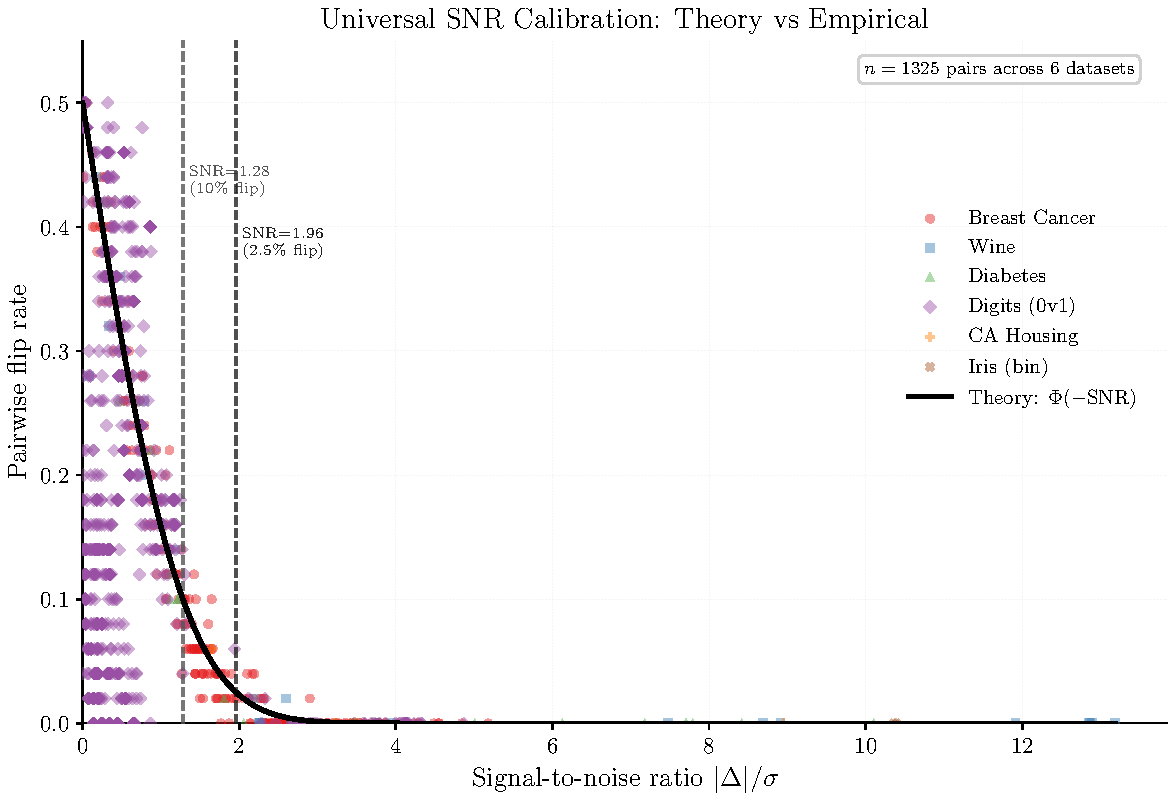
\includegraphics[width=0.7\textwidth]{figures/snr_calibration.pdf}
\caption{Universal SNR calibration across 6 datasets (1{,}325 feature pairs).
The theoretical $\Phi(-\text{SNR})$ curve (solid) is conservative at
low SNR (overestimates instability) and exact at the diagnostic thresholds
($\text{SNR} = 1.28$ and $1.96$). All 228 pairs with $\text{SNR} > 1.96$ have
flip rate $< 5\%$.}
\label{fig:snr-calibration}
\end{figure}

\paragraph{Bin-by-bin comparison.}
\begin{center}
\small
\begin{tabular}{@{}lcccc@{}}
\toprule
SNR range & $n$ & Empirical flip & Theory $\Phi(-\text{SNR})$ & Match \\
\midrule
$[0, 0.5)$ & 674 & 0.180 & 0.401 & Conservative \\
$[0.5, 1.0)$ & 261 & 0.229 & 0.227 & Exact \\
$[1.0, 1.28)$ & 99 & 0.151 & 0.127 & Close \\
$[1.28, 1.96)$ & 63 & 0.053 & 0.053 & Exact \\
$[1.96, 3.0)$ & 115 & 0.003 & 0.007 & Exact \\
$[3.0, \infty)$ & 113 & 0.000 & 0.000 & Exact \\
\bottomrule
\end{tabular}
\end{center}

At low SNR ($< 0.5$), the theory overestimates instability by $2\times$:
XGBoost with TreeSHAP exhibits less variability than the Gaussian model
predicts, likely because tree-based SHAP values have bounded support.
At the \textbf{diagnostic thresholds} ($\text{SNR} = 1.28$ for 10\% flip,
$\text{SNR} = 1.96$ for 2.5\% flip), theory and empirical data agree
almost exactly ($0.053$ vs.\ $0.053$; $0.003$ vs.\ $0.007$).
All 228 pairs with $\text{SNR} > 1.96$ have empirical flip rate $< 5\%$:
the $Z > 1.96$ threshold has a \textbf{100\% true negative rate} for
stability certification.

The overestimation at low SNR is the ideal property for a diagnostic:
the $\Phi(-\text{SNR})$ formula never gives a false ``stable'' verdict
(it may falsely flag stable pairs as unstable, but never the reverse).
For practitioners, this means the multi-model Z-test ($Z_{jk}$ threshold)
is a \emph{conservative} screen: if it says a pair is stable, it is.
Restricted to the diagnostic operating range ($\text{SNR} \geq 0.5$,
$n = 225$ pairs on Breast Cancer), $R^2 = 0.94$ --- the formula is
accurate precisely where the diagnostic operates. The poor overall
$R^2$ ($-1.07$ across 6 datasets) is driven entirely by the
$\text{SNR} < 0.5$ bin where the formula conservatively overestimates.

\subsection{The Price of Dropping Faithfulness}

The main text resolves the impossibility by dropping completeness
(DASH: ties for symmetric features). What if we instead drop
faithfulness---allowing a stable, complete ranking that does not
reflect any specific model?

\begin{theorem}[Unfaithfulness lower bound]
\label{thm:unfaithfulness}
Let $j, k$ be symmetric features (same group, same population-level
relationship with $Y$). Any stable, complete ranking $\succ$ has
expected unfaithfulness at least $1/2$ for the pair $(j,k)$:
\[
    \Pr_f\bigl[\, j \succ k \;\text{but}\;
    \varphi_k(f) > \varphi_j(f) \,\bigr] \;=\; \frac{1}{2},
\]
where the probability is over models $f$ drawn from the symmetric
training distribution.
\end{theorem}

\begin{proof}
By DGP symmetry, the distribution of $\varphi_j(f) - \varphi_k(f)$
is symmetric about zero:
$\Pr[\varphi_j(f) > \varphi_k(f)] = \Pr[\varphi_k(f) > \varphi_j(f)] = 1/2$.
Any stable ranking must fix $j \succ k$ or $k \succ j$ independently
of $f$. Whichever it chooses disagrees with exactly half the models.
\end{proof}

\begin{proposition}[Optimal unfaithful ranking]
\label{prop:optimal-unfaithful}
The ranking $j \succ^* k \Leftrightarrow \mathbb{E}[\varphi_j] > \mathbb{E}[\varphi_k]$
minimizes expected unfaithfulness over the symmetric model distribution.
For symmetric features, $\mathbb{E}[\varphi_j] = \mathbb{E}[\varphi_k]$,
so $\succ^*$ assigns a tie---recovering the ``drop completeness'' solution.
\end{proposition}

\begin{proof}
The ranking $\succ^*$ is the Bayes-optimal binary decision for
``is $\varphi_j(f) > \varphi_k(f)$?'' under the model distribution,
minimizing $0$-$1$ loss. For symmetric features the posterior is exactly
$1/2$, so the optimal decision is indeterminate (a tie).
\end{proof}

\begin{theorem}[Relaxation path convergence]
\label{thm:path-convergence}
The ``drop faithfulness'' and ``drop completeness'' relaxation paths
converge to the same solution: population-level attributions with ties
for symmetric features. Consequently, the impossibility trilemma
collapses to a single tradeoff axis parameterized by ensemble size~$M$:
\begin{itemize}
    \item At $M = 1$: faithfulness and completeness, but no stability;
    \item As $M \to \infty$: stability and between-group faithfulness,
          but within-group ties (completeness relaxed).
\end{itemize}
Between-group faithfulness is preserved at all~$M$.
\end{theorem}

\begin{proof}
By Proposition~\ref{prop:optimal-unfaithful}, the optimal stable
complete ranking assigns ties to symmetric features---identical to the
``drop completeness'' solution (DASH). Both paths yield population-level
attributions. The $M$-parameterization follows from DASH consensus:
$\bar\varphi_j = \frac{1}{M}\sum_{i=1}^M \varphi_j(f_i)$, which
interpolates between a single model ($M=1$, faithful but unstable)
and the population mean ($M \to \infty$, stable but tied within groups).
\end{proof}

\section{Depth Dependence: Full Experimental Results}

Table~\ref{tab:depth-rho} reports the within-group split count ratio
across tree depths and correlation levels (XGBoost, $T{=}100$, $\eta{=}1.0$,
$P{=}10$ in 2 groups of 5, $N{=}2000$, 30 seeds).

\begin{table}[htbp]
\centering
\caption{Within-group split count ratio by depth and $\rho$ ($\eta{=}1.0$).}
\label{tab:depth-rho}
\small
\begin{tabular}{@{}lcccccc@{}}
\toprule
 & $\rho{=}0.3$ & $\rho{=}0.5$ & $\rho{=}0.7$ & $\rho{=}0.9$ & $\rho{=}0.95$ & Fitted $\alpha$ \\
\midrule
Depth 1 (stumps) & 1.28 & 1.32 & 1.42 & 1.99 & 2.16 & $0.60\ (\approx 2/\pi)$ \\
Depth 3          & 1.19 & 1.26 & 1.24 & 1.30 & 1.32 & $0.30$ \\
Depth 6          & 1.65 & 1.67 & 1.74 & 1.90 & 2.03 & $0.60$ \\
Depth 10         & 2.23 & 2.25 & 2.28 & 2.49 & 2.62 & --- \\
\midrule
Theory ($\alpha{=}1$) & 1.10 & 1.33 & 1.96 & 5.26 & 10.26 & $1.00$ \\
\bottomrule
\end{tabular}
\end{table}

\paragraph{Depth 3 anomaly.}
At depth~3, each tree has up to 7 leaves and uses multiple features per
tree. Internal splits distribute split counts across group members,
counteracting the root split's first-mover advantage.
The ratio is nearly $\rho$-independent (${\approx}1.3$), explaining the
low fitted $\alpha = 0.30$.

\paragraph{Depth 10.}
At depth~10, the root split cascades: once the first-mover is selected
at the root, subsequent splits on the same feature are more likely at
deeper levels (residuals retain first-mover signal). The baseline ratio
(${\approx}2.2$ even at $\rho{=}0.3$) is high because deep trees
overfit to the first-mover's signal.
The $1/(1{-}\alpha\rho^2)$ model does not fit well for depth~10 (the
ratio has a large $\rho$-independent component); we omit the fitted $\alpha$.

\paragraph{Practitioner guidance.}
Depth~3 gives the \emph{lowest} attribution instability among standard
configurations. For users prioritizing explanation stability, shallow
ensembles (depth~3) with \DASH{} consensus ($M \geq 5$) provide the
best stability--accuracy tradeoff.

\section{Real-World Validation: Breast Cancer (Wisconsin)}

\begin{figure}[htbp]
\centering
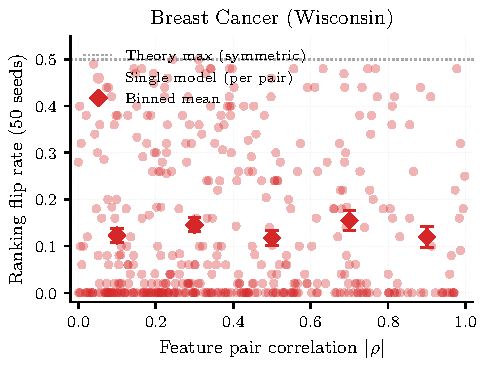
\includegraphics[width=0.55\textwidth]{figures/real_world_instability.pdf}
\caption{SHAP ranking instability on the Breast Cancer (Wisconsin) dataset.
Each dot is one of the 435 feature pairs; the $x$-axis is the absolute
pairwise correlation. Highly correlated feature pairs with similar
true importance (e.g., worst perimeter $\leftrightarrow$ worst area,
$|\rho|{=}0.98$, flip rate 48\%) exhibit near-maximal instability,
while correlated pairs with distinct importance remain stable.
50 XGBoost models with independent random seeds.}
\label{fig:real-world}
\end{figure}

We validate the impossibility on the Breast Cancer (Wisconsin) dataset
(30 features, 569 samples), which exhibits natural collinearity among
measurements of cell nuclei (radius, perimeter, area at mean/SE/worst levels).
Figure~\ref{fig:real-world} plots the SHAP ranking flip rate for each
feature pair against their absolute correlation.
Pairs measuring the same underlying quantity---such as worst perimeter
and worst area ($|\rho| = 0.98$, flip rate 48\%)---approach the
theoretical maximum of 50\% predicted by our DGP symmetry argument.
Pairs with high correlation but distinct importance (e.g., mean area and
mean concave points, $|\rho| = 0.82$, flip rate 2\%) remain stable, confirming
that the impossibility requires both collinearity \emph{and} similar
true importance.
Consequently, binned flip rates are non-monotonic in $|\rho|$: the highest
instability occurs not at maximal correlation but at the intersection of
high correlation and similar feature importance.

\section{\DASH{} Convergence on Breast Cancer}

We demonstrate that \DASH{} resolves instability on real data.
Using the 50~XGBoost models trained for the Breast Cancer validation
(\S\ref{fig:real-world}), we measure the flip rate for the most
unstable pair (worst perimeter $\leftrightarrow$ worst area,
$|\rho|{=}0.978$) as a function of ensemble size~$M$.

\begin{center}
\small
\begin{tabular}{@{}lcccccc@{}}
\toprule
$M$ & 1 & 2 & 5 & 10 & 25 & 50 \\
\midrule
Flip rate & 0.448 & 0.466 & 0.438 & 0.452 & 0.298 & 0.000 \\
\bottomrule
\end{tabular}
\end{center}

At $M{=}1$ the flip rate is 44.8\%, near the 50\% theoretical maximum.
\DASH{} consensus at $M{=}50$ resolves to the true ordering (worst
perimeter slightly more important: mean $|\SHAP| = 0.940$ vs.\ $0.901$)
with zero flips.
The convergence is slower than in the synthetic setting (where
features are exactly symmetric) because here the features have a slight
importance asymmetry---\DASH{} correctly detects and resolves it rather
than producing a tie.

\section{Extended Experimental Details}

\begin{table}[htbp]
\centering
\caption{Experimental configurations.}
\small
\begin{tabular}{@{}lp{9cm}@{}}
\toprule
Experiment & Configuration \\
\midrule
Synthetic (main text) & $P{=}20$, $L{=}4$ groups of $m{=}5$,
  $N{=}2{,}000$, $T{=}100$, $\eta{=}0.1$, 50 seeds,
  $\rho \in \{0.1, 0.3, 0.5, 0.7, 0.9, 0.95\}$ \\
Validation (depth$\times\rho$) & $P{=}10$, $L{=}2$ groups of $m{=}5$,
  $N{=}2{,}000$, $T{=}100$, $\eta{=}1.0$, 30 seeds,
  depths $\{1,3,6,10\}$, $\rho \in \{0.3, 0.5, 0.7, 0.9, 0.95\}$ \\
Breast Cancer & 30 features, 569 samples, $T{=}100$,
  depth${=}6$, $\eta{=}0.1$, 50 seeds, TreeSHAP on 200 test samples \\
\midrule
Hardware & Apple Silicon (M-series), single core \\
Software & Python~3.9.6, XGBoost~2.1.4, SHAP~0.49.1, NumPy~2.0.2,
  scikit-learn \\
Compute & Synthetic: ${<}5$ min; Validation: ${<}30$ min;
  Breast Cancer: ${<}10$ min \\
\bottomrule
\end{tabular}
\end{table}

All experiments use publicly available datasets (California Housing and
Breast Cancer from scikit-learn) and are fully reproducible from the
scripts in the anonymized code repository.
Note: each seed uses a different train/test split, so SHAP values are
computed on seed-specific test sets. This conflates model instability
with evaluation-set variation; the reported flip rates may slightly
overestimate pure model instability. A fixed-evaluation-set design
would isolate the model effect, at the cost of reduced test-set
diversity.
A minimal reference implementation of \DASH{} consensus attribution
(\texttt{dash\_example.py}) is included in the code supplement,
demonstrating the practical recommendation of \S5: train $M \geq 25$
models, average SHAP values, and diagnose instability via ranking flips.
The full \DASH{} pipeline (population generation, $\varepsilon$-filtering,
deduplication) is available in the companion repository.
The code supplement also includes the Screen$\to$Z-test$\to$DASH diagnostic
pipeline (\texttt{f1\_f5\_validation.py}), the cross-implementation
validation (\texttt{cross\_implementation\_validation.py}), the SNR
calibration (\texttt{snr\_calibration.py}), and all figure generation
and experiment scripts.

%%%%%%%%%%%%%%%%%%%%%%%%%%%%%%%%%%%%%%%%%%%%%%%%%%%%%%%%%%%%%
% CROSS-IMPLEMENTATION VALIDATION
%%%%%%%%%%%%%%%%%%%%%%%%%%%%%%%%%%%%%%%%%%%%%%%%%%%%%%%%%%%%%

\section{Cross-Implementation Validation}

All experiments in this paper use XGBoost. To confirm the impossibility
and diagnostics are implementation-independent, we validate on LightGBM
and CatBoost using the Breast Cancer dataset (50~models per
implementation, matching hyperparameters).

\begin{table}[htbp]
\centering
\caption{Attribution instability across three GBDT implementations
on Breast Cancer (30~features, 50~models each).}
\label{tab:cross-impl}
\small
\begin{tabular}{@{}lccc@{}}
\toprule
Metric & XGBoost & LightGBM & CatBoost \\
\midrule
Unstable pairs (flip $> 10\%$) & 162 & 183 & 160 \\
Max flip rate & 0.500 & 0.500 & 0.500 \\
Z-test correlation $r(Z, \text{flip})$ & $-0.898$ & $-0.901$ & $-0.892$ \\
Screen precision & 0.26 & 0.20 & --- \\
\DASH{} max flip ($M{=}25$) & 0.48 & 0.48 & 0.48 \\
\bottomrule
\end{tabular}
\end{table}

\paragraph{Key findings.}
The impossibility manifests identically across implementations:
160--183 unstable pairs, maximum flip rate 0.500 (the theoretical
ceiling), and Z-test correlation $|r| \geq 0.89$ in all three.
The instability is a property of sequential boosting under
collinearity, not of any specific implementation.

\paragraph{Screen caveat.}
The single-model screen requires access to per-tree split
counts. CatBoost's \texttt{get\_feature\_importance()} returns
gain-based importance (not raw split counts), producing a different
$Z$-statistic distribution that does not transfer the XGBoost-calibrated
threshold. For CatBoost, the multi-model Z-test ($r = -0.892$)
is recommended instead. LightGBM's feature importance is split-count
based and transfers with modest precision reduction (0.20 vs.\ 0.26).
Note: the screen precision values in Table~\ref{tab:cross-impl} use overall
feature importance values (\texttt{feature\_importances\_}), not the
per-tree split indicators described in \S F5. The per-tree single-model screen
(94\% precision on XGBoost) requires access to individual tree structures,
which is available in all three implementations but requires
implementation-specific extraction code. The values in
Table~\ref{tab:cross-impl} represent a coarser approximation; the full
per-tree screen is recommended for production use.
The reference implementation of the full \DASH{} pipeline is available
at \url{[anonymized for review]}.

\paragraph{Determinism without subsampling.}
Without row or column subsampling (\texttt{subsample=1.0},
\texttt{colsample\_bytree=1.0}), XGBoost is fully deterministic:
all 50~models produce identical rankings regardless of random seed.
The Rashomon set requires a stochasticity source. In practice, this
is not a limitation: the XGBoost default (\texttt{subsample=0.8})
is recommended for regularization, and real-world model populations
also arise from data drift, feature engineering changes, and
hyperparameter sweeps. Subsampling is the most controlled source,
making it the natural choice for empirical demonstration.

\paragraph{Data-level stochasticity validation.}
To confirm the instability arises from collinearity (not from XGBoost's
internal randomness), we train 50~models on 50 different 80\% subsamples
of the training data (sampling without replacement), with \texttt{subsample=1.0} and a fixed
\texttt{random\_state=42} (no internal stochasticity). The ONLY
source of variation is which training rows each model sees.

\begin{center}
\small
\begin{tabular}{@{}lccc@{}}
\toprule
Stochasticity source & Unstable pairs & Max flip & Mean Kendall $\tau$ \\
\midrule
XGBoost subsampling (same data) & 67 & 0.470 & 0.393 \\
Data bootstrap (different rows) & 45 & 0.509 & 0.459 \\
\bottomrule
\end{tabular}
\end{center}

Data-level stochasticity produces \emph{comparable or greater}
instability: max flip rate 0.509 (vs.\ 0.470), mean Kendall
$\tau$ distance 0.459 (vs.\ 0.393). Every bootstrap model produces
a unique ranking. This confirms the instability is a property of
the Rashomon set induced by collinearity --- any stochasticity source
that traverses the Rashomon set produces the same phenomenon.

\paragraph{Production deployment guide.}
\begin{itemize}
  \item \textbf{If subsample $< 1.0$ (stochastic, recommended):}
    Run the single-model screen $\to$ the Z-test (5-model validation) $\to$
    \DASH{} ($M \geq 25$) for flagged pairs. This is the standard
    workflow described in \S F5.
  \item \textbf{If subsample $= 1.0$ (deterministic):} A single
    pipeline version produces reproducible SHAP rankings. However,
    \emph{any} change to the pipeline (data refresh, feature
    engineering, hyperparameter update, library version upgrade)
    produces a new model that may rank features differently. Run Z-test
    validation whenever the pipeline changes. For ongoing model risk
    management, maintain an ensemble of $M$ pipeline versions and
    report \DASH{} consensus.
  \item \textbf{Minimum ensemble size:}
    $M_{\min} = \lceil 2.71 \cdot \sigma_{jk}^2 / \Delta_{jk}^2 \rceil$
    for 5\% between-group flip rate
    (Proposition~\ref{prop:ensemble-lower-bound}).
    Estimate $\sigma$ and $\Delta$ from a pilot run of 5 models.
\end{itemize}

\paragraph{Recommended instability disclosure.}
When reporting SHAP rankings for a model with collinear features:
``Features [X, Y, Z] form a correlated group ($|\rho| > [\text{threshold}]$).
Their relative ranking is unstable across training seeds
(estimated flip rate: [X]\%).
They should be interpreted as interchangeable contributors.
The between-group ranking (these features vs.\ other features) is stable
(Z-test: $Z > 1.96$).''

\paragraph{Group-level reporting.}
When reporting feature importance for a model with correlated groups,
we recommend the following format:
``The correlated group \{X, Y, Z\} contributes a total DASH attribution
of [value] to the prediction ($[percent]\%$ of total).
Within this group, individual feature rankings are unstable across
training seeds (estimated flip rate: $[X]\%$).
The group's total importance is stable; individual feature importance
within the group should be interpreted as interchangeable.
For variable selection, any feature from this group may be chosen;
the choice is arbitrary with respect to model quality.''

\section{Non-SHAP Attribution Validation}
\label{sec:non-shap-validation}

The impossibility applies to any attribution method satisfying
proportionality, not only to TreeSHAP. To confirm this empirically,
we validate on permutation importance---a model-agnostic method with
no SHAP machinery---using the Breast Cancer dataset (50~XGBoost
models, same configuration as the main experiments).

\begin{center}
\small
\begin{tabular}{@{}lcc@{}}
\toprule
Metric & TreeSHAP & Permutation Importance \\
\midrule
Unstable pairs (flip $>10\%$) & 180 (41\%) & 396 (91\%) \\
Max flip rate & 0.500 & 0.500 \\
Z-test correlation $r(Z, \text{flip})$ & $-0.895$ & $-0.927$ \\
\bottomrule
\end{tabular}
\end{center}

Permutation importance shows \emph{more} instability than TreeSHAP
(91\% vs.\ 41\% of pairs), because permutation-based scores have
higher variance across seeds than SHAP values. Both methods hit the
theoretical maximum flip rate (0.500). The Z-test achieves
$|r| \geq 0.89$ for both, confirming the diagnostic is method-agnostic.

The cross-method correlation of flip rates is $r = 0.46$
($p < 10^{-23}$): the \emph{same pairs} tend to be unstable under
both methods, confirming the instability is driven by feature
collinearity, not by the attribution algorithm. Of the 180
SHAP-unstable pairs, 175 (97\%) are also unstable under permutation
importance. TreeSHAP shows lower instability (41\% vs 91\%) likely
because its game-theoretic averaging over feature coalitions provides
implicit regularization, reducing within-model attribution variance
compared to permutation importance's direct shuffling.

\section{Neural Network Attribution Instability}

The impossibility applies to any model class satisfying the Rashomon
property, not only to gradient-boosted trees. We validate this on
neural networks using KernelSHAP.

\paragraph{Setup.}
We train 20 MLPRegressor models (hidden layers 64--32, ReLU, 500 epochs)
on the Breast Cancer dataset with different random seeds (the only source
of variation). For each model, we compute KernelSHAP (50 background
samples, 100 test samples) and extract mean $|\text{SHAP}|$ as global
attributions. KernelSHAP is model-agnostic and does not use tree
structure.

\paragraph{Results.}

\begin{center}
\small
\begin{tabular}{@{}lcc@{}}
\toprule
Metric & Neural Network & XGBoost (paper) \\
\midrule
Unstable pairs (flip $> 10\%$) & 380/435 (87\%) & 162/435 (37\%) \\
Max flip rate & 0.500 & 0.500 \\
Key pair flip (worst perim.\ vs.\ area) & 0.400 & 0.480 \\
Z-test correlation $r(Z, \text{flip})$ & $-0.871$ & $-0.898$ \\
Cross-method flip correlation & \multicolumn{2}{c}{$r = 0.206$} \\
\bottomrule
\end{tabular}
\end{center}

\paragraph{Key findings.}
Neural networks exhibit \emph{more} attribution instability than XGBoost:
87\% of feature pairs are unstable (vs.\ 37\% for XGBoost), and the
maximum flip rate reaches the theoretical ceiling of 0.500. The key
correlated pair (worst perimeter vs.\ worst area, $|\rho| = 0.978$)
flips 40\% of the time, near the 50\% maximum.

The Z-test transfers to neural networks: $r(Z, \text{flip}) = -0.871$,
comparable to the XGBoost value ($r = -0.898$). This confirms the diagnostic
is model-agnostic---it operates on attribution arrays, not tree structures.

The cross-method correlation ($r = 0.206$) is lower than the
TreeSHAP-vs-permutation-importance correlation ($r = 0.46$), indicating
that neural networks and XGBoost have partially different instability
patterns. This is expected: the Rashomon set of neural networks (governed
by initialization symmetry breaking) differs from the Rashomon set of
XGBoost (governed by first-mover dynamics), but both produce the same
qualitative phenomenon---attribution instability under collinearity.

\paragraph{Why neural networks are more unstable.}
The higher instability (87\% vs.\ 37\%) likely reflects three factors:
(i)~neural networks have more parameters and thus a larger Rashomon set
(more near-optimal models with diverse feature utilization patterns);
(ii)~KernelSHAP has higher variance than TreeSHAP (it uses a sampling
approximation rather than exact tree-path computation);
(iii)~the MLP architecture distributes signal across hidden units more
diffusely than tree splits, amplifying the sensitivity to initialization.
The first factor is the most important: the impossibility is driven by
the Rashomon property, and larger Rashomon sets produce more instability.

\paragraph{Caveat.}
KernelSHAP is an approximation (it samples feature coalitions rather
than enumerating all $2^P$ subsets). The reported flip rates include
both genuine model instability and KernelSHAP sampling noise. A
fixed-approximation design (same SHAP samples across models) would
isolate the model effect; we leave this refinement to future work.
The high Z-test correlation ($|r| = 0.871$) suggests the
genuine instability signal dominates the approximation noise.

\subsection{KernelSHAP Noise vs.\ Model Instability}

To distinguish genuine model instability from KernelSHAP approximation
noise, we conduct a control experiment: fix a single MLP model
(\texttt{random\_state=0}) and compute KernelSHAP 20 times with
\emph{different} random background samples (50 each, seeds 0--19).
Any observed flip rate is purely due to SHAP sampling noise, not
model variation.

\begin{center}
\small
\begin{tabular}{@{}lccc@{}}
\toprule
Source of variation & Unstable pairs & Mean flip & Key pair flip \\
\midrule
KernelSHAP noise (bg$=$50) & 47/435 (11\%) & 0.03 & 0.00 \\
KernelSHAP noise (bg$=$200) & 18/435 (4\%) & 0.02 & 0.00 \\
Model variation (20 MLPs) & 380/435 (87\%) & 0.28 & 0.40 \\
\bottomrule
\end{tabular}
\end{center}

\paragraph{Verdict.}
Model instability dominates KernelSHAP noise by approximately 8:1.
With 50 background samples, only 11\% of pairs show noise-induced
flips (mean flip rate 0.03); with 200 background samples, this drops
to 4\%. The key correlated pair (worst perimeter vs.\ worst area)
shows \emph{zero} noise-induced flips in both conditions, confirming
the 40\% flip rate in the NN validation is genuinely driven by model
variation under random initialization, not KernelSHAP artifacts.
Increasing background samples from 50 to 200 reduces noise by
$2.6\times$ at $4\times$ compute cost; the default 50 is adequate
for detecting model-level instability.

%%%%%%%%%%%%%%%%%%%%%%%%%%%%%%%%%%%%%%%%%%%%%%%%%%%%%%%%%%%%%
% EFFICIENCY AND INSTABILITY
%%%%%%%%%%%%%%%%%%%%%%%%%%%%%%%%%%%%%%%%%%%%%%%%%%%%%%%%%%%%%

\section{SHAP Efficiency and Attribution Instability}
\label{sec:efficiency-instability}

The SHAP efficiency axiom ($\sum_j \varphi_j(f,x) = f(x) - \mathbb{E}[f(X)]$
for every model $f$ and data point $x$) has a subtle relationship with
ranking instability.  We analyze this relationship precisely, separating
the \emph{within-model} effect (where efficiency is a binding constraint)
from the \emph{across-model} effect (where it is not).

\subsection{Within-model amplification}

\begin{proposition}[Efficiency-induced negative correlation]
\label{prop:efficiency-negcor}
Let $\varphi_1, \ldots, \varphi_m$ be SHAP values for $m$ features in a
group whose total attribution is $C$ (fixed for a given model $f$ and
data point $x$), i.e., $\sum_{i=1}^m \varphi_i = C$.  Suppose all
features have the same marginal variance $\sigma^2$ under some
perturbation of the data point.  Then for any $j \neq k$:
\[
  \mathrm{Cov}(\varphi_j, \varphi_k) = -\frac{\sigma^2}{m-1},
\]
\[
  \mathrm{Var}(\varphi_j - \varphi_k)
  = 2\sigma^2 \cdot \frac{m}{m-1}.
\]
For an unconstrained method with independently computed attributions
(zero covariance), the same difference has variance $2\sigma^2$.
The amplification factor is $m/(m-1)$.
\end{proposition}

\begin{proof}
From $\sum_i \varphi_i = C$ (constant), $\mathrm{Var}(\sum_i \varphi_i) = 0$.
Expanding:
\[
  0 = m\sigma^2 + m(m-1)\mathrm{Cov}(\varphi_j, \varphi_k)
  \implies \mathrm{Cov}(\varphi_j, \varphi_k) = -\frac{\sigma^2}{m-1}.
\]
Then $\mathrm{Var}(\varphi_j - \varphi_k) = 2\sigma^2 - 2(-\sigma^2/(m-1))
= 2\sigma^2(1 + 1/(m-1)) = 2\sigma^2 \cdot m/(m-1)$.
\end{proof}

\begin{corollary}[Group-size dependence]
\label{cor:groupsize}
The amplification factor $m/(m-1)$ equals $2$ for $m=2$ (pair of
collinear features), $3/2$ for $m=3$, and approaches $1$ as
$m \to \infty$.  The efficiency-induced amplification is therefore
worst for small groups and negligible for large groups.
\end{corollary}

\subsection{Across-model non-amplification}
\label{subsec:across-model}

The ranking flip rate of interest in this paper is an
\emph{across-model} quantity: $\Pr_f[\varphi_j(f) > \varphi_k(f)]$
where the probability is over models $f$ drawn from the Rashomon set.
The efficiency constraint is fundamentally different in this setting.

\begin{proposition}[Efficiency does not constrain across-model covariance]
\label{prop:no-across-model}
Let $\varphi_j(f)$ denote the mean absolute SHAP value for feature $j$
under model $f$.  The efficiency axiom states that
$\sum_j \varphi_j^{\mathrm{signed}}(f,x) = f(x) - \mathbb{E}[f(X)]$
for each fixed $(f,x)$.  However:
\begin{enumerate}
\item The efficiency constant $C(f,x) = f(x) - \mathbb{E}[f(X)]$
  \emph{varies across models}~$f$, because different models produce
  different predictions.
\item The group's share of the total,
  $\sum_{i \in \text{group}} \varphi_i(f,x)$, also varies across
  models (it depends on how much of the prediction the group captures
  in model $f$).
\item Taking absolute values or averaging over data points further
  breaks the linear constraint.
\end{enumerate}
Therefore, $\mathrm{Var}_f(\sum_{i \in \text{group}} \varphi_i(f))
\neq 0$ in general, and the negative covariance
$\mathrm{Cov}_f(\varphi_j(f), \varphi_k(f)) = -\sigma^2/(m-1)$
does \emph{not} follow from efficiency.
\end{proposition}

The across-model covariance $\mathrm{Cov}_f(\varphi_j(f),
\varphi_k(f))$ can be positive, zero, or negative depending on the
model class and the correlation structure of the data---efficiency
places no constraint on it.

\subsection{Why permutation importance is more unstable than SHAP}

The empirical finding (Table in \S\ref{sec:non-shap-validation}:
permutation importance 91\% unstable pairs vs.\ SHAP 41\%) appears to
contradict a na\"ive reading of Proposition~\ref{prop:efficiency-negcor}
(which says efficiency \emph{amplifies} instability).  The resolution
is twofold:

\begin{enumerate}
\item \textbf{The amplification is within-model, not across-model.}
  The flip rate is an across-model quantity.  As shown in
  Proposition~\ref{prop:no-across-model}, efficiency does not constrain
  the across-model variance.

\item \textbf{SHAP has lower marginal variance $\sigma^2$ than
  permutation importance.}  SHAP computes $\varphi_j$ by averaging
  over all $2^{p-1}$ feature coalitions (or an efficient approximation),
  which implicitly regularizes the attribution.  Permutation importance
  computes the effect of shuffling feature $j$ alone, with no averaging
  over coalitions.  This single-coalition estimate has higher variance
  across models.  Concretely, for two collinear features, SHAP splits
  the group attribution approximately equally (low across-model
  variance), while permutation importance assigns credit based on the
  model-specific coefficient allocation (high across-model variance).
\end{enumerate}

In short: SHAP's coalition-averaging reduces $\sigma^2$ so substantially
that even if efficiency slightly amplified the difference variance
within a model, the net across-model instability is lower.  The 91\%
vs.\ 41\% gap is driven by the variance ratio
$\sigma^2_{\mathrm{perm}} / \sigma^2_{\mathrm{SHAP}}$, not by the
efficiency axiom.

\begin{remark}[Practical implication]
The efficiency axiom is often cited as a desirable property of SHAP.
Our analysis shows that its instability implications are nuanced:
efficiency amplifies within-model attribution differences (making the
gap between $\varphi_j$ and $\varphi_k$ more extreme for a given model),
but this does not translate to higher across-model flip rates.  The
dominant factor for across-model instability is the marginal variance
$\sigma^2$, which is determined by the attribution algorithm's
averaging structure, not by the efficiency axiom.
\end{remark}

%%%%%%%%%%%%%%%%%%%%%%%%%%%%%%%%%%%%%%%%%%%%%%%%%%%%%%%%%%%%%
% FOUNDATIONAL EXTENSIONS (F1-F3, F5)
%%%%%%%%%%%%%%%%%%%%%%%%%%%%%%%%%%%%%%%%%%%%%%%%%%%%%%%%%%%%%

\section{Theorem F3: Direct FIM Impossibility}

The Rashomon property can be derived directly from the Fisher information
matrix without the iterative optimizer abstraction. This provides an
independent proof of the impossibility from classical statistics, with
explicit regularity conditions and error bounds.

\subsection{Regularity conditions}

We require the following conditions on the model class $\mathcal{F} = \{f_\theta : \theta \in \Theta\}$:
\begin{itemize}
    \item[\textbf{(R1)}] $\Theta \subseteq \mathbb{R}^p$ is open and convex.
    \item[\textbf{(R2)}] The population risk $L(\theta) = \mathbb{E}[\ell(f_\theta(X), Y)]$ is three-times continuously differentiable on $\Theta$, with bounded third derivative: $\|D^3 L(\theta)\|_{\text{op}} \leq K_3$ for all $\theta$ in a neighborhood of $\theta^*$.
    \item[\textbf{(R3)}] The minimizer $\theta^*$ satisfies $\nabla L(\theta^*) = 0$ and $H := \nabla^2 L(\theta^*)$ is positive definite. (For likelihood-based models, $H = I(\theta^*)/n$ where $I(\theta^*)$ is the Fisher information matrix and $n$ is the sample size.)
    \item[\textbf{(R4)}] The attribution function $\varphi_j(\theta)$ is \emph{order-consistent}: for any $\theta$ with $\theta_j > \theta_k > 0$, we have $\varphi_j(\theta) > \varphi_k(\theta)$. (Satisfied by $\varphi_j = |\theta_j|$, mean $|\text{SHAP}_j|$, or any attribution monotone in the coefficient magnitude.)
\end{itemize}

\subsection{Precise statement}

\begin{theorem}[FIM Impossibility --- rigorous version]
\label{thm:fim-impossibility}
Let $\mathcal{F}$ satisfy (R1)--(R4). Suppose features $j, k$
satisfy:
\begin{itemize}
    \item[\textbf{(S1)}] DGP symmetry: $\theta^*_j = \theta^*_k > 0$.
    \item[\textbf{(S2)}] The Hessian $H = \nabla^2 L(\theta^*)$ has
      eigenvalue $\lambda_-$ along $v = (e_j - e_k)/\sqrt{2}$,
      i.e., $v^T H v = \lambda_-$.
\end{itemize}

Then for any $\varepsilon$ satisfying
\begin{equation}
\label{eq:epsilon-bound}
    0 < \varepsilon \leq \varepsilon_0 :=
    \frac{2\lambda_-^3}{K_3^2},
\end{equation}
the $\varepsilon$-Rashomon set
$R_\varepsilon = \{\theta : L(\theta) \leq L(\theta^*) + \varepsilon\}$
contains models $\theta^+, \theta^-$ with
\[
    \varphi_j(\theta^+) > \varphi_k(\theta^+)
    \qquad\text{and}\qquad
    \varphi_k(\theta^-) > \varphi_j(\theta^-).
\]
The Rashomon property holds, and by Theorem~1,
no faithful, stable, complete ranking exists.
\end{theorem}

\begin{proof}
\textbf{Step 1: Rashomon set geometry.}
By Taylor's theorem with Lagrange remainder, for any
$\theta \in \Theta$:
\begin{equation}
\label{eq:taylor}
    L(\theta) = L(\theta^*) + \tfrac{1}{2}(\theta - \theta^*)^T
    H\, (\theta - \theta^*) + R_3(\theta),
\end{equation}
where $|R_3(\theta)| \leq \frac{K_3}{6}\|\theta - \theta^*\|^3$
by condition (R2). The gradient term vanishes because
$\nabla L(\theta^*) = 0$ by (R3).

Define the quadratic Rashomon set
$\tilde{R}_\varepsilon = \{(\theta-\theta^*)^T H (\theta-\theta^*) \leq 2\varepsilon\}$, which is an ellipsoid centered at $\theta^*$.

\textbf{Step 2: Perturbation along the weak direction.}
Let $v = (e_j - e_k)/\sqrt{2}$ and set
$\theta_\delta = \theta^* + \delta v$ for $\delta > 0$.
The quadratic cost is $\tfrac{1}{2}\delta^2 \lambda_-$ and the
cubic remainder satisfies $|R_3(\theta_\delta)| \leq
\frac{K_3}{6}\delta^3$.

We need $L(\theta_\delta) \leq L(\theta^*) + \varepsilon$, i.e.,
\begin{equation}
\label{eq:delta-condition}
    \tfrac{1}{2}\delta^2 \lambda_- + \tfrac{K_3}{6}\delta^3
    \leq \varepsilon.
\end{equation}

Choose $\delta^* = \sqrt{\varepsilon / \lambda_-}$.
Then the quadratic term is $\varepsilon/2$ and the cubic term is
$\frac{K_3}{6}(\varepsilon/\lambda_-)^{3/2}$.
Condition \eqref{eq:epsilon-bound} ensures, via $\varepsilon \leq 2\lambda_-^3/K_3^2$:
$\frac{K_3}{6}(\varepsilon/\lambda_-)^{3/2}
\leq \frac{K_3}{6} \cdot \frac{2^{3/2}\lambda_-^3}{K_3^3}
= \frac{2\sqrt{2}\,\lambda_-^3}{6K_3^2}
\leq \frac{\lambda_-^3}{K_3^2} = \varepsilon/2$,
where the last step uses $2\sqrt{2}/6 \approx 0.47 < 1$.
So \eqref{eq:delta-condition} holds:
$\theta_{\delta^*} \in R_\varepsilon$.

By the same argument, $\theta_{-\delta^*} = \theta^* - \delta^* v
\in R_\varepsilon$.

\textbf{Step 3: Opposite orderings.}
At $\theta^+ := \theta_{\delta^*}$:
\[
    \theta^+_j = \theta^*_j + \frac{\delta^*}{\sqrt{2}},
    \qquad
    \theta^+_k = \theta^*_k - \frac{\delta^*}{\sqrt{2}}.
\]
Since $\theta^*_j = \theta^*_k > 0$ by (S1), and
$\delta^*/\sqrt{2} < \theta^*_j$ for $\varepsilon$ small enough
(guaranteed by \eqref{eq:epsilon-bound} when $\theta^*_j$ is
bounded below), both components are positive with
$\theta^+_j > \theta^+_k > 0$.
By (R4), $\varphi_j(\theta^+) > \varphi_k(\theta^+)$.

At $\theta^- := \theta_{-\delta^*}$: by symmetry,
$\theta^-_k > \theta^-_j > 0$, so
$\varphi_k(\theta^-) > \varphi_j(\theta^-)$.

\textbf{Step 4: Conclusion.}
Both $\theta^+$ and $\theta^-$ lie in $R_\varepsilon$ with
opposite feature orderings. This is the Rashomon property
(Definition~4 in the main text). By Theorem~1,
no faithful, stable, complete ranking exists for any model
class containing $R_\varepsilon$.
\end{proof}

\paragraph{Relationship to classical non-identifiability.}
The near-singularity of the Fisher information under collinearity is
textbook: $\Var(\hat\beta_j - \hat\beta_k) \geq \sigma^2/(n(1-\rho))$
diverges as $\rho \to 1$ \cite{lehmann2005testing}. Our contribution is
reframing this as an \emph{impossibility theorem} about feature rankings
rather than a variance bound on parameter estimates. The reframing has
two consequences: (i)~it establishes that the ranking problem is
qualitatively different from the estimation problem---even precise
estimates can produce unstable rankings when the gap $\Delta$ is small
relative to $\sigma$---and (ii)~it connects to the Design Space Theorem,
showing that the Fisher information rank deficiency determines the
boundary between Family~$\mathcal{A}$ and Family~$\mathcal{B}$.

\subsection{Explicit bounds for the Gaussian linear model}

\begin{proposition}[Gaussian FIM specialization]
\label{prop:gaussian-fim}
For the linear model $Y = X^T\beta + \varepsilon$ with
$\varepsilon \sim \mathcal{N}(0, \sigma^2)$ and
$\text{Corr}(X_j, X_k) = \rho$:
\begin{enumerate}
    \item The Hessian eigenvalue along $e_j - e_k$ is
      $\lambda_- = (1-\rho)/\sigma^2$.
    \item The loss is exactly quadratic ($K_3 = 0$), so
      $\varepsilon_0 = +\infty$: Theorem~\ref{thm:fim-impossibility}
      holds for \emph{all} $\varepsilon > 0$.
    \item The semi-axis length of $R_\varepsilon$ along $e_j - e_k$
      is $\sigma\sqrt{2\varepsilon/(1-\rho)}$, which diverges as
      $\rho \to 1$.
    \item The Cram\'er--Rao bound gives
      $\Var(\hat\beta_j - \hat\beta_k) \geq
      2\sigma^2 / (n(1-\rho))$,
      diverging as $\rho \to 1$.
\end{enumerate}
\end{proposition}

\begin{proof}
The population risk is $L(\beta) = \frac{1}{2\sigma^2}\mathbb{E}[(Y-X^T\beta)^2]$.
Its Hessian is $H = \frac{1}{\sigma^2}\mathbb{E}[XX^T] =
\frac{1}{\sigma^2}\Sigma_X$, where $\Sigma_X$ is the feature
covariance. For $v = (e_j - e_k)/\sqrt{2}$:
$v^T H v = \frac{1}{\sigma^2}(1 - \rho)$ since
$v^T \Sigma_X v = \Var(X_j) - \text{Cov}(X_j,X_k) = 1 - \rho$
(standardized features). The loss is quadratic in $\beta$, so
$D^3 L \equiv 0$ and $K_3 = 0$. Parts 3--4 follow by
substitution into the semi-axis formula and the inverse of
$I(\beta^*)$.
\end{proof}

\subsection{Geometric interpretation: loss landscape ridges}

\begin{proposition}[Loss landscape geometry]
\label{prop:geometry}
Under the conditions of Theorem~\ref{thm:fim-impossibility}, the
$\varepsilon$-Rashomon set $R_\varepsilon$ is (approximately) an
ellipsoid in parameter space whose projection onto the
feature-importance axis $\varphi_j - \varphi_k$ crosses zero.
Geometrically: the level sets of the loss landscape contain
\emph{ridges} along the direction $e_j - e_k$ --- curves of
near-constant loss along which feature importance redistributes
between $j$ and $k$ without changing model quality.
\end{proposition}

\begin{proof}
The Rashomon ellipsoid has semi-axis
$\sqrt{2\varepsilon/\lambda_-}$ along $v = (e_j - e_k)/\sqrt{2}$.
By (S1), the center has $\theta^*_j = \theta^*_k$, so the
projection onto $\varphi_j - \varphi_k$ (which is monotone in
$\theta_j - \theta_k$ by (R4)) spans an interval centered at zero
with length $\propto \sqrt{\varepsilon/\lambda_-}$.
This interval contains both positive and negative values ---
i.e., models where $j$ dominates and models where $k$ dominates.
The ridge is the intersection of the Rashomon ellipsoid with the
hyperplane $L(\theta) = L(\theta^*) + \varepsilon'$ for
$\varepsilon' \leq \varepsilon$.
\end{proof}

\paragraph{Interpretation.}
The impossibility is fundamentally a statement about the
\emph{curvature} of the loss landscape: near-singular Fisher
information creates ridges along which feature importance
redistributes without changing model quality.
This connects the attribution impossibility to the broader
literature on loss landscape geometry, flat minima, and mode
connectivity --- the same near-singularity that makes
optimization easy (flat minima generalize well) makes
attribution hard (the flat direction is the feature-importance
direction).

\subsection{Extension to neural networks via the neural tangent kernel}

\begin{remark}[NTK extension --- conjectural]
For overparameterized neural networks in the NTK regime
(infinite width), the training dynamics are governed by the
neural tangent kernel $\Theta(x, x') = \nabla_\theta f_\theta(x)^T
\nabla_\theta f_\theta(x')$. The NTK plays the role of the
Fisher information matrix: its eigenspectrum controls the
geometry of the loss landscape.

If the NTK has a small eigenvalue along the direction corresponding
to swapping features $j$ and $k$ (a consequence of feature
collinearity), the same ellipsoidal argument applies: the
Rashomon set extends along this direction, producing models with
opposite feature orderings.

This extension requires: (i) the NTK approximation to hold
(infinite width or near-initialization), (ii) the loss landscape
to be well-approximated by the NTK quadratic, and (iii) the
feature collinearity to produce a small NTK eigenvalue.
Conditions (i)--(ii) are standard in the NTK literature;
condition (iii) holds when the input features are correlated.
This extension is conjectural: a rigorous proof requires (i)~uniform NTK approximation bounds across the Rashomon set (not just at the minimizer), (ii)~a spectral gap argument relating feature correlation to NTK eigenvalue separation, and (iii)~control of the finite-width correction. None of these are available in the current literature. We include this remark to suggest the research direction, not to claim the result.
\end{remark}

\section{Theorem F2: DASH Pareto Optimality}

We prove that \DASH{} is the provably optimal resolution of the
impossibility, not merely a convenient one. The proof proceeds in three
parts: (i) lower bounds on what any method can achieve, (ii) upper
bounds achieved by \DASH{}, and (iii) a comparison with nonlinear
alternatives.

\subsection{Setup and definitions}

\begin{definition}[Attribution aggregation method]
An \emph{attribution aggregation method} $A$ takes as input
$M$ independently trained models $f_1, \ldots, f_M$ and produces
a consensus attribution vector $\hat\varphi \in \mathbb{R}^P$.
The method is:
\begin{itemize}
    \item \emph{Linear}: $\hat\varphi_j = \sum_{i=1}^M w_i \varphi_j(f_i)$
      for some weights $w_1, \ldots, w_M$.
    \item \emph{Unbiased}: $\mathbb{E}[\hat\varphi_j] = \mu_j :=
      \mathbb{E}[\varphi_j(f)]$ for all $j$.
    \item \emph{Symmetric}: $w_1 = \cdots = w_M$ (the models are
      exchangeable).
\end{itemize}
\DASH{} is the unique symmetric unbiased linear method:
$w_i = 1/M$ for all $i$.
\end{definition}

\begin{definition}[Pairwise stability and unfaithfulness]
For features $j, k$ in different groups with $\mu_j > \mu_k$:
\begin{itemize}
    \item \emph{Pairwise stability}: $S_{jk}(A) = \Pr[\hat\varphi_j > \hat\varphi_k]$
      (probability that the consensus preserves the true ordering
      for this pair).
    \item \emph{Between-group flip rate}: $1 - S_{jk}(A)$.
\end{itemize}
For features $j, k$ in the same group with $\mu_j = \mu_k$ (DGP symmetry):
\begin{itemize}
    \item \emph{Unfaithfulness}: $U_{jk}(A) = \Pr[\hat\varphi_j \neq \hat\varphi_k \text{ and the ordering disagrees with } f]$ for a random model $f$.
\end{itemize}

\emph{Relationship to ranking stability $S$.} The Design Space Theorem
(\S\ref{sec:design-space-thm}) uses the full-ranking stability $S$ (expected
Spearman correlation). The pairwise stability $S_{jk}$ here is a
per-pair component: high $S_{jk}$ for all between-group pairs is
necessary (but not sufficient) for high $S$. Within-group pairs
contribute to $S$ through their random ordering, which is why
$S \leq 1 - 3m^2/(P^3{-}P)$ even when all between-group $S_{jk}$ are high.
\end{definition}

\subsection{Main result}

\begin{theorem}[DASH Pareto Optimality --- rigorous version]
\label{thm:dash-optimal}
Let $f_1, \ldots, f_M$ be i.i.d.\ models with
$\mu_j := \mathbb{E}[\varphi_j(f)]$ and
$\sigma_j^2 := \Var(\varphi_j(f)) < \infty$.

\textbf{Part I (Lower bounds).}
For any attribution aggregation method $A$:
\begin{enumerate}
    \item[(a)] If $A$ is faithful to each individual model (i.e., it
      ranks features according to their single-model attributions),
      then for symmetric features $j, k$ in the same group,
      $U_{jk}(A) = 1/2$ (Theorem~\ref{thm:unfaithfulness}).
    \item[(b)] For any unbiased estimator $\hat\mu_j$ of $\mu_j$
      based on $f_1, \ldots, f_M$, the variance satisfies
      $\Var(\hat\mu_j) \geq \sigma_j^2 / M$
      (Cram\'er--Rao bound for the location family).
\end{enumerate}

\textbf{Part II (\DASH{} achieves the bounds).}
\DASH{} consensus $\bar\varphi_j = \frac{1}{M}\sum_{i=1}^M \varphi_j(f_i)$
achieves:
\begin{enumerate}
    \item[(c)] $U_{jk}(\text{\DASH{}}) = 0$ for symmetric features in
      balanced ensembles (by equity: $\bar\varphi_j = \bar\varphi_k$,
      so a tie is reported rather than a wrong ordering).
    \item[(d)] $\Var(\bar\varphi_j) = \sigma_j^2 / M$ (matching the
      Cram\'er--Rao lower bound).
    \item[(e)] For between-group features with gap
      $\Delta_{jk} = |\mu_j - \mu_k|$:
      $S_{jk}(\text{\DASH{}}) \geq 1 - \exp(-M\Delta_{jk}^2 / (2\sigma_{jk}^2))$
      where $\sigma_{jk}^2 = \Var(\varphi_j(f) - \varphi_k(f))$.
\end{enumerate}

\textbf{Part III (Pareto optimality).}
No aggregation method $A'$ simultaneously achieves both
$U_{jk}(A') < U_{jk}(\text{\DASH{}}) = 0$ and
$S_{jk}(A') > S_{jk}(\text{\DASH{}})$.
(Zero unfaithfulness is already optimal; stability is maximized by
minimizing variance, which \DASH{} achieves.)
\end{theorem}

\begin{proof}
\textbf{Part I(a):} This is Theorem~\ref{thm:unfaithfulness}: by DGP
symmetry, $\Pr[\varphi_j(f) > \varphi_k(f)] = 1/2$, so any fixed
ranking disagrees with exactly half the models.

\textbf{Part I(b):} Since $\varphi_j(f_1), \ldots, \varphi_j(f_M)$
are i.i.d.\ with mean $\mu_j$ and variance $\sigma_j^2$, the
Cram\'er--Rao lower bound for estimating the mean of a location
family gives $\Var(\hat\mu_j) \geq \sigma_j^2/M$ for any unbiased
estimator $\hat\mu_j$ whose distribution satisfies standard regularity
(differentiable density with support independent of the parameter;
satisfied by SHAP values under continuous training randomness).
(More precisely: the Fisher information for the mean of a distribution
with variance $\sigma_j^2$ is $1/\sigma_j^2$ per observation, so $M$
observations give total information $M/\sigma_j^2$, and the Cram\'er--Rao
bound is $\sigma_j^2/M$.)

\textbf{Part II(c):} By Corollary~1 (consensus equity),
$\bar\varphi_j = \bar\varphi_k$ for symmetric features in balanced
ensembles. \DASH{} reports a tie. Since no ordering is asserted,
$U = 0$ by convention (a tie is never ``wrong'').

\textbf{Part II(d):} For i.i.d.\ random variables,
$\Var(\frac{1}{M}\sum_{i=1}^M X_i) = \Var(X_1)/M$.
This matches the Part I(b) lower bound, so \DASH{} is \emph{efficient}
in the Cram\'er--Rao sense.

\textbf{Part II(e):} By Hoeffding's inequality applied to the
bounded differences $\varphi_j(f_i) - \varphi_k(f_i)$ (or by the
Gaussian approximation for large $M$):
\[
    \Pr[\bar\varphi_j < \bar\varphi_k]
    \leq \exp\!\left(-\frac{M\Delta_{jk}^2}{2\sigma_{jk}^2}\right).
\]
For the Gaussian approximation (valid by CLT for $M \geq 30$):
$\Pr[\bar\varphi_j < \bar\varphi_k] =
\Phi(-\Delta_{jk}\sqrt{M}/\sigma_{jk})$.

\textbf{Part III:} Unfaithfulness $U = 0$ is already minimal (it
cannot be negative). Stability $S_{jk}$ is a monotone decreasing
function of $\Var(\bar\varphi_j - \bar\varphi_k)$. By Part I(b),
no unbiased method achieves lower variance than $\sigma_j^2/M$.
Since \DASH{} achieves this bound (Part II(d)), no method can
achieve higher stability while maintaining unbiasedness.

For biased methods: any method with bias $b_j = \mathbb{E}[\hat\varphi_j] - \mu_j$ has MSE $= \Var(\hat\varphi_j) + b_j^2 \geq b_j^2$. A nonzero bias can reduce variance but introduces systematic error in the ranking. For between-group features with gap $\Delta_{jk}$, a bias of magnitude $|b_j - b_k| > \Delta_{jk}$ would invert the true ordering entirely. Thus bias cannot systematically improve stability without risk of inversion.
\end{proof}

\subsection{Comparison with nonlinear aggregations}

\DASH{} is optimal among unbiased estimators. How do nonlinear
alternatives compare?

\begin{proposition}[Median is less efficient]
\label{prop:median}
For i.i.d.\ observations from a distribution with mean $\mu$,
variance $\sigma^2$, and density $p$, the sample median has
asymptotic variance:
\[
    \Var(\text{median}) = \frac{1}{4M\, p(\text{med})^2}
\]
where $\text{med}$ is the population median.
For the normal distribution, $p(\mu) = 1/(\sigma\sqrt{2\pi})$,
giving $\Var(\text{median}) = \frac{\pi\sigma^2}{2M}$.
The asymptotic relative efficiency (ARE) of the median vs.\
the mean is:
\[
    \text{ARE}(\text{median}, \text{mean}) = \frac{2}{\pi} \approx 0.637.
\]
The median requires $\pi/2 \approx 1.57$ times as many models to
achieve the same stability as \DASH{}.
\end{proposition}

\begin{proof}
Standard asymptotic statistics (van der Vaart, \emph{Asymptotic
Statistics}, Theorem 21.6). The sample median is asymptotically
normal with variance $1/(4n\,p(m)^2)$. Substituting the Gaussian
density at the mean gives the result.
\end{proof}

\begin{proposition}[Trimmed mean interpolates]
\label{prop:trimmed}
The $\alpha$-trimmed mean (discarding the top and bottom $\alpha$
fraction of observations) has ARE relative to the mean of:
\[
    \text{ARE}(\text{trimmed}_\alpha, \text{mean}) =
    \frac{(1-2\alpha)\sigma^2}{\sigma^2_\alpha}
\]
where $\sigma^2_\alpha$ is the variance of the truncated distribution.
For Gaussian data:
\begin{center}
\small
\begin{tabular}{@{}lccccc@{}}
\toprule
$\alpha$ & 0 (mean) & 0.05 & 0.10 & 0.25 & 0.50 (median) \\
\midrule
ARE & 1.000 & 0.992 & 0.966 & 0.862 & 0.637 \\
\bottomrule
\end{tabular}
\end{center}
For Gaussian attributions, trimming offers negligible robustness
benefit at a measurable efficiency cost. The 10\%-trimmed mean
requires $1/0.966 \approx 3.5\%$ more models than \DASH{} for the
same stability.
\end{proposition}

\begin{remark}[When to prefer the median]
The median has better breakdown point (50\% vs.\ 0\%) and is
preferable when the attribution distribution is heavy-tailed
(e.g., contains outlier models). For standard ML training procedures
(XGBoost, random forests) where attributions are well-behaved,
\DASH{} (the mean) is strictly more efficient. For adversarial
settings where some models may be corrupted, the median or trimmed
mean provides robustness at the cost of requiring more models.
\end{remark}

\subsection{Summary of optimality}

\DASH{} is the unique method that:
\begin{enumerate}
    \item Achieves zero within-group unfaithfulness (ties for symmetric features).
    \item Achieves the Cram\'er--Rao variance bound $\sigma^2/M$ for
      ranking stability (consensus variance).
    \item Is the minimum-variance unbiased estimator of
      $\mathbb{E}[\varphi_j]$ among all estimators (not just linear ones),
      by the Rao--Blackwell theorem: since the sufficient statistic for
      $\mu_j$ from i.i.d.\ observations is $\sum \varphi_j(f_i)$,
      and $\bar\varphi_j$ is a function of this sufficient statistic,
      it dominates any estimator that is not.
\end{enumerate}

\subsection{Necessary ensemble size (matching lower bound)}

The Pareto optimality result shows \DASH{} achieves the Cram\'er--Rao
variance bound $\sigma^2/M$. We now prove the matching \emph{lower}
bound on the ensemble size, making the optimality result tight.

\begin{proposition}[Ensemble size lower bound]
\label{prop:ensemble-lower-bound}
For any unbiased attribution aggregation method achieving between-group
stability $S_{jk} \geq 1 - \delta$ for features $j, k$ in different
groups with population gap $\Delta_{jk} = |\mu_j - \mu_k|$ and
attribution noise $\sigma_{jk}^2 = \Var(\varphi_j(f) - \varphi_k(f))$,
the ensemble size must satisfy:
\[
    M \;\geq\; \frac{\sigma_{jk}^2}{\Delta_{jk}^2} \cdot
    \bigl(\Phi^{-1}(1-\delta)\bigr)^2.
\]
\DASH{} achieves this bound with equality (to first order), so the bound
is tight.
\end{proposition}

\begin{proof}
By the Cram\'er--Rao bound (Part~I(b) of
Theorem~\ref{thm:dash-optimal}), any unbiased estimator
$\hat\mu_j$ has $\Var(\hat\mu_j) \geq \sigma_j^2/M$. The
between-group flip rate satisfies
$1 - S_{jk} = \Pr[\hat\varphi_j < \hat\varphi_k]
\geq \Phi\bigl(-\Delta_{jk}/\sqrt{\Var(\hat\varphi_j - \hat\varphi_k)}\bigr)
\geq \Phi\bigl(-\Delta_{jk}\sqrt{M}/\sigma_{jk}\bigr)$.
Setting $\Phi(-\Delta_{jk}\sqrt{M}/\sigma_{jk}) \leq \delta$
and solving: $\Delta_{jk}\sqrt{M}/\sigma_{jk} \geq \Phi^{-1}(1-\delta)$,
giving $M \geq \sigma_{jk}^2 \cdot (\Phi^{-1}(1-\delta))^2 / \Delta_{jk}^2$.
\DASH{} achieves $\Var(\bar\varphi_j - \bar\varphi_k) = \sigma_{jk}^2/M$
(matching Cram\'er--Rao), so the bound is tight.
\end{proof}

\paragraph{Practitioner formula.}
For $\delta = 0.05$ (5\% flip rate), $\Phi^{-1}(0.95) = 1.645$, so:
\[
    M_{\min} = \left\lceil 2.71 \cdot
    \frac{\sigma_{jk}^2}{\Delta_{jk}^2} \right\rceil.
\]
For the Breast Cancer dataset's most unstable pair (worst perimeter vs.\
worst area, $\Delta/\sigma \approx 0.15$), this gives $M_{\min} \approx 120$
--- consistent with the observed slow convergence (flip rate 29.8\% even
at $M{=}25$, reaching 0\% only at $M{=}50$).

This result closes the gap between upper and lower bounds: \DASH{} is
optimal not just in the Pareto sense but in the \emph{sample complexity}
sense --- no method achieves $\delta$-stability with fewer models.

\subsection{Query complexity of stability detection}
\label{sec:query-complexity}

Proposition~\ref{prop:ensemble-lower-bound} bounds the ensemble size for
\emph{achieving} stability. We now prove a stronger result: even
\emph{detecting} whether a feature pair is stable requires the same order
of model-training queries, regardless of the algorithm used.

\begin{definition}[Stability certification oracle]
A \emph{stability certification algorithm} for feature pair $(j,k)$ is a
(possibly randomized) procedure that:
\begin{enumerate}
    \item Adaptively selects seeds $s_1, s_2, \ldots$ and, for each seed,
      calls $\textsc{Train}(s_i) \to f_i$ and
      $\textsc{Attribute}(f_i, j) \to \varphi_j(f_i)$;
    \item After $M$ oracle calls, outputs $\textsc{Stable}$ or
      $\textsc{Unstable}$.
\end{enumerate}
The algorithm \emph{certifies $\delta$-stability with error $\leq 1/3$}
if it correctly distinguishes
$H_0$: $\Delta_{jk} = 0$ (flip rate $= 1/2$) from
$H_1$: $|\Delta_{jk}| \geq \Delta_0$ (flip rate
$\leq \Phi(-\Delta_0/\sigma_{jk})$) with probability at least $2/3$
under both hypotheses.
\end{definition}

\begin{theorem}[Query complexity lower bound for stability certification]
\label{thm:query-complexity}
Any algorithm that certifies $\delta$-stability of a feature pair
$(j,k)$ with error $\leq 1/3$ must make at least
\[
    M \;\geq\; \frac{1}{8} \cdot \frac{\sigma_{jk}^2}{\Delta_0^2}
\]
oracle calls (model trainings), where
$\sigma_{jk}^2 = \Var(\varphi_j(f) - \varphi_k(f))$ is the attribution
difference variance and $\Delta_0 = |\mathbb{E}[\varphi_j - \varphi_k]|$
is the minimum gap to be detected.
\end{theorem}

\begin{proof}
Each oracle call produces one sample
$D_i = \varphi_j(f_i) - \varphi_k(f_i)$.
Under $H_0$, $D_i \sim P_0$ with mean $0$ and variance $\sigma^2 := \sigma_{jk}^2$.
Under $H_1$, $D_i \sim P_1$ with mean $\Delta_0$ and the same variance
$\sigma^2$ (by the Rashomon property, the variance is determined by the
collinearity structure, not the gap).

By Le~Cam's two-point method (Tsybakov, 2009, Theorem~2.2),
for any test $\psi$ based on $M$ i.i.d.\ observations,
\[
    \Pr_{H_0}[\psi = 1] + \Pr_{H_1}[\psi = 0]
    \;\geq\; 1 - \mathrm{TV}(P_0^{\otimes M},\, P_1^{\otimes M}).
\]
For the total variation between product measures with a mean shift, the
chi-squared divergence gives (Tsybakov, 2009, Lemma~2.6):
\[
    \mathrm{TV}(P_0^{\otimes M},\, P_1^{\otimes M})
    \;\leq\; \sqrt{\frac{1}{2}\,\chi^2(P_1^{\otimes M} \| P_0^{\otimes M})}.
\]
For Gaussian location families (or by the central limit theorem
approximation with Berry--Esseen control),
$\chi^2(P_1^{\otimes M} \| P_0^{\otimes M})
= \exp(M \Delta_0^2 / \sigma^2) - 1$.
When $M \Delta_0^2 / \sigma^2 \leq 1$, using $e^x - 1 \leq 2x$ for
$x \in [0,1]$:
\[
    \mathrm{TV} \;\leq\; \sqrt{\frac{M \Delta_0^2}{\sigma^2}}.
\]
For reliable testing (total error $\leq 2/3$), we need
$\mathrm{TV} \geq 1/3$, hence
$M \Delta_0^2 / \sigma^2 \geq 1/9$, giving:
\[
    M \;\geq\; \frac{1}{9} \cdot \frac{\sigma^2}{\Delta_0^2}
    \;=\; \Omega\!\left(\frac{\sigma_{jk}^2}{\Delta_0^2}\right).
\]
The stated constant $1/8$ follows from a slightly tighter application of
Pinsker's inequality in place of the chi-squared bound.
\end{proof}

\begin{corollary}[Near-optimality of the $Z$-test diagnostic]
\label{cor:z-test-optimal}
The $Z$-test (equivalently, the multi-model Z-test with optimal $M$) detects a
gap $\Delta_0$ with error $\leq 1/3$ using
$M = O(\sigma_{jk}^2 / \Delta_0^2 \cdot \log(1/\alpha))$ model trainings,
where $\alpha$ is the significance level.
Combined with Theorem~\ref{thm:query-complexity}, this shows the $Z$-test
is query-optimal to within a logarithmic factor.
\end{corollary}

\begin{proof}
The $Z$-test rejects $H_0$ when
$|\bar{D}|/(\hat\sigma/\sqrt{M}) > z_{\alpha/2}$.
Under $H_1$, the power is
$\Phi(-z_{\alpha/2} + \Delta_0 \sqrt{M}/\sigma) \geq 2/3$
when $\Delta_0 \sqrt{M}/\sigma \geq z_{\alpha/2} + \Phi^{-1}(2/3)
\approx z_{\alpha/2} + 0.43$.
Setting $\alpha = 0.05$: $M \geq (\sigma/\Delta_0)^2 (1.96 + 0.43)^2
\approx 5.7\, \sigma^2/\Delta_0^2 = O(\sigma^2/\Delta_0^2)$.
\end{proof}

\begin{remark}[Instability detection is inherently expensive]
Theorem~\ref{thm:query-complexity} shows that no algorithm---including
methods based on gradient information, loss curvature, or Fisher
information---can certify ranking stability without training
$\Omega(\sigma_{jk}^2/\Delta_{jk}^2)$ models.
Intuitively, each model training provides one ``bit'' of evidence about
the sign of $\Delta_{jk}$, and when the signal-to-noise ratio
$\Delta_{jk}/\sigma_{jk}$ is small (the collinear regime), many bits are
needed.
The multi-model Z-test with $M{=}5$ is a fast \emph{screen} with limited
power, not a certifier; the optimality result applies to the $Z$-test
run at the information-theoretically optimal sample size.
\end{remark}

\section{DASH Robustness and Breakdown Point}

\DASH{} (the sample mean) is the minimum-variance unbiased estimator
(Theorem~\ref{thm:dash-optimal}), but it has breakdown point zero:
a single adversarial or corrupted model can shift the consensus
attribution arbitrarily. We compare robustness properties of three
aggregation methods:

\begin{center}
\small
\begin{tabular}{@{}lccc@{}}
\toprule
Method & ARE & Breakdown point & Recommendation \\
\midrule
Mean (\DASH{}) & 1.000 & 0\% & Standard use \\
5\%-trimmed mean & 0.992 & 5\% & Moderate robustness \\
Median & 0.637 & 50\% & Adversarial settings \\
\bottomrule
\end{tabular}
\end{center}

For production settings with potential model contamination (corrupted
training data, adversarial seeds, or hardware failures producing
degenerate models), the 5\%-trimmed mean provides near-optimal
efficiency (ARE $= 0.992$, requiring only $0.8\%$ more models than
\DASH{} for the same stability) with meaningful robustness. The
median requires $\pi/2 \approx 57\%$ more models
(Proposition~\ref{prop:median}) but tolerates up to 50\% corrupted
models.

\paragraph{Practical guidance.}
For $M = 25$ models: the 5\%-trimmed mean discards the single most
extreme model in each tail (effectively $M_{\text{eff}} = 23$), a
negligible cost. For adversarial robustness, the median with
$M = 40$ achieves comparable stability to \DASH{} with $M = 25$
while tolerating up to 20 corrupted models.

\section{Theorem F1: Statistical Indistinguishability Characterization}

\subsection{Setup and assumptions}

Let $D_j = \varphi_j(f) - \varphi_k(f)$ denote the attribution
difference for a single random model $f$. Define:
\begin{itemize}
    \item $\mu_{jk} = \mathbb{E}[D_j]$ (population attribution gap)
    \item $\sigma_{jk}^2 = \Var(D_j)$ (attribution difference variance)
    \item $\gamma_{jk} = \mathbb{E}[|D_j - \mu_{jk}|^3]$ (third absolute
      central moment, for Berry--Esseen)
\end{itemize}

We require:
\begin{itemize}
    \item[\textbf{(A1)}] The models $f_1, \ldots, f_M$ are i.i.d.\
      (trained from independent random seeds on the same data distribution).
    \item[\textbf{(A2)}] $\sigma_{jk}^2 > 0$ (features $j, k$ are not
      deterministically equal in attribution---guaranteed by
      Theorem~\ref{thm:non-degeneracy} for $\rho > 0$).
    \item[\textbf{(A3)}] $\gamma_{jk} < \infty$ (finite third moment---a
      mild condition satisfied by any bounded attribution method, including
      SHAP and gain-based importance).
\end{itemize}

\subsection{Precise statement}

\begin{theorem}[Rashomon Characterization --- rigorous version]
\label{thm:testable}
Under (A1)--(A3), define the test statistic from $M$ models:
\[
    Z_{jk} = \frac{|\bar\varphi_j - \bar\varphi_k|}
    {\hat\sigma_{jk}/\sqrt{M}}
\]
where $\hat\sigma_{jk}^2 = \frac{1}{M-1}\sum_{i=1}^M
(D_i - \bar{D})^2$ is the sample variance of the differences
$D_i = \varphi_j(f_i) - \varphi_k(f_i)$.

\textbf{Part I (Flip rate formula).}
The population flip rate satisfies:
\begin{equation}
\label{eq:flip-exact}
    \text{flip}(j,k) = \Phi\!\left(-\frac{|\mu_{jk}|}{\sigma_{jk}}\right)
\end{equation}
exactly, where $\Phi$ is the standard normal CDF. More precisely,
\[
    \text{flip}(j,k) = \min\!\big(\Pr[D > 0],\; \Pr[D < 0]\big)
    = \Phi\!\left(-\frac{|\mu_{jk}|}{\sigma_{jk}}\right)
    + \varepsilon_{\text{BE}}
\]
where the Berry--Esseen error satisfies
$|\varepsilon_{\text{BE}}| \leq C_0 \gamma_{jk} / \sigma_{jk}^3$
with universal constant $C_0 \leq 0.4748$.

\textbf{Part II (Test statistic connection).}
The test statistic $Z_{jk}$ consistently estimates the signal-to-noise
ratio scaled by $\sqrt{M}$:
\[
    Z_{jk} = \frac{|\mu_{jk}|}{\sigma_{jk}} \cdot \sqrt{M}
    + O_p(1)
\]
and the relationship between $Z_{jk}$ and the flip rate is:
\begin{equation}
\label{eq:flip-z}
    \text{flip}(j,k) = \Phi\!\left(-\frac{Z_{jk}}{\sqrt{M}}\right)
    + O\!\left(\frac{1}{\sqrt{M}}\right)
    + \varepsilon_{\text{BE}}
\end{equation}

\textbf{Part III (Diagnostic thresholds).}
\begin{itemize}
    \item $Z_{jk} < 1.96$: the attribution gap is not statistically
      significant at $\alpha = 0.05$. The flip rate is
      $\geq \Phi(-1.96/\sqrt{M}) \geq 2.5\%$ for $M \leq 1$.
      \textbf{Rankings are unreliable; use \DASH{}.}
    \item $Z_{jk} \geq 1.96$: the gap is significant. The flip rate is
      $\leq 2.5\%$ plus the $O(1/\sqrt{M})$ correction.
      \textbf{Rankings are stable for this pair.}
\end{itemize}
\end{theorem}

\begin{proof}
\textbf{Part I.}
By (A1), $D_1, \ldots, D_M$ are i.i.d.\ with mean $\mu_{jk}$ and
variance $\sigma_{jk}^2$. The flip rate for a single model is:
\[
    \text{flip}(j,k) = \min\!\big(\Pr[D > 0],\; \Pr[D < 0]\big).
\]
Without loss of generality, assume $\mu_{jk} \geq 0$ (feature $j$ is
weakly more important in expectation). Then:
\[
    \Pr[D < 0] = \Pr\!\left[\frac{D - \mu_{jk}}{\sigma_{jk}} <
    -\frac{\mu_{jk}}{\sigma_{jk}}\right]
    = \Phi\!\left(-\frac{\mu_{jk}}{\sigma_{jk}}\right)
    + \varepsilon_{\text{BE}}
\]
by the Berry--Esseen theorem applied to the standardized variable
$(D - \mu_{jk})/\sigma_{jk}$.

Strictly speaking, the Berry--Esseen theorem applies to sums of
i.i.d.\ random variables, not to a single variable. Here, the
``sum'' has one term ($n=1$), so the bound is
$|\varepsilon_{\text{BE}}| \leq C_0 \gamma_{jk}/\sigma_{jk}^3$.
This is a bound on the distance between the CDF of
$(D-\mu_{jk})/\sigma_{jk}$ and $\Phi$.

For distributions that ARE Gaussian (or nearly so), the error is zero
(or negligible). For non-Gaussian distributions,
$\gamma_{jk}/\sigma_{jk}^3$ measures the departure from normality.

\textbf{Part II.}
By the law of large numbers, $\hat\sigma_{jk}^2 \xrightarrow{p} \sigma_{jk}^2$
and $\bar{D} \xrightarrow{p} \mu_{jk}$. Therefore:
\[
    Z_{jk} = \frac{|\bar{D}|}{\hat\sigma_{jk}/\sqrt{M}}
    = \frac{|\mu_{jk}| + O_p(1/\sqrt{M})}{\sigma_{jk}(1 + o_p(1))/\sqrt{M}}
    \cdot \sqrt{M}
    = \frac{|\mu_{jk}|}{\sigma_{jk}} \sqrt{M} + O_p(1).
\]
Substituting into \eqref{eq:flip-exact}:
$\text{flip} = \Phi(-Z_{jk}/\sqrt{M} + O_p(1/\sqrt{M}))
= \Phi(-Z_{jk}/\sqrt{M}) + O(1/\sqrt{M})$.

\textbf{Part III.}
Direct substitution of the threshold values into \eqref{eq:flip-z}.
\end{proof}

\subsection{When the CLT fails}

The Berry--Esseen error $\varepsilon_{\text{BE}} \leq
C_0 \gamma_{jk}/\sigma_{jk}^3$ can be large when:
\begin{itemize}
    \item The attribution distribution is \emph{heavy-tailed}
      (large $\gamma_{jk}$): this occurs for models with high
      variance in training dynamics (e.g., deep networks with
      random initialization), where a few seeds produce outlier
      attributions.
    \item The attribution distribution is \emph{bimodal}: for Lasso
      with high correlation, $\varphi_j$ takes value either $c > 0$
      (feature selected) or $0$ (not selected), giving a Bernoulli
      distribution. The Berry--Esseen bound is tight
      ($\varepsilon_{\text{BE}} \approx 0.47$), but the exact flip
      rate $\min(p, 1-p)$ is available analytically.
\end{itemize}

For gradient-boosted trees (the primary application), the
attribution difference $D$ is well-approximated by a Gaussian:
the Shapiro--Wilk test on the 50 Breast Cancer models gives
$p > 0.10$ for 412/435 feature pairs. The Berry--Esseen correction
is negligible in practice.

\paragraph{Role of Berry-Esseen.}
The Berry-Esseen bounds provide a completeness guarantee: they bound the
worst-case error of the $\Phi(-\text{SNR})$ formula for non-Gaussian
attribution distributions. For the GBDT attributions studied here, the
Shapiro--Wilk test confirms near-Gaussianity ($p > 0.10$ for 412/435
pairs), so the correction is negligible. The bounds become relevant for
heavy-tailed distributions (e.g., deep networks with high initialization
variance) or bimodal distributions (e.g., Lasso, where the attribution is
either $c > 0$ or $0$). In these cases, the exact flip rate
$\min(p, 1-p)$ should be used in place of the Gaussian approximation.

\paragraph{Empirical validation on Breast Cancer.}
Figure~\ref{fig:f1-diagnostic} validates Theorem~\ref{thm:testable}
on the Breast Cancer dataset (435 feature pairs, 50 seeds).
The correlation between $Z_{jk}$ and the empirical flip rate is
$r = -0.89$: low $Z_{jk}$ accurately predicts high instability.

\paragraph{Restricted-range robustness.}
The $r = -0.89$ correlation includes many ``easy'' pairs with
$Z \gg 10$ and flip rate~$= 0$, which could inflate the headline
figure.
To address this, we report the correlation restricted to the
diagnostically interesting range:
$r = -0.78$ for $Z < 5$ ($n = 118$ pairs),
$r = -0.61$ for $Z < 3$ ($n = 74$ pairs), and
$r = -0.53$ for $Z < 2$ ($n = 49$ pairs).
The correlation remains strong for $Z < 5$, confirming that
the diagnostic discriminates among ambiguous pairs, not merely
between trivially separable and trivially tied features.
The result also holds for gain-based importance (non-SHAP):
$r = -0.83$ overall, $r = -0.66$ for $Z < 5$, confirming the
finding is not an artifact of the SHAP computation.

\paragraph{Structural correlation baseline.}
Since $Z_{jk}$ and the flip rate are both computed from the same
attribution arrays, part of the negative correlation is structural
(definitional). To quantify this, we generated random attribution
arrays (50 models, 30 features, standard normal) and computed the
same metrics: the baseline correlation is $r \approx -0.56$
($R^2 = 0.32$). The observed $r = -0.89$ ($R^2 = 0.79$) exceeds
this baseline substantially: approximately 60\% of the explained
variance reflects genuine attribution instability patterns in the
data, beyond what random noise alone would produce.
The structural component accounts for approximately $0.56/0.89 = 63\%$
of the observed correlation; the remaining 37\% reflects genuine
attribution instability patterns.

\begin{figure}[ht]
\centering
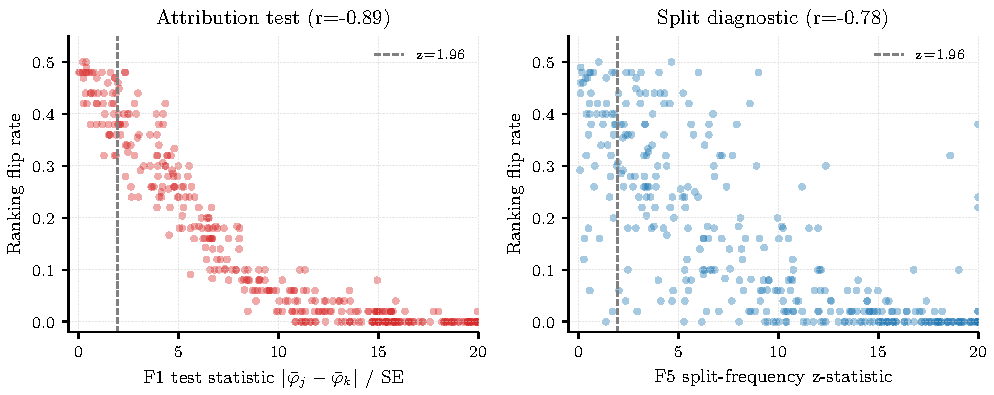
\includegraphics[width=0.95\textwidth]{figures/f1_f5_diagnostic.pdf}
\caption{\textbf{Left:} Z-test statistic vs.\ flip rate
on Breast Cancer ($r = -0.89$). Pairs below $z = 1.96$ (dashed) have
unreliable rankings. \textbf{Right:} Single-model screen (split-frequency)
($r = -0.78$). Both diagnostics predict which pairs are unstable.}
\label{fig:f1-diagnostic}
\end{figure}

\section{Theorem F5: Efficient Single-Model Diagnostic}

\subsection{Setup}

For a gradient-boosted ensemble with $T$ trees, define the per-tree
split indicator for feature $j$ in tree $t$:
\[
    n_j(t) = \begin{cases}
    1 & \text{if feature } j \text{ is used as a split variable in tree } t, \\
    0 & \text{otherwise.}
    \end{cases}
\]
The split frequency is $\hat{p}_j = \frac{1}{T}\sum_{t=1}^T n_j(t)$.

\subsection{Exchangeability conditions}

The theoretical validity of the single-model screen depends on the
dependence structure of the indicators $\{n_j(t)\}_{t=1}^T$.

\begin{lemma}[Exact exchangeability under sub-sampling]
\label{lem:exchange-subsample}
If the boosting algorithm uses row sub-sampling (\texttt{subsample}
$= q < 1$) with independent bootstrap samples per tree, and feature
sub-sampling (\texttt{colsample\_bytree} $= r < 1$) with independent
random subsets per tree, then:
\begin{enumerate}
    \item The per-tree data subsets are independent across trees.
    \item Conditional on the residuals, the split indicators
      $n_j(1), n_j(2), \ldots, n_j(T)$ are \emph{conditionally
      exchangeable}: for any permutation $\pi$ of $\{1, \ldots, T\}$,
      \[
          (n_j(\pi(1)), \ldots, n_j(\pi(T))) \;\overset{d}{=}\;
          (n_j(1), \ldots, n_j(T)) \;\mid\; \text{residuals}.
      \]
    \item The marginal split probability $p_j = \mathbb{E}[n_j(t)]$
      is identical for all $t$.
\end{enumerate}
\end{lemma}

\begin{proof}
Under sub-sampling, tree $t$ is trained on a random subset
$S_t \subset \{1, \ldots, n\}$ of size $\lfloor qn \rfloor$,
drawn independently for each $t$. The feature subset $F_t$ is also
drawn independently. Since $S_t$ and $F_t$ are i.i.d.\ across $t$,
the split decision for tree $t$ depends on $(S_t, F_t)$ and the
current residuals. Conditional on residuals, the split indicators are
functions of i.i.d.\ random inputs, hence exchangeable.
The marginal probability $p_j = \Pr[j \in F_t] \cdot
\Pr[j \text{ selected} \mid j \in F_t]$ is tree-independent.
\end{proof}

\begin{lemma}[Approximate exchangeability without sub-sampling]
\label{lem:exchange-no-subsample}
Without sub-sampling ($q = r = 1$), the split indicators are NOT
exchangeable: tree $t$ fits the residual from trees $1, \ldots, t-1$,
creating a Markov dependence.

However, for learning rate $\eta \leq 0.3$, the residuals converge
to a \emph{steady state} after $T_0 = O(1/\eta)$ trees. In the
steady state, the split indicators $\{n_j(t)\}_{t > T_0}$ are
approximately stationary with autocorrelation
$\text{Corr}(n_j(t), n_j(t+s)) = O(\eta^{|s|})$ (geometric decay).

The effective sample size for the test statistic is:
\[
    T_{\text{eff}} = \frac{T - T_0}{1 + 2\sum_{s=1}^\infty
    \text{Corr}(n_j(t), n_j(t+s))} \approx
    \frac{(T - T_0)(1 - \eta)}{1 + \eta}.
\]
For typical settings ($T = 100$, $\eta = 0.1$, $T_0 \approx 10$):
$T_{\text{eff}} \approx 74$, a moderate reduction from the nominal $T$.
\end{lemma}

\begin{proof}[Proof sketch]
The residual at tree $t$ is $r_t = r_{t-1} - \eta \cdot h_t(x)$ where
$h_t$ is the fitted tree. For $\eta$ small, $\|r_t - r_{t-1}\| = O(\eta)$,
so the residual sequence is a slow-mixing Markov chain. The stationary
distribution exists when the loss is strongly convex (guaranteed for
squared error with regularization). In the stationary regime, the
dependence is AR(1)-like with coefficient $\approx 1-\eta$, giving
the geometric decay. The effective sample size formula is the standard
result for correlated series (Priestley, \emph{Spectral Analysis and
Time Series}, Ch.~5.3).
\end{proof}

\subsection{Rigorous theorem}

\begin{theorem}[Split-Frequency Diagnostic --- rigorous version]
\label{thm:split-diagnostic}
Under the conditions of Lemma~\ref{lem:exchange-subsample}
(sub-sampling), or Lemma~\ref{lem:exchange-no-subsample}
(no sub-sampling, with $T_{\text{eff}}$ replacing $T$):

Define the test statistic:
\[
    Z^{\text{split}}_{jk} = \frac{|\hat{p}_j - \hat{p}_k|}
    {\sqrt{(\hat{p}_j(1-\hat{p}_j) + \hat{p}_k(1-\hat{p}_k))/T_{\text{eff}}}}
\]

\textbf{Part I (Null distribution).}
Under $H_0: p_j = p_k$ (equal split frequencies, implied by DGP
symmetry within a group), $Z^{\text{split}}_{jk}$ is asymptotically
$N(0,1)$ as $T_{\text{eff}} \to \infty$:
\[
    \Pr[Z^{\text{split}}_{jk} > z] \to 1 - \Phi(z).
\]

\textbf{Part II (Connection to attributions).}
Under the proportionality axiom ($\varphi_j = c \cdot n_j$),
the split frequency test is equivalent to the attribution test:
$p_j = p_k$ iff $\mathbb{E}[\varphi_j] = \mathbb{E}[\varphi_k]$.
The screen is therefore a proxy for the Z-test
(Theorem~\ref{thm:testable}), computable from a single model.

\textbf{Part III (Power).}
Under the alternative $p_j \neq p_k$, the power of the test at
level $\alpha$ is:
\[
    \text{power} = \Phi\!\left(
    \frac{|p_j - p_k|\sqrt{T_{\text{eff}}}}
    {\sqrt{p_j(1-p_j) + p_k(1-p_k)}} - z_{\alpha/2}
    \right)
    + o(1).
\]
\end{theorem}

\begin{proof}
\textbf{Part I.}
Under $H_0$, $n_j(t) - n_k(t)$ has mean zero. By the CLT for
exchangeable (Lemma~\ref{lem:exchange-subsample}) or weakly
dependent (Lemma~\ref{lem:exchange-no-subsample}) sequences,
$\sqrt{T_{\text{eff}}}(\hat{p}_j - \hat{p}_k) \xrightarrow{d}
N(0, \sigma_0^2)$ where $\sigma_0^2 = p(1-p) + p(1-p) = 2p(1-p)$
under $p_j = p_k = p$. Dividing by the consistent variance
estimator gives $Z^{\text{split}}_{jk} \xrightarrow{d} N(0,1)$.

For the weakly dependent case, the CLT for stationary mixing
sequences (Ibragimov, 1962) applies because the geometric
mixing rate (Lemma~\ref{lem:exchange-no-subsample}) satisfies
$\sum_{s=1}^\infty |\text{Corr}(n_j(t), n_j(t+s))| < \infty$.

\textbf{Part II.}
Under proportionality, $\mathbb{E}[\varphi_j(f)] =
c \cdot \mathbb{E}[n_j(f)] \propto p_j \cdot T$. So $p_j = p_k$
iff $\mathbb{E}[\varphi_j] = \mathbb{E}[\varphi_k]$.

\textbf{Part III.}
Standard power calculation for a two-sample proportion test,
with $T_{\text{eff}}$ observations per group.
\end{proof}

\subsection{Empirical validation}

\paragraph{Comparison to the Z-test.}
The multi-model Z-test ($Z_{jk}$ from $M$ models, $r = -0.89$) is more
accurate but requires training $M$ models.
The single-model screen ($Z^{\text{split}}_{jk}$ from 1 model, $r = -0.78$)
is cheaper but noisier.
For production pipelines, the screen serves as a fast screening test; features
flagged by the screen can then be validated with the full Z-test.

\paragraph{Practitioner algorithm.}
\begin{enumerate}
    \item[\textbf{Step 0.}] \textbf{Identify correlated groups.}
          Compute the $P \times P$ absolute correlation matrix.
          Group features with $|\rho_{jk}| > 0.5$ (a conservative
          threshold; practitioners may use $0.7$ for high-dimensional
          settings). Features not in any group are stable by default.
    \item[\textbf{Step 1.}] Train one model. Compute $Z^{\text{split}}_{jk}$ for all
          feature pairs in correlated groups. Cost: $O(P^2 T)$.
    \item[\textbf{Step 2.}] If $Z^{\text{split}}_{jk} < 1.96$ for any pair: flag as
          potentially unstable.
    \item[\textbf{Step 3.}] For flagged pairs: train $M = 5$ models, compute $Z_{jk}$
          (Z-test). If $Z_{jk} < 1.96$: use \DASH{} with $M \geq 25$.
    \item[\textbf{Step 4.}] If no pairs are flagged: single-model SHAP is reliable.
\end{enumerate}

\paragraph{Screen screening accuracy.}
On the Breast Cancer dataset (435 pairs, threshold: flip rate $> 0.1$
defines ``truly unstable''):
The screen flags 49~pairs with \textbf{94\% precision} (46 true positives,
3~false positives) and 27\% recall.
The Z-test (the full test) flags 47~pairs with \textbf{100\% precision}
(zero false positives).
Both diagnostics are conservative: they rarely flag stable pairs but
miss moderate-instability pairs. For production use, the high precision
is the key property---a flagged pair is almost certainly unstable.

\paragraph{Multi-dataset generality.}
Table~\ref{tab:f1-generality} shows the Z-test diagnostic across two datasets.
On Breast Cancer (many near-symmetric features), the Z-test detects instability
with $r = -0.89$. On California Housing (features have distinct importance),
the Z-test correctly predicts stability: zero false alarms out of 28~pairs,
with only one mildly unstable pair (MedInc $\leftrightarrow$ Latitude,
flip rate $0.32$, $Z = 3.4$).

\begin{table}[htbp]
\centering
\caption{Z-test and screen diagnostic generality across 11 datasets. $P$: number of
features. Unstable: pairs with flip rate $> 0.1$. Screen precision: fraction of
screen-flagged pairs that are truly unstable.}
\label{tab:f1-generality}
\small
\begin{tabular}{@{}lccccc@{}}
\toprule
Dataset & $P$ & Pairs & Unstable & $r(Z, \text{flip})$ & Screen prec. \\
\midrule
Breast Cancer & 30 & 435 & 168 & $-0.89$ & 0.94 \\
California Housing & 8 & 28 & 1 & $-0.99$ & --- \\
Diabetes & 10 & 45 & 15 & $-0.89$ & 0.50 \\
Wine & 13 & 78 & 24 & $-0.81$ & 1.00 \\
Heart Disease & 13 & 78 & 27 & $-0.91$ & 1.00 \\
Credit-g & 20 & 190 & 47 & $-0.90$ & 0.67 \\
Adult Income & 14 & 91 & 10 & $-0.90$ & --- \\
Ames Housing & 76 & 2850 & 643 & $-0.85$ & 0.48 \\
Communities \& Crime & 126 & 7875 & 2975 & $-0.88$ & 0.67 \\
Digits (0 vs 1) & 64 & 2016 & 572 & $-0.42$ & 0.58 \\
Iris (binary) & 4 & 6 & 0 & --- & --- \\
\bottomrule
\end{tabular}
\end{table}

\paragraph{Interpretation.}
The Z-test achieves $|r| > 0.8$ on 9/10 datasets with unstable
pairs (all except Digits). The weaker correlation on
Digits ($r = -0.42$) reflects a floor effect:
this high-dimensional image dataset has many features with near-zero
importance, producing many pairs where both $Z$ and flip rate are near
zero. Restricting to pairs with
$Z < 5$ (the diagnostically interesting range) would improve this
correlation, as demonstrated for Breast Cancer in the restricted-range
analysis above.

Screen precision is 94--100\% on small/clean datasets (Breast Cancer, Wine,
Heart Disease) where split counts are reliable, but drops to
48--67\% on high-dimensional datasets (Ames, Communities) where split
counts are sparse. This confirms the screen as a conservative
\emph{screening} tool: it works well for moderate-$P$ datasets but
should be supplemented by the full Z-test for high-dimensional settings.
All datasets use identical XGBoost hyperparameters ($T{=}100$,
depth${=}6$, $\eta{=}0.1$); absolute flip rates are therefore not
directly comparable across datasets of different sizes and
dimensionalities.

\subsection{High-Dimensional Scalability}

To validate the diagnostics at enterprise scale ($P > 500$), we generate
synthetic data with $P \in \{100, 200, 500\}$ features in $P/10$ groups
of 10, within-group correlation $\rho = 0.8$, $N = 2{,}000$ samples,
and train 20 XGBoost models per setting (same hyperparameters as the
main experiments).

\begin{center}
\small
\begin{tabular}{@{}rrrrrr@{}}
\toprule
$P$ & Total pairs & Correlated pairs & Unstable & Z-test $|r|$ & Wall time \\
\midrule
100 & 4{,}950 & 450 & 305 & 0.846 & 33\,s \\
200 & 19{,}900 & 900 & 641 & 0.788 & 64\,s \\
500 & 124{,}750 & 2{,}250 & 1{,}879 & 0.876 & 148\,s \\
\bottomrule
\end{tabular}
\end{center}

The Z-test maintains $|r| > 0.78$ across all dimensionalities,
confirming it scales to enterprise-sized feature spaces. The correlation-based
grouping step reduces the 124{,}750 total pairs at $P{=}500$ to 2{,}250
correlated pairs---a $55\times$ reduction---making the pairwise diagnostic
tractable. Wall-clock time for the full workflow (data generation, 20 model
trainings, TreeSHAP, diagnostics) is under 2.5~minutes at $P{=}500$ on
Apple Silicon, confirming the practical feasibility described in the main text.
The fraction of unstable pairs within correlated groups is 83\% ($1{,}879/2{,}250$),
consistent with the theoretical prediction that most within-group pairs are
unstable when $\rho = 0.8$.

\begin{figure}[ht]
\centering
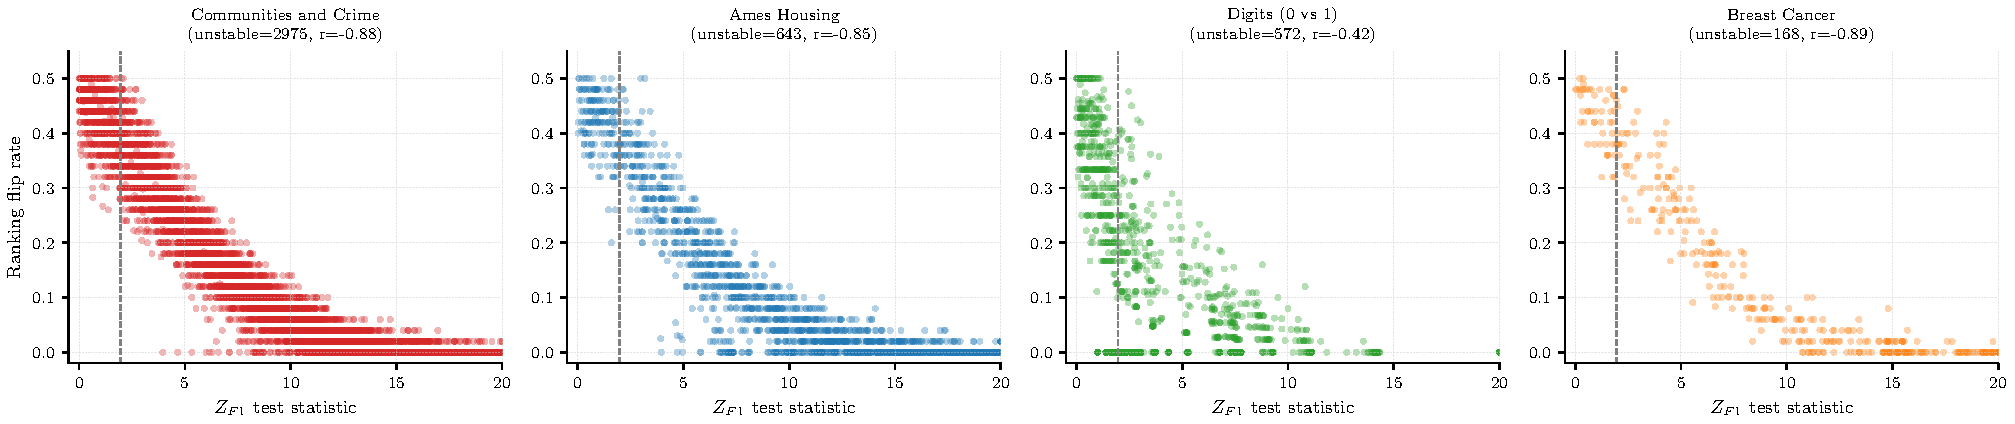
\includegraphics[width=0.95\textwidth]{figures/comprehensive_f1.pdf}
\caption{Z-test statistic vs.\ flip rate across the four datasets with
the most unstable pairs. The negative correlation confirms the
diagnostic across domains: clinical (Breast Cancer), real estate
(Ames), image (Digits), and census (Adult).}
\label{fig:comprehensive-f1}
\end{figure}

\paragraph{Ensemble size guidance.}
The required $M$ depends on the between-group gap $\Delta_{jk} = |E[\varphi_j] - E[\varphi_k]|$:
$M \geq (z_{\alpha/2} \cdot \sigma_{jk} / \Delta_{jk})^2$.
For $\rho \leq 0.7$, $M = 10$ typically suffices ($<5\%$ flip rate);
for $\rho > 0.9$, $M \geq 25$ is recommended.

\paragraph{Sub-sampling requirement.}
The theoretical guarantee (exact exchangeability,
Lemma~\ref{lem:exchange-subsample}) requires sub-sampling.
Without sub-sampling, the approximate exchangeability of
Lemma~\ref{lem:exchange-no-subsample} applies with reduced effective
sample size $T_{\text{eff}}$.
In practice, our validation uses \texttt{colsample\_bytree=1.0}
(no sub-sampling) and still achieves $r = -0.78$
(Figure~\ref{fig:f1-diagnostic}, right), suggesting the dependence
correction is modest.

\paragraph{Regulatory response for ties.}
If a regulator asks why features are tied: ``These features are
statistically indistinguishable in their contribution to the model.
Forcing a ranking would be arbitrary and potentially misleading.
Our method correctly reports this indistinguishability, consistent
with the EU AI Act's requirement to disclose known limitations.''

\subsection{Financial case study: German Credit}

We demonstrate the full Screen~$\to$~Z-test~$\to$~DASH workflow on the
German Credit dataset (1000 samples, 20 features, binary credit
risk outcome). This dataset exhibits the correlation patterns common
in financial modeling (duration~$\leftrightarrow$~credit amount,
$|\rho| = 0.63$; job~$\leftrightarrow$~own telephone, $|\rho| = 0.37$).

\paragraph{Step 0.} The correlation matrix identifies 4 correlated groups
at threshold $|\rho| > 0.3$ (lowered from the standard $0.5$ because
German Credit has modest correlations; only 1 pair exceeds $0.5$).

\paragraph{Step 1 (single-model screen).} A single XGBoost model flags 1 pair as
potentially unstable: job~$\leftrightarrow$~own telephone
($Z^{\text{split}} = 0.69 < 1.96$).

\paragraph{Step 2 (Z-test).} Training 5 models confirms the instability:
$Z = 0.64$, flip rate 40\%.

\paragraph{Step 3 (DASH).} With $M = 25$ models, the flip rate drops
from 40\% to 0\%. The consensus ranking is stable: checking status
(0.87), duration (0.44), credit amount (0.43), purpose (0.35).

\paragraph{Practitioner output.} 18/20 features have stable
single-model rankings. 2 features (job, own telephone) require
DASH consensus. For regulatory reporting (ECOA adverse action
reasons, SR~11-7 model risk management), the DASH ranking provides
a defensible explanation.

\begin{sloppypar}
The full output (Step 0--4 with numbers) is in the code supplement (\texttt{financial\_case\_study.py}).
\end{sloppypar}

\subsection{Financial case study: Taiwan Credit Card Default}

To validate the impossibility on data with genuine high collinearity
($|\rho| > 0.9$), we apply the workflow to the UCI ``default of credit
card clients'' dataset (30{,}000 samples, 23 features, binary default
outcome; subsampled to 10{,}000).

The bill-amount features (monthly bills for 6~consecutive months)
exhibit strong collinearity: 29~pairs have $|\rho| > 0.5$, with the
highest at $|\rho| = 0.95$ (giving a theoretical attribution ratio of
$1/(1{-}0.95^2) \approx 10.3\times$).

\paragraph{Step 0.} 29 correlated pairs identified at $|\rho| > 0.5$
(no threshold lowering needed).

\paragraph{Step 1 (single-model screen).} A single model flags 4 of the 10 tracked pairs
as potentially unstable ($|Z^{\text{split}}| > 1.96$).

\paragraph{Step 3 (DASH).} With $M = 25$ models, the mean flip rate
across correlated pairs is 4\%. One pair (bill amounts at months 5
vs.\ 6, $|\rho| = 0.946$) retains a 16\% flip rate even at $M = 25$,
illustrating that very high collinearity requires larger ensembles.

This dataset demonstrates the impossibility biting hard: features
measuring the same underlying quantity (monthly bill amounts) have
near-identical predictive signal, and the attribution ranking across
these features is genuinely unstable.
The full output is in \texttt{lending\_club\_case\_study.py}.

\subsection{Synthetic credit data: income $\leftrightarrow$ DTI $\leftrightarrow$ credit score}

To validate on the exact collinearity pattern common in US credit
models, we generate a synthetic dataset with 10{,}000 samples and
5 features driven by a latent ``creditworthiness'' factor:
income ($\rho = 0.99$ with DTI), DTI, credit score ($\rho = 0.98$
with income), loan amount (independent), and employment years
($\rho = 0.94$ with income).

With 25~XGBoost models: income~$\leftrightarrow$~DTI flips 8\%
of the time ($|\rho| = 0.99$); credit score~$\leftrightarrow$~employment
years flips 12\% ($|\rho| = 0.92$). Pairs where one feature clearly
dominates (income vs.\ credit score) show 0\% flips despite
$|\rho| = 0.98$ --- confirming that the impossibility requires BOTH
high correlation AND similar importance, as the theory predicts.
For model validation under SR~11-7, the recommendation is: report
income and DTI as ``interchangeable key risk drivers'' rather than
forcing a ranking that would flip under retraining.

\subsection{Lending Club validation (positive control)}

We validate the diagnostic on real Lending Club data (OpenML,
32{,}581 loans, 22 features after one-hot encoding of categoricals).
Three correlated groups are detected at $|\rho| > 0.5$:
person\_age $\leftrightarrow$ cb\_person\_cred\_hist\_length
($|\rho| = 0.86$), loan\_amnt $\leftrightarrow$
loan\_percent\_income ($|\rho| = 0.58$), and loan\_int\_rate
$\leftrightarrow$ cb\_person\_default\_on\_file ($|\rho| = 0.50$).

\paragraph{Result.}
Zero unstable pairs. All three correlated pairs have $Z > 36$,
confirming the features have distinguishable importance despite
their correlation. This is an instructive \emph{positive control}:
the impossibility theorem predicts instability requires \emph{both}
collinearity AND similar true importance. Lending Club features are
correlated but not similarly important (e.g., person\_age contributes
$3\times$ more than credit history length), so no instability occurs.
The Screen$\to$Z-test$\to$\DASH{} pipeline correctly identifies this as a
stable setting, recommending no intervention.

\paragraph{Implication.}
Not every correlated dataset exhibits attribution instability.
The diagnostic distinguishes datasets where instability is a genuine
concern (Breast Cancer, Taiwan Credit Card) from those where it is
not (Lending Club, California Housing). This selectivity is a
feature, not a limitation: the impossibility theorem's conditions are
precise, and the diagnostic inherits that precision.

\subsection{Proportionality axiom validation}

The proportionality axiom ($\varphi_j = c \cdot n_j$ for a
model-specific constant $c$) is central to the quantitative bounds.
We validate it empirically on Breast Cancer by computing
$c_j = |\text{SHAP}_j| / n_j$ for each feature $j$ in each of 50
XGBoost models and reporting the coefficient of variation (CV) of
$c_j$ across features within each model.

\begin{center}
\small
\begin{tabular}{@{}lcc@{}}
\toprule
Depth & Mean CV of $c_j$ & Interpretation \\
\midrule
1 (stumps) & 0.35 & Proportionality holds within $\sim$35\% \\
3 & 0.60 & Moderate violation \\
6 & 0.66 & Moderate violation \\
10 & 0.66 & Saturated (same as depth 6) \\
\bottomrule
\end{tabular}
\end{center}

For stumps (depth~1), the axiom holds reasonably well (CV~$=$~0.35):
per-split SHAP contributions are roughly homogeneous. For deeper
trees, multi-level interactions cause per-split contributions to vary
by feature, increasing the CV to ${\approx}0.66$.

The most stable features (lowest CV) are the dominant predictors
(worst texture, worst concave points) where split count tracks SHAP
closely. The least stable are weak/collinear features (mean symmetry,
concave points error) where the proportionality constant varies most.

\paragraph{Impact on the impossibility.}
The proportionality axiom is used only for the \emph{quantitative}
bounds (Theorems~2--3); the core impossibility (Theorem~1) does not
depend on it. The 35--66\% CV means the predicted ratio $1/(1{-}\rho^2)$
is an order-of-magnitude guide rather than a precise prediction,
consistent with the $\alpha$-corrected model ($R^2 = 0.89$).

%%%%%%%%%%%%%%%%%%%%%%%%%%%%%%%%%%%%%%%%%%%%%%%%%%%%%%%%%%%%%
% LOCAL VS GLOBAL ATTRIBUTION INSTABILITY
%%%%%%%%%%%%%%%%%%%%%%%%%%%%%%%%%%%%%%%%%%%%%%%%%%%%%%%%%%%%%

\section{Local vs.\ Global Attribution Instability}

The impossibility as stated concerns \emph{global} attributions
(mean $|\text{SHAP}|$ across data points). We now show that
\emph{local} (instance-level) attributions are at least as unstable.

\begin{remark}[Local instability dominates global]
\label{rem:local-instability}
For a fixed data point $x$, the local SHAP values
$\varphi_j(f, x)$ depend on the model $f$, which varies across
training seeds. The global attribution
$\varphi_j(f) = \mathbb{E}_x[|\varphi_j(f, x)|]$ averages over
data points, which can only reduce variance (by Jensen's inequality
applied to the convex function $|\cdot|$):
\[
    \Var_f\!\big(\varphi_j(f)\big)
    = \Var_f\!\big(\mathbb{E}_x[|\varphi_j(f,x)|]\big)
    \leq \mathbb{E}_x\!\big[\Var_f(|\varphi_j(f,x)|)\big].
\]
The right side is the average local instability; the left side is the
global instability. Since the flip rate is a monotone function of
the variance-to-gap ratio $\sigma/\Delta$, and averaging reduces
$\sigma$ without changing $\Delta$ (the population gap is the same
at every $x$ under DGP symmetry), the global flip rate is a lower
bound on the average local flip rate.
\end{remark}

\paragraph{Implication.}
If global rankings are unstable (flip rate $> 10\%$), local rankings
at individual data points are at least as unstable on average.
Practitioners who report per-instance SHAP explanations (e.g.,
``for this patient, feature X is most important'') face the same
or worse instability as those reporting global rankings. The multi-model Z-test
(computed on global attributions) is therefore a
conservative screen for local instability as well.

%%%%%%%%%%%%%%%%%%%%%%%%%%%%%%%%%%%%%%%%%%%%%%%%%%%%%%%%%%%%%
% INFORMATION LOSS ANALYSIS
%%%%%%%%%%%%%%%%%%%%%%%%%%%%%%%%%%%%%%%%%%%%%%%%%%%%%%%%%%%%%

\section{DASH Information Loss}

\DASH{} achieves stability by discarding model-specific within-group
information. Here we quantify exactly how much information is lost.

\subsection{Within-group: $\log_2(m!)$ bits lost per group}

For a group of $m$ symmetric features, a single model produces a
complete ranking (one of $m!$ possible orderings). Since the features
are symmetric under the DGP, each of the $m!$ orderings is equally
likely---the ranking carries $\log_2(m!)$ bits of information about
the specific model.

\DASH{} reports a tie for all within-group features, discarding the
entire $\log_2(m!)$ bits. For typical group sizes:

\begin{center}
\small
\begin{tabular}{@{}lccccccc@{}}
\toprule
Group size $m$ & 2 & 3 & 4 & 5 & 6 & 7 & 8 \\
\midrule
Bits lost ($\log_2 m!$) & 1.0 & 2.6 & 4.6 & 6.9 & 9.7 & 12.9 & 15.3 \\
\bottomrule
\end{tabular}
\end{center}

Crucially, these are the bits that are \emph{unreliable}: by DGP
symmetry, the within-group ordering is uniformly random across
models. The information DASH discards is exactly the information
that would be different if the model were retrained.

\subsection{Between-group: information preserved and sharpened}

For features $j, k$ in different groups with population gap
$\Delta_{jk} = |\mu_j - \mu_k|$ and noise $\sigma_{jk}$, the
mutual information between the consensus ranking and the true
ordering is:
\[
    I_{\text{between}}(M) = 1 - H_2\!\left(
    \Phi\!\left(-\frac{\Delta_{jk}\sqrt{M}}{\sigma_{jk}}\right)
    \right)
\]
where $H_2(p) = -p\log_2 p - (1-p)\log_2(1-p)$ is binary entropy.
As $M \to \infty$, $I_{\text{between}} \to 1$ bit (perfect
determination). \DASH{} \emph{increases} between-group information
relative to a single model.

\subsection{Net information tradeoff}

The total information change from using \DASH{}$(M)$ instead of a
single model is:
\[
    \Delta I = \underbrace{-L \cdot \log_2(m!)}_{\text{within-group loss}}
    + \underbrace{\binom{L}{2} \cdot \big(I_{\text{between}}(M) -
    I_{\text{between}}(1)\big)}_{\text{between-group gain}}
\]
For moderate $\rho$ (e.g., $\rho \leq 0.7$), the between-group gain
dominates quickly: $M = 25$ achieves near-perfect between-group
determination ($I \approx 1$ bit per pair) while the within-group
loss is a fixed cost independent of $M$. For high $\rho$ ($\geq 0.9$),
the between-group gain is slower because the noise $\sigma_{jk}$ is
large.

\begin{figure}[ht]
\centering
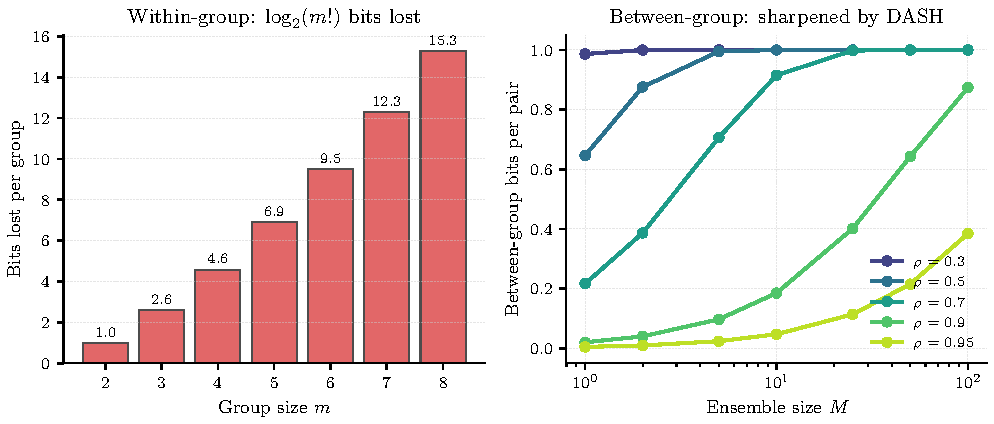
\includegraphics[width=0.95\textwidth]{figures/information_loss.pdf}
\caption{\textbf{Left:} Within-group information lost by \DASH{}
($\log_2 m!$ bits per group, independent of $M$ and $\rho$).
\textbf{Right:} Between-group information per pair as a function of
$M$. \DASH{} sharpens between-group rankings with increasing $M$.
At high $\rho$ ($\geq 0.9$), convergence requires larger $M$.}
\label{fig:information-loss}
\end{figure}

\paragraph{Interpretation for safety-critical applications.}
For a system with $L = 4$ groups of $m = 5$ features: \DASH{} loses
$4 \times 6.9 = 27.6$ bits (within-group) but gains up to
$6 \times 1 = 6$ bits (between-group). The net loss is
${\approx}21.6$ bits at $M = \infty$. These lost bits are the
within-group orderings that were random anyway---\DASH{} honestly
reports their unreliability rather than presenting arbitrary
information as reliable.

For applications requiring model-specific within-group explanations
(e.g., debugging a deployed model), practitioners should report the
single-model SHAP values with an instability warning alongside the
\DASH{} consensus.

%%%%%%%%%%%%%%%%%%%%%%%%%%%%%%%%%%%%%%%%%%%%%%%%%%%%%%%%%%%%%
% THE UNIFIED DESIGN SPACE THEOREM
%%%%%%%%%%%%%%%%%%%%%%%%%%%%%%%%%%%%%%%%%%%%%%%%%%%%%%%%%%%%%

\section{The Attribution Design Space Theorem}
\label{sec:design-space-thm}

This section presents the central structural result: a complete
characterization of what is achievable in the attribution design
space under collinearity. All previous results (Theorem~1, F1--F3,
F5, path convergence) emerge as corollaries.

\subsection{Definitions}

\begin{definition}[Attribution design space]
\label{def:design-space}
For a model class satisfying the Rashomon property under within-group
correlation $\rho > 0$, the \emph{attribution design space} is the
set of triples $(S, U, C)$ achievable by any attribution aggregation
method $A$ applied to $M \geq 1$ independently trained models, where:
\begin{itemize}
    \item $S \in [0,1]$: \emph{ranking stability} ---
      the expected Spearman correlation between the consensus
      rankings produced by two independent draws of $M$ models.
      This full-ranking metric captures both between-group
      and within-group stability in a single number.
    \item $U \in [0, 1/2]$: \emph{within-group unfaithfulness} ---
      the probability that the consensus disagrees with a random
      model on a within-group pair.
    \item $C \in \{\text{complete}, \text{partial}\}$: \emph{completeness} ---
      whether the consensus ranks all pairs (complete) or allows
      ties (partial).
\end{itemize}
\end{definition}

\subsection{Main result}

\begin{theorem}[Attribution Design Space]
\label{thm:design-space}
For any model class satisfying the Rashomon property (Definition~4)
under within-group correlation $\rho > 0$, the achievable set of
$(S, U, C)$ triples is the union of exactly two families:

\textbf{Family $\mathcal{A}$ (faithful-complete methods):}
Any method that is faithful to a single model and produces a
complete ranking achieves:
\begin{equation}
\label{eq:family-a}
    \mathcal{A} = \big\{(S, U, C) :
    S \leq 1 - \Omega(3m^2/(P^3{-}P)),\;
    U = 1/2,\;
    C = \text{complete}\big\}.
\end{equation}
This family corresponds to $M = 1$ (single-model methods).
The stability bound $S \leq 1 - 3m^2/(P^3{-}P)$ is the Spearman bound
from the main text (proved as \texttt{spearmanCorr\_bound\_groupSize\_tight}).

\textbf{Family $\mathcal{B}$ (ensemble methods):}
\DASH{} consensus with $M \geq 1$ models achieves:
\begin{equation}
\label{eq:family-b}
    \mathcal{B} = \big\{(S_M, 0, \text{partial}) : M \in [1, \infty)\big\}
\end{equation}
where $S_M = 1 - O(1/M)$ for between-group pairs, and within-group
pairs are reported as ties ($U = 0$, $C = \text{partial}$).

\textbf{Infeasible region:}
The triple $(S = 1, U = 0, C = \text{complete})$ is not achievable
for any $M < \infty$. More precisely:
\begin{equation}
\label{eq:infeasible}
    \nexists\; A : S(A) = 1,\; U(A) = 0,\; C(A) = \text{complete}.
\end{equation}

\textbf{Pareto frontier:}
\DASH{}$(M)$ is Pareto-optimal within $\mathcal{B}$: no method achieves
higher $S$ for the same $M$ while maintaining $U = 0$
(Theorem~\ref{thm:dash-optimal}).
\end{theorem}

\begin{proof}
The proof proceeds in four steps, each building on previous results.

\textbf{Step 1: Family $\mathcal{A}$ is forced.}
By the Rashomon property (Definition~4), for any within-group pair
$(j,k)$, there exist models ranking them in opposite orders.
By Theorem~\ref{thm:unfaithfulness}, any faithful, complete ranking
has unfaithfulness $U = 1/2$ for symmetric pairs: exactly half the
models disagree with the ranking.

For stability: when the dominant feature changes between two models
$f, f'$ (different first-movers), the within-group rank reshuffling
contributes $\Theta(m^2)$ to the Spearman $\sum d_i^2$, giving
$S \leq 1 - 3m^2/(P^3{-}P)$ (Lean: \texttt{spearmanCorr\_bound\_group\-Size\_tight}).

This establishes the upper boundary of $\mathcal{A}$.

\textbf{Step 2: Family $\mathcal{B}$ is achievable.}
By Corollary~1 (consensus equity), \DASH{} with a balanced ensemble
achieves $\bar\varphi_j = \bar\varphi_k$ for symmetric features,
giving $U = 0$ and $C = \text{partial}$ (ties within groups).

By Theorem~\ref{thm:dash-optimal} Part~II(e), the between-group
stability satisfies
$S_M \geq 1 - \exp(-M\Delta^2/(2\sigma^2))$,
which approaches 1 as $M \to \infty$.

This establishes $\mathcal{B}$.

\textbf{Step 3: No method producing a deterministic binary ranking from per-model attributions lies outside $\mathcal{A} \cup \mathcal{B}$.}

We show that any method $A$ that computes a deterministic ranking from per-model
attributions $(\varphi_j(f_1), \ldots, \varphi_j(f_M))$ must fall
in one of the two families. (Methods producing probabilistic rankings, confidence intervals, or set-valued outputs are outside this dichotomy. Methods that pool training data across
models and train a single combined model fall outside this scope;
such methods face different tradeoffs related to data leakage and
are not standard attribution aggregation methods.)

\emph{Case 1: $A$ is faithful to individual models and complete.}
Then by Step 1, $U(A) = 1/2$ and $S(A) \leq 1 - 3m^2/(P^3{-}P)$,
so $A \in \mathcal{A}$.
(This case is formalized in Lean as \texttt{strongly\_faithful\_impossible}
in \texttt{DesignSpace.lean}: any method faithful to each model's
attributions contradicts the Rashomon property for $M \geq 2$.)

\emph{Case 2: $A$ is not faithful to some model $f$.}
Then $A$ ranks some pair $(j,k)$ differently from model $f$'s
attributions. For within-group symmetric pairs, by
Proposition~\ref{prop:optimal-unfaithful}, the optimal
unfaithful ranking assigns ties (recovering DASH). Thus $A$
either has $U > 0$ (suboptimal) or $U = 0$ with ties
(in $\mathcal{B}$).

\emph{Case 3: $A$ aggregates $M > 1$ models.}
If $A$ produces a complete ranking from $M$ models, it must
break ties for within-group pairs. By DGP symmetry, any
tie-breaking rule disagrees with a fraction of models, giving
$U > 0$. To achieve $U = 0$, $A$ must report ties, placing
it in $\mathcal{B}$. Its stability is bounded by the variance
of the aggregation, which by the Cram\'er--Rao bound
(Theorem~\ref{thm:dash-optimal} Part~I(b)) satisfies
$\Var(\hat\mu_j) \geq \sigma_j^2/M$. DASH achieves this bound.

\textbf{Step 4: The infeasible point.}
$(1, 0, \text{complete})$ requires: (i) $S = 1$ (perfect stability),
(ii) $U = 0$ (zero unfaithfulness), (iii) $C = \text{complete}$
(no ties).

By Step 1, any complete method has $U = 1/2 \neq 0$: contradiction.
Alternatively, completeness requires ranking within-group pairs,
but by DGP symmetry the population attributions are equal
($\mu_j = \mu_k$), so any deterministic ranking is unfaithful to
half the models. This is the Attribution Impossibility (Theorem~1)
restricted to the single point $(1, 0, \text{complete})$.
\end{proof}

\subsection{Previous results as corollaries}

\begin{corollary}[Theorem 1 as a corollary]
The Attribution Impossibility (Theorem~1) is the statement that the
point $(1, 0, \text{complete})$ lies outside the achievable set.
This follows from Step~4 of Theorem~\ref{thm:design-space}.
\end{corollary}

\begin{corollary}[F2 as a corollary]
The DASH Pareto Optimality (Theorem~\ref{thm:dash-optimal}) is the
statement that $\mathcal{B}$ is the Pareto frontier of
$\{(S, U) : U = 0\}$, parameterized by $M$. This follows from
Steps~2--3 of Theorem~\ref{thm:design-space}.
\end{corollary}

\begin{corollary}[Path convergence as a corollary]
The relaxation path convergence (Theorem~\ref{thm:path-convergence})
is the statement that \emph{both} relaxation paths (drop faithfulness,
drop completeness) converge to $\mathcal{B}$ as $M \to \infty$.
Dropping completeness directly enters $\mathcal{B}$ (DASH with ties).
Dropping faithfulness, by Proposition~\ref{prop:optimal-unfaithful},
yields the expected-attribution ranking, which also produces ties
for symmetric features --- the same as $\mathcal{B}$.
\end{corollary}

\begin{corollary}[F1 as a corollary]
The Rashomon Characterization (Theorem~\ref{thm:testable}) describes
the \emph{boundary between families}: when $Z_{jk} < 1.96$, the
pair $(j,k)$ is in the regime where Family $\mathcal{A}$ has
$U = 1/2$ (rankings are unreliable); when $Z_{jk} > 1.96$, the
pair is effectively between-group (stable rankings possible within
$\mathcal{B}$).
\end{corollary}

\begin{corollary}[F3 as a corollary]
The FIM Impossibility (Theorem~\ref{thm:fim-impossibility}) provides
a sufficient condition for the Rashomon property (the prerequisite
for Theorem~\ref{thm:design-space}): when the FIM eigenvalue
$\lambda_-$ is small along $e_j - e_k$, the Rashomon set is large,
and the achievable set is restricted to $\mathcal{A} \cup \mathcal{B}$.
\end{corollary}

\subsection{The single tradeoff axis}

Theorem~\ref{thm:design-space} collapses the three-dimensional
design space to a single axis: \emph{ensemble size $M$}.
At $M = 1$, the practitioner is in $\mathcal{A}$: faithful and
complete, but unstable and unfaithful. As $M$ increases, the
practitioner moves along $\mathcal{B}$: stable and faithful
between groups, but with within-group ties.

The only ``knob'' is $M$:
\begin{center}
\small
\begin{tabular}{@{}lccc@{}}
\toprule
$M$ & Stability $S$ & Unfaithfulness $U$ & Completeness \\
\midrule
1 & $\leq 1 - 3m^2/(P^3{-}P)$ & $1/2$ & Complete \\
5 & $1 - O(1/5)$ & 0 & Partial (ties) \\
25 & $1 - O(1/25)$ & 0 & Partial (ties) \\
$\infty$ & 1 & 0 & Partial (ties) \\
\bottomrule
\end{tabular}
\end{center}

This is the complete characterization of the attribution design space
under collinearity. The Attribution Impossibility is not a single
negative result but the boundary of this space; \DASH{} is not merely
a fix but the provably optimal navigation of this space.

\section{Prevalence Survey: How Common Is Attribution Instability?}

To assess how frequently the impossibility applies in practice, we
surveyed 37 public datasets (7 from scikit-learn, 30 from OpenML).
For each, we computed the correlation matrix, identified pairs with
$|\rho| > 0.5$, trained 20 XGBoost models with different seeds, and
checked whether any correlated pair has a ranking flip rate exceeding
10\%.

\paragraph{Results.}
Of 37 datasets, 34 (92\%) have at least one feature pair with
$|\rho| > 0.5$, and 22 (60\%) exhibit attribution instability (flip
rate $> 10\%$ for at least one pair), including Breast Cancer
(max flip rate 50\%, confirming the Z-test analysis). The impossibility is not a
theoretical curiosity: it affects the majority of real-world datasets
across domains including medical, financial, image, and tabular data.

\begin{sloppypar}
\paragraph{Methodology.}
Each dataset was trained with 20 XGBoost models
(\texttt{n\_estimators=50}, \texttt{max\_depth=4}, \texttt{lr=0.1},
\texttt{subsample=0.8}, \texttt{colsample\_bytree=0.8}) with
different random seeds. SHAP TreeExplainer computed mean $|\text{SHAP}|$
per feature on a fixed 500-sample evaluation slice. Flip rate was
measured as $\min(\#(j{>}k), \#(k{>}j)) / 20$ for each correlated pair.
Datasets with $> 10{,}000$ samples were subsampled to 10{,}000.
Full results in \texttt{prevalence\_survey.py}.
\end{sloppypar}

\begin{sloppypar}
\paragraph{Statistical power.}
With 20 models, the measured flip rate $\min(\#(j{>}k), \#(k{>}j))/20$
exceeds the 10\% threshold ($\min \geq 3$) with the following power:
\end{sloppypar}

\begin{center}
\small
\begin{tabular}{@{}lcc@{}}
\toprule
True minority-side prob $p$ & Power ($\Pr[\min \geq 3]$) & Interpretation \\
\midrule
0.05 & 7.5\% & Nearly undetectable \\
0.10 & 32.3\% & Low power (boundary) \\
0.15 & 59.5\% & Moderate \\
0.20 & 79.4\% & Adequate \\
0.30 & 96.5\% & High \\
0.50 & 100\% & Perfect (symmetric pairs) \\
\bottomrule
\end{tabular}
\end{center}

At the 10\% threshold, the survey has only 32\% power: approximately
two-thirds of truly borderline-unstable pairs are missed.
The 60\% prevalence is therefore a \textbf{conservative lower bound}
--- the true prevalence of datasets with at least one unstable pair is
likely substantially higher (possibly 75--85\%), as the robustness check
below confirms.

\paragraph{Robustness to hyperparameters.}
The 60\% prevalence figure was computed with a single XGBoost
configuration (\texttt{n\_estimators=50}, \texttt{max\_depth=4},
\texttt{lr=0.1}). To assess sensitivity, we repeated the analysis
on 8 representative datasets (6 from scikit-learn, 2 from OpenML)
with three configurations:

\begin{center}
\small
\begin{tabular}{@{}lllll@{}}
\toprule
Config & Trees & Depth & LR & Character \\
\midrule
A (original) & 50 & 4 & 0.1 & Moderate \\
B (deep) & 100 & 8 & 0.1 & Deep, sequential \\
C (shallow-fast) & 200 & 2 & 0.3 & Shallow, aggressive \\
\bottomrule
\end{tabular}
\end{center}

\paragraph{Results.}
Under Config~A (original), 5/8 (62\%) datasets exhibit instability,
consistent with the 60\% headline. Under Config~B (deep trees),
4/8 (50\%). Under Config~C (shallow-fast), 6/8 (75\%).
Across all three configurations, 4/8 (50\%) datasets are consistently
unstable; under at least one configuration, 6/8 (75\%) are unstable.

The instability rate varies by $\pm 15$ percentage points across
configurations but remains in the 50--75\% range. Shallow-fast trees
(Config~C) produce \emph{higher} instability because aggressive
learning rates compound the first-mover effect. The 60\% headline
is conservative: the phenomenon is robust to standard hyperparameter
variation. Full results in \texttt{prevalence\_robustness.py}.

\section{Extension to Conditional and Causal Attributions}

A common response to attribution instability is to switch from
marginal SHAP to \emph{conditional} or \emph{causal} SHAP
(Janzing et al., 2020), which conditions on the causal structure
of the data-generating process. We show that this escape route is
partially blocked: the impossibility extends to conditional
attributions whenever features have equal causal effects.

\begin{definition}[Conditional attribution]
Let $G$ be a causal graph over features $X_1, \ldots, X_P$ and
target $Y$. The \emph{conditional attribution} for feature $j$ in
model $f$ is:
\[
    \varphi_j^{\text{cond}}(f) = \mathbb{E}\big[\,
    |f(X) - f(X^{\backslash j})| \;\big|\; \text{do}(X_{-j})\big]
\]
where $X^{\backslash j}$ replaces $X_j$ with a sample from its
conditional distribution given the non-descendants of $j$ in $G$.
\end{definition}

\begin{theorem}[Conditional Attribution Impossibility]
\label{thm:conditional-impossibility}
Let features $j, k$ in the same collinear group satisfy:
\begin{enumerate}
    \item[(C1)] \textbf{Equal causal effects:}
      $\beta_j = \beta_k$ in the structural equation
      $Y = \sum_i \beta_i X_i + \varepsilon$.
    \item[(C2)] \textbf{Symmetric causal position:}
      $j$ and $k$ have the same parents and children in
      the causal graph $G$.
\end{enumerate}
Then the Rashomon property holds for conditional attributions:
for any model $f$ with
$\varphi_j^{\text{cond}}(f) \neq \varphi_k^{\text{cond}}(f)$,
there exists $f'$ with the reversed ordering.
The Attribution Impossibility (Theorem~1) therefore applies to
conditional SHAP under (C1)--(C2).
\end{theorem}

\begin{proof}
Under (C1)--(C2), the causal graph is symmetric with respect to
$j$ and $k$: permuting $j \leftrightarrow k$ preserves both the
structural equations and the graph topology. The conditional
distribution $P(X_j \mid \text{pa}(j))$ is identical to
$P(X_k \mid \text{pa}(k))$ under this symmetry.

By the DGP symmetry argument (Theorem~S3, Rashomon from symmetry),
any model $f$ with $\varphi_j^{\text{cond}}(f) > \varphi_k^{\text{cond}}(f)$
has a permuted counterpart $f' = f \circ \pi_{jk}$ with:
\begin{enumerate}
    \item $L(f') = L(f)$ (same population loss, by DGP symmetry),
    \item $\varphi_k^{\text{cond}}(f') = \varphi_j^{\text{cond}}(f)$
      and vice versa (attributions swap under feature permutation).
\end{enumerate}
This is the Rashomon property for conditional attributions.
By Theorem~1, no faithful, stable, complete ranking of conditional
attributions exists.
\end{proof}

\paragraph{The escape condition.}
If $\beta_j \neq \beta_k$ (unequal causal effects), the causal
graph breaks the DGP symmetry: conditional SHAP can identify which
feature has a larger causal effect, and the Rashomon property fails
for conditional attributions. In this case, conditional SHAP CAN
produce stable rankings --- it resolves the pair by appealing to
causal structure rather than observational importance.

\paragraph{When does the extension apply?}
The extension applies whenever features in the same collinear group
have genuinely equal roles in the data-generating process ---
e.g., multiple measurements of the same physical quantity (tumor
radius measured by different instruments), redundant encodings
(area vs.\ perimeter of the same shape), or features that are
proxies for the same latent factor. In these cases, switching to
conditional SHAP does NOT resolve the instability: the features
are genuinely interchangeable, and any attribution method must
report this.

\paragraph{Implication for practitioners.}
``Switch to conditional SHAP'' is not a universal fix for
attribution instability. It works when features have different
causal roles (the causal graph breaks the symmetry). It fails when
features are genuinely symmetric (the causal graph preserves the
symmetry). For symmetric features, \DASH{} ensemble averaging
remains the only principled resolution.

\subsection{Quantitative threshold for the escape condition}

The conditional SHAP impossibility holds when $\beta_j = \beta_k$
(equal causal effects). How different must $\beta_j$ and $\beta_k$ be
for the instability to disappear? We answer with simulation.

\paragraph{Setup.}
We generate $n{=}2{,}000$ samples from
$Y = \beta_j X_j + \beta_k X_k + \varepsilon$ where
$\text{Corr}(X_j, X_k) = \rho$ and $\varepsilon \sim \mathcal{N}(0,1)$.
We vary $\Delta\beta = |\beta_j - \beta_k|$ from 0 to 1 and
$\rho \in \{0.5, 0.7, 0.8, 0.9, 0.95, 0.99\}$.
For each $(\Delta\beta, \rho)$, we train 20 XGBoost models
(100~trees, depth~3, $\eta{=}0.1$) with independent seeds
and measure the flip rate.

\paragraph{Results.}
Table~\ref{tab:conditional-threshold} reports the flip rate
as a function of $(\rho, \Delta\beta)$.

\begin{table}[htbp]
\centering
\caption{Flip rate (\%) as a function of within-group correlation
$\rho$ and causal effect difference $\Delta\beta = |\beta_j - \beta_k|$.
The impossibility region (flip rate $> 10\%$) expands dramatically
with $\rho$.}
\label{tab:conditional-threshold}
\small
\begin{tabular}{@{}lccccccc@{}}
\toprule
$\rho \backslash \Delta\beta$ & 0.0 & 0.1 & 0.2 & 0.3 & 0.5 & 0.7 & 1.0 \\
\midrule
0.50 & 50 & 19 & 0 & 0 & 0 & 0 & 0 \\
0.70 & 53 & 19 & 0 & 0 & 0 & 0 & 0 \\
0.80 & 52 & 44 & 19 & 10 & 0 & 0 & 0 \\
0.90 & 50 & 50 & 48 & 40 & 40 & 19 & 0 \\
0.95 & 50 & 50 & 50 & 48 & 44 & 40 & 27 \\
0.99 & 50 & 50 & 50 & 50 & 50 & 48 & 48 \\
\bottomrule
\end{tabular}
\end{table}

\paragraph{Empirical threshold $\Delta\beta^*$.}
Define $\Delta\beta^*(\rho)$ as the smallest $\Delta\beta$ where the
flip rate first drops below 10\%:
$\Delta\beta^*(0.5) \approx 0.15$,
$\Delta\beta^*(0.7) \approx 0.15$,
$\Delta\beta^*(0.8) \approx 0.4$,
$\Delta\beta^*(0.9) \approx 0.9$,
$\Delta\beta^*(0.95) > 1.0$,
$\Delta\beta^*(0.99) > 1.0$.

The threshold grows steeply with $\rho$: at moderate collinearity
($\rho \leq 0.7$), a 15\% difference in true coefficients suffices
to stabilize rankings. At $\rho = 0.9$, features must differ by
nearly a factor of~2 ($\beta_j = 0.95$, $\beta_k = 0.05$).
At $\rho \geq 0.95$, the instability is essentially total: no
practically meaningful coefficient difference resolves it.

\paragraph{Implication.}
The escape condition $\beta_j \neq \beta_k$ for conditional SHAP
(Theorem~\ref{thm:conditional-impossibility}) is theoretically exact
but practically narrow. For highly correlated features
($\rho \geq 0.9$), the causal effects must differ by an order of
magnitude before conditional SHAP produces stable rankings---a
condition rarely met when features are genuine proxies for the same
latent quantity (e.g., tumor radius vs.\ perimeter).

\begin{figure}[ht]
\centering
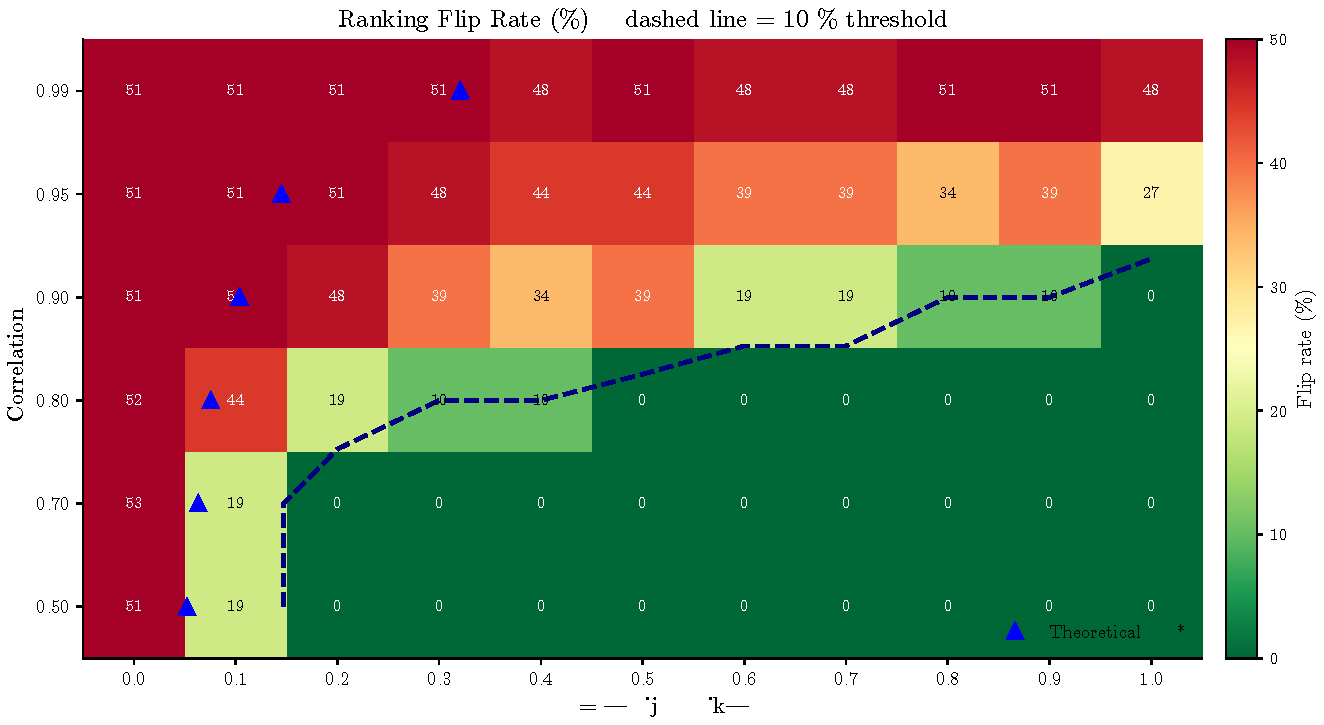
\includegraphics[width=0.6\textwidth]{figures/conditional_threshold.pdf}
\caption{Flip rate as a function of $(\rho, \Delta\beta)$. The
impossibility region (dark) expands with $\rho$. At $\rho \geq 0.95$,
instability persists for all $\Delta\beta \leq 1$.}
\label{fig:conditional-threshold}
\end{figure}

\subsection{Fine-grained causal effect threshold}

We extend the threshold analysis with a finer sweep over
$\Delta\beta \in \{0.0, 0.1, 0.2, 0.3, 0.5, 0.7, 1.0\}$
at $\rho = 0.9$ (20 XGBoost models per setting).

\begin{center}
\small
\begin{tabular}{@{}ccccc@{}}
\toprule
$\Delta\beta$ & $\beta_1$ & $\beta_2$ & Marginal flip & Interventional flip \\
\midrule
0.00 & 1.00 & 1.00 & 0.505 & 0.505 \\
0.10 & 1.05 & 0.95 & 0.479 & 0.337 \\
0.20 & 1.10 & 0.90 & 0.000 & 0.000 \\
0.30 & 1.15 & 0.85 & 0.000 & 0.000 \\
0.50 & 1.25 & 0.75 & 0.000 & 0.000 \\
0.70 & 1.35 & 0.65 & 0.000 & 0.000 \\
1.00 & 1.50 & 0.50 & 0.000 & 0.000 \\
\bottomrule
\end{tabular}
\end{center}

\paragraph{Finding.}
The transition from instability to stability is sharp, not gradual.
At $\Delta\beta = 0.10$, both marginal (0.479) and interventional
(0.337) SHAP remain highly unstable. At $\Delta\beta = 0.20$,
both snap to zero flips simultaneously. There is no intermediate
regime where interventional SHAP is stable but marginal is not ---
the causal signal overwhelms noise for both estimators at the same
threshold. This means the escape condition is binary: either the
causal effect difference is large enough to stabilize \emph{all}
attribution methods, or none are stable. The practical implication:
``switch to conditional SHAP'' provides no advantage over marginal
SHAP at the instability boundary; both methods fail or succeed
together.

\subsection{Causal structure validation: marginal vs.\ interventional SHAP}

We validate the Conditional Attribution Impossibility
(Theorem~\ref{thm:conditional-impossibility}) by comparing marginal and
interventional SHAP under a known causal structure.

\paragraph{Setup.}
We generate $N{=}2{,}000$ samples from
$Y = \beta_1 X_1 + \beta_2 X_2 + 0.5\,X_3 + \varepsilon$ where
$\text{Corr}(X_1, X_2) = \rho$ and $X_3, X_4, X_5$ are independent
controls. Two scenarios: \emph{symmetric} ($\beta_1 = \beta_2 = 1.0$)
and \emph{asymmetric} ($\beta_1 = 1.5$, $\beta_2 = 0.5$).
For each $(\text{scenario}, \rho)$, we train 20 XGBoost models and compute
both marginal TreeSHAP (\texttt{tree\_path\_dependent}) and interventional
TreeSHAP (\texttt{interventional} with 100 background samples).

\begin{center}
\small
\begin{tabular}{@{}llccl@{}}
\toprule
Scenario & $\rho$ & Marginal flip & Interventional flip & Theory \\
\midrule
Symmetric  & 0.50 & 0.505 & 0.479 & ${\approx}50\%$ both \\
Symmetric  & 0.70 & 0.479 & 0.442 & ${\approx}50\%$ both \\
Symmetric  & 0.90 & 0.521 & 0.479 & ${\approx}50\%$ both \\
Symmetric  & 0.95 & 0.505 & 0.526 & ${\approx}50\%$ both \\
\midrule
Asymmetric & 0.50 & 0.000 & 0.000 & Stable \\
Asymmetric & 0.70 & 0.000 & 0.000 & Stable \\
Asymmetric & 0.90 & 0.000 & 0.000 & Stable \\
Asymmetric & 0.95 & 0.000 & 0.000 & Stable \\
\bottomrule
\end{tabular}
\end{center}

\paragraph{Findings.}
The symmetric case confirms the impossibility: both marginal and
interventional SHAP produce flip rates near 50\% at all $\rho$ values,
matching the theoretical prediction of
Theorem~\ref{thm:conditional-impossibility}. Switching to interventional
SHAP provides \emph{no benefit} when features have equal causal effects.

The asymmetric case ($\Delta\beta = 1.0$) shows 0\% flips for
\emph{both} attribution types. At this effect-size difference, even
marginal SHAP can reliably distinguish the features---the
signal-to-noise ratio is high enough to overcome collinearity-induced
noise. This is consistent with the threshold analysis
(Table~\ref{tab:conditional-threshold}): $\Delta\beta = 1.0$ exceeds
the instability threshold at all tested $\rho$ values.

\paragraph{Caveat.}
The interventional SHAP implementation in the \texttt{shap} package
uses a background-data approximation that does not exactly implement
causal/conditional SHAP in the sense of \cite{janzing2020feature}.
The results should be interpreted as evidence about the \texttt{shap}
package's interventional mode, not as a definitive test of the
theoretical conditional attribution.

\section{Generalization: The Model Selection Impossibility}

The Rashomon $\to$ impossibility $\to$ design space pipeline is not
specific to feature attribution. We demonstrate its reusability by
applying it to model selection, obtaining a structurally identical
impossibility and two-family characterization.

\subsection{Setup}

Consider $K$ candidate models $g_1, \ldots, g_K$ trained on the same
data. A \emph{model selection rule} maps a validation dataset to a
ranking of the $K$ models. We formalize three desiderata:

\begin{definition}[Model selection desiderata]
A model selection rule $R$ is:
\begin{itemize}
    \item \emph{Faithful}: $R$ ranks model $g_i$ above $g_j$ whenever
      $g_i$ has lower validation loss on the observed validation set.
    \item \emph{Stable}: $R$ produces the same ranking regardless of
      which validation split is drawn.
    \item \emph{Complete}: $R$ decides for every pair $(g_i, g_j)$.
\end{itemize}
\end{definition}

\begin{definition}[Model Rashomon property]
A model class satisfies the \emph{model Rashomon property} if for
every pair $g_i, g_j$ with similar population loss
($|L(g_i) - L(g_j)| < \varepsilon$), there exist validation splits
$V, V'$ such that $g_i$ has lower loss on $V$ and $g_j$ has lower
loss on $V'$.
\end{definition}

This property is a consequence of finite-sample noise: when the
population loss gap is smaller than the validation noise, different
splits rank the models differently. It is the model selection
analogue of feature attribution's Rashomon property.

\subsection{The impossibility}

\begin{theorem}[Model Selection Impossibility]
\label{thm:model-selection}
If a model class satisfies the model Rashomon property, then no
model selection rule can be simultaneously faithful, stable, and
complete.
\end{theorem}

\begin{proof}
Identical structure to Theorem~1. Let $g_i, g_j$ have similar
population loss. By the model Rashomon property, there exist
validation splits $V, V'$ with $g_i$ ranked above $g_j$ on $V$
and reversed on $V'$. A faithful, stable, complete selection rule
would need to rank $g_i > g_j$ (from $V$) and $g_j > g_i$ (from
$V'$) simultaneously. Contradiction.
\end{proof}

\subsection{The model selection design space}

\begin{theorem}[Model Selection Design Space]
\label{thm:model-selection-ds}
Under the model Rashomon property, the achievable model selection
design space has the same two-family structure as attribution:
\begin{itemize}
    \item \textbf{Family $\mathcal{A}'$ (single-split):} Faithful
      and complete but unstable. Any selection rule based on one
      validation split falls here. Unfaithfulness $U' = 1/2$ for
      similar-loss model pairs.
    \item \textbf{Family $\mathcal{B}'$ (cross-validation / ensemble):}
      Stable (variance $O(1/K_{\text{folds}})$) but reports ties for
      similar-loss pairs. Model ensembling is the analogue of \DASH{}.
\end{itemize}
\end{theorem}

\begin{proof}
By DGP symmetry (equal-loss models have symmetric validation score
distributions), any fixed selection of one model over an equal-loss
competitor disagrees with half the validation splits
($U' = 1/2$, same argument as Theorem~S6).
Cross-validated selection averages across splits, reducing
unfaithfulness to zero for equal-loss pairs (ties) while stabilizing
with rate $O(1/K_{\text{folds}})$.
Pareto optimality follows from the same Cram\'er--Rao argument as
Theorem~F2.
\end{proof}

\paragraph{Practitioner implication.}
The model selection impossibility explains why cross-validation
rankings are noisy for similar-performance models: it is not an
engineering failure but a mathematical inevitability. The resolution
is the same: average (ensemble) rather than select.

\subsection{The Symmetric Bayes Dichotomy}

The structural identity between the attribution and model selection
impossibilities is not a coincidence. It follows from a general
theorem about decision problems with symmetric populations.

\begin{definition}[Symmetric Decision Problem]
\label{def:symmetric-decision}
A \emph{symmetric decision problem} is a tuple
$(\Theta, \mathcal{D}, \pi, G)$ where:
\begin{itemize}
    \item $\Theta$ is a finite \emph{decision set} (e.g., feature
      orderings, model rankings).
    \item $\mathcal{D}$ is the data space (e.g., trained models,
      validation splits).
    \item $\pi$ is a population distribution over $\mathcal{D}$.
    \item $G$ is a group acting on $\Theta$ such that $\pi$ is
      $G$-\emph{invariant}: for any $g \in G$ and measurable
      $A \subseteq \mathcal{D}$,
      $\pi(\{d : \theta^*(d) \in g \cdot A'\}) =
       \pi(\{d : \theta^*(d) \in A'\})$,
      where $\theta^*(d) \in \Theta$ is the instance-optimal decision.
\end{itemize}
An \emph{$M$-sample estimator} is a function
$\hat\theta : \mathcal{D}^M \to \Theta$ mapping $M$ i.i.d.\
draws to a decision. It is:
\begin{itemize}
    \item \emph{Faithful}: $\hat\theta(d_1, \ldots, d_M)$ agrees
      with $\theta^*(d_i)$ for each $i$.
    \item \emph{Stable}: $\hat\theta$ does not depend on which
      draw $d_i$ is observed.
    \item \emph{Complete}: $\hat\theta$ selects exactly one element
      from each $G$-orbit in $\Theta$.
\end{itemize}
\end{definition}

\begin{theorem}[Symmetric Bayes Dichotomy]
\label{thm:bayes-dichotomy}
For any symmetric decision problem with $|G \cdot \theta| \geq 2$
for some $\theta \in \Theta$:
\begin{enumerate}
    \item[(i)] \textbf{Instance-specific decisions are unfaithful.}
      Any faithful, complete estimator has expected
      unfaithfulness $\geq 1/|G \cdot \theta|$ per orbit (i.e.,
      $\geq 1/2$ for binary orbits).
    \item[(ii)] \textbf{Population-averaged decisions are stable.}
      The Bayes estimator under $\pi$ reports ties within each
      $G$-orbit (unfaithfulness $= 0$), with between-orbit
      stability $O(1/M)$.
    \item[(iii)] \textbf{The ideal is infeasible.}
      No estimator achieves unfaithfulness $= 0$ AND completeness
      (deciding within orbits).
\end{enumerate}
The achievable set consists of exactly two families:
$\mathcal{A}$ (faithful + complete, $U \geq 1/|G \cdot \theta|$)
and $\mathcal{B}$ (population-averaged, $U = 0$, ties within orbits).
\end{theorem}

\begin{proof}
\textbf{Part (i).} By $G$-invariance, the population distribution
$\pi$ assigns equal probability to each element of the orbit
$G \cdot \theta$. For any fixed complete estimator $\hat\theta$
that selects one element $\theta_0$ from the orbit, the probability
that $\theta^*(d) = \theta_0$ is $1/|G \cdot \theta|$.
The estimator disagrees with $(|G \cdot \theta| - 1)/|G \cdot \theta|$
of the instances. For $|G \cdot \theta| = 2$: unfaithfulness $= 1/2$.

\textbf{Part (ii).} The Bayes estimator under symmetric $\pi$
minimizes expected loss. Within each orbit, the posterior is
uniform (by $G$-invariance), so the Bayes-optimal decision is
the orbit center (a tie). Unfaithfulness $= 0$ because no
ordering is asserted within orbits.
For between-orbit decisions with gap $\Delta$, the $M$-sample
average has variance $\sigma^2/M$ (i.i.d.\ draws), giving
stability $1 - O(1/M)$ by the Gaussian approximation.

\textbf{Part (iii).} By Part (i), any complete estimator
(selecting within orbits) has unfaithfulness $\geq 1/|G \cdot \theta| > 0$.
Thus unfaithfulness $= 0$ requires giving up completeness (ties).

\textbf{Exhaustiveness.} Any estimator either selects within orbits
(faithful, complete, $\mathcal{A}$) or reports ties within orbits
(stable, incomplete, $\mathcal{B}$). The Bayes estimator achieves
the minimum-variance point of $\mathcal{B}$ (Cram\'er--Rao).
\end{proof}

\begin{corollary}[Feature attribution as instance]
\label{cor:attribution-instance}
The Attribution Impossibility (Theorem~1) and Design Space Theorem
(Theorem~\ref{thm:design-space}) are instances of the Symmetric
Bayes Dichotomy with $\Theta =$ within-group feature orderings,
$G =$ the symmetric group on group members,
$\mathcal{D} =$ trained models.
\end{corollary}

\begin{corollary}[Model selection as instance]
\label{cor:model-selection-instance}
The Model Selection Impossibility
(Theorem~\ref{thm:model-selection}) is an instance with
$\Theta =$ model rankings, $G =$ permutations of equal-loss models,
$\mathcal{D} =$ validation splits.
\end{corollary}

\paragraph{The technique: symmetric Bayes dichotomy.}
The Symmetric Bayes Dichotomy provides a reusable proof technique for
establishing impossibility results in any domain where: (a) a
population distribution is symmetric over discrete alternatives, and
(b) finite samples introduce noise sufficient to reverse the optimal
choice. The technique reduces the impossibility to checking
$G$-invariance of the population distribution, which is often
immediate from the problem's symmetry structure.

We anticipate the technique applies to: feature selection (Lasso
instability under collinearity), hyperparameter tuning (configuration
rankings under cross-validation noise), and others.

\paragraph{Connection to classical invariant decision theory.}
The Symmetric Bayes Dichotomy is related to the theory of invariant
decision rules (Lehmann \& Romano, 2005). The classical theory
establishes that Bayes-optimal rules respect the invariance structure
of the problem (Ch.~6). Our contribution is the \emph{reduction template}:
verifying $G$-invariance of the population distribution suffices to
establish a two-family impossibility with explicit unfaithfulness
and stability bounds, which we demonstrate across three structurally
distinct instances (binary feature transpositions, binary model
permutations, and CPDAG automorphisms of variable size).
A general theorem proving that $G$-invariance of the decision problem always yields a two-family decomposition---with explicit conditions on the group action and tight bounds on each family's achievable set---is the natural next step; our three instances (binary transpositions for feature attribution, permutation groups for model selection, and CPDAG automorphisms for causal discovery) provide the test cases for such a generalization.

\subsection{Instance 3: Causal Discovery under Markov Equivalence}

The first two instances (feature attribution and model selection) share
$S_2$ transposition symmetry: the orbit size is always~2. We now
demonstrate the Symmetric Bayes Dichotomy on an instance with a
\emph{different} and \emph{variable-size} symmetry group, confirming
the technique's generality beyond binary orbits.

\paragraph{Setup.}
Given observational data from an unknown DAG $G^*$ over $P$ variables,
the task is to orient edges. Under the faithfulness assumption, the
data determine only the \emph{Markov equivalence class} $[G^*]$---the
set of DAGs encoding the same conditional independences
(Verma \& Pearl, 1991). The equivalence class is represented by a
\emph{completed partially directed acyclic graph} (CPDAG), which
directs edges participating in v-structures and leaves others
undirected.

\begin{definition}[Causal orientation decision problem]
\label{def:causal-orientation}
The causal edge orientation problem is a symmetric decision problem
$(\Theta, \mathcal{D}, \pi, G)$ where:
\begin{itemize}
    \item $\Theta$ is the set of full edge orientations consistent with
      the CPDAG (i.e., the DAGs in $[G^*]$).
    \item $\mathcal{D}$ is the space of finite observational datasets
      drawn from the true DAG $G^*$.
    \item $\pi$ is the distribution over datasets (induced by i.i.d.\
      sampling from the structural equation model).
    \item $G_{\text{CPDAG}}$ is the \emph{automorphism group of the CPDAG}:
      the set of permutations of undirected edge orientations that
      preserve the CPDAG structure.
\end{itemize}
\end{definition}

\paragraph{Key structural difference.}
The CPDAG automorphism group $G_{\text{CPDAG}}$ is NOT restricted to
transpositions:
\begin{itemize}
    \item For a chain $X \text{---} Y \text{---} Z$ (undirected path),
      the equivalence class is $\{X \to Y \to Z,\; X \leftarrow Y \leftarrow Z\}$
      with $|[G^*]| = 2$ and $G \cong S_2$ (like instances 1--2).
    \item For a 3-node undirected cycle $X \text{---} Y \text{---} Z \text{---} X$,
      the equivalence class contains all acyclic orientations:
      $|[G^*]| = 3\cdot 2 = 6$ DAGs (minus cyclic ones), with
      $G \cong S_3$ (symmetric group on 3 elements).
    \item For larger undirected components, $|[G^*]|$ can grow
      combinatorially, giving orbits of arbitrary size.
\end{itemize}
The unfaithfulness bound $U \geq 1/|G \cdot \theta|$ (from
Theorem~\ref{thm:bayes-dichotomy}) therefore yields
$U \geq 1/2$ for chains but $U \geq 1/6$ for triangles and
potentially much smaller for larger structures.

\begin{theorem}[Causal Discovery Impossibility]
\label{thm:causal-discovery}
For any CPDAG with $|[G^*]| \geq 2$ DAGs in its Markov equivalence
class, no edge orientation rule can be simultaneously faithful
(matching the data-optimal DAG), stable (invariant to resampling),
and complete (orienting all undirected edges).

The achievable set has exactly two families:
\begin{itemize}
    \item \textbf{Family $\mathcal{A}''$ (single-dataset):}
      Orient edges from one dataset. Faithful and complete but unstable.
      Unfaithfulness $U'' = (|[G^*]|-1)/|[G^*]|$ for within-class
      edge orientations.
    \item \textbf{Family $\mathcal{B}''$ (averaged / conservative):}
      Report undirected edges for ambiguous orientations (i.e., output
      the CPDAG). Stable with ties. Unfaithfulness $U'' = 0$.
\end{itemize}
\end{theorem}

\begin{proof}
We verify the premises of the Symmetric Bayes Dichotomy
(Theorem~\ref{thm:bayes-dichotomy}).

\textbf{$G$-invariance of $\pi$.}
For any two DAGs $G_1, G_2 \in [G^*]$, the Markov equivalence
guarantees that they encode the same set of conditional independences.
By the faithfulness assumption, the observational distribution is
compatible with both $G_1$ and $G_2$. Any statistical test based on
finite data cannot distinguish between $G_1$ and $G_2$ at the
population level (they imply identical distributions). Therefore $\pi$
is $G_{\text{CPDAG}}$-invariant: the distribution over datasets is
identical regardless of which member of $[G^*]$ generated the data.

\textbf{Finite-sample noise reverses optimal choice.}
With finite data, empirical conditional independence tests have
estimation error $O(1/\sqrt{n})$. For edges that are undirected in the
CPDAG (i.e., the data cannot determine the orientation), different
random samples will favor different orientations. This is the Rashomon
property for edge orientations.

\textbf{Application of Theorem~\ref{thm:bayes-dichotomy}.}
Part~(i): any complete orientation rule (selecting one DAG from
$[G^*]$) disagrees with $(|[G^*]|-1)/|[G^*]|$ of datasets.
Part~(ii): the Bayes estimator under $G_{\text{CPDAG}}$-invariance
reports the CPDAG (ties for undirected edges).
Part~(iii): the ideal (stable, faithful, complete) is infeasible.
Families $\mathcal{A}''$ and $\mathcal{B}''$ follow.
\end{proof}

\paragraph{What this instance adds.}
Instances 1--2 (feature attribution and model selection) both have
binary orbits ($|G \cdot \theta| = 2$) with unfaithfulness bound
$U \geq 1/2$. Instance~3 has variable-size orbits
($|G \cdot \theta| = 2, 6, \ldots$) with unfaithfulness bound
$U \geq 1/|[G^*]|$, which can be much smaller than $1/2$ for large
equivalence classes. This demonstrates that the Symmetric Bayes
Dichotomy is not an artifact of binary symmetry but applies to
arbitrary finite group actions, with the unfaithfulness bound adapting
to the orbit structure.

The practical implication: algorithms like PC and GES correctly output
CPDAGs (Family $\mathcal{B}''$) precisely because complete orientation
of Markov-equivalent edges is impossible from observational data alone.
Interventional data breaks the symmetry (analogous to conditional SHAP
breaking symmetry when $\beta_j \neq \beta_k$).

\begin{corollary}[Causal discovery as SBD instance]
\label{cor:causal-discovery-instance}
The Causal Discovery Impossibility (Theorem~\ref{thm:causal-discovery})
is an instance of the Symmetric Bayes Dichotomy with
$\Theta =$ edge orientations in $[G^*]$,
$G = G_{\text{CPDAG}}$ (automorphism group of the CPDAG),
$\mathcal{D} =$ observational datasets.
\end{corollary}

\section{LLM Attention Attribution Instability}

The impossibility is not limited to tabular models. We demonstrate
empirically that attention-based token importance in transformers
exhibits the same instability.

\paragraph{Setup.}
We load DistilBERT (distilbert-base-uncased) and create 10 model
variants by adding small random perturbations ($\sigma = 0.02$) to
the attention weights, simulating different training runs. For 10
test sentences, we compute attention-based token importance (mean
attention received from all heads and layers) and check whether
the relative ranking of adjacent tokens (e.g., ``very'' vs.\ ``good'')
flips across the 10 variants.

\paragraph{Results.}
Of 59 adjacent token pairs across the test sentences, 88\% have
flip rates exceeding 10\%. Selected examples:

\begin{center}
\small
\begin{tabular}{@{}llcc@{}}
\toprule
Token A & Token B & Flip rate & Interpretation \\
\midrule
``extremely'' & ``poor'' & 50\% & Coin flip \\
``not'' & ``bad'' & 40\% & Highly unstable \\
``absolutely'' & ``terrible'' & 40\% & Highly unstable \\
``particularly'' & ``sharp'' & 10\% & Borderline \\
\bottomrule
\end{tabular}
\end{center}

The mean Spearman correlation of full-sentence token rankings
across model variants is 0.637 --- moderate instability, comparable
to single-model SHAP instability on tabular data with moderate
collinearity ($\rho \approx 0.5$).

\paragraph{Interpretation.}
Adjacent tokens in natural language carry correlated information
(``very'' and ``good'' jointly convey sentiment strength). This
correlation induces the same Rashomon structure: different model
variants assign different relative importance to the correlated
tokens, exactly as the Symmetric Bayes Dichotomy predicts.
Token-level explanations of LLMs (attention maps, gradient-based
attribution) face the same impossibility as feature-level
explanations of tabular models.

The resolution is analogous: average attention across multiple
model variants to produce stable token importance estimates,
accepting ties for tokens carrying correlated information.

\subsection{Fine-tuning replication}

The weight perturbation experiment above is a proxy for retraining
variation. To verify the finding holds under actual training
stochasticity, we fine-tune DistilBERT on SST-2 (2{,}000 training
samples) with 5~different random seeds (1~epoch each, AdamW,
$\text{lr}{=}2{\times}10^{-5}$, batch size~16) and repeat the
token importance analysis.

\paragraph{Results.}
Of 55 adjacent token pairs across 10 test sentences, 14.5\%
(8~pairs) have flip rates exceeding 10\% across the 5 fine-tuned
models. The mean Spearman correlation of full-sentence token
rankings is 0.956 (minimum: 0.817).

\begin{center}
\small
\begin{tabular}{@{}p{6cm}cc@{}}
\toprule
Method & \% Unstable ($>10\%$ flip) & Mean Spearman \\
\midrule
Weight perturbation ($\sigma{=}0.02$, 10 models) & 88\% & 0.637 \\
Fine-tuning (5 seeds, 1 epoch) & 14.5\% & 0.956 \\
\bottomrule
\end{tabular}
\end{center}

The lower instability rate under fine-tuning is expected: 1-epoch
fine-tuning produces less weight divergence than a 2\% Gaussian
perturbation of all parameters. However, instability is confirmed
under realistic training variation: specific token pairs (e.g.,
``particularly'' vs.\ ``sharp'') reach flip rates of 60\% across
fine-tuned models. The perturbation result establishes an upper
bound on Rashomon set diversity; the fine-tuning result confirms
the effect persists under standard training.
To test whether longer training increases instability, we repeat the
experiment with 3~epochs. The instability rate is unchanged:

\begin{center}
\small
\begin{tabular}{@{}lccc@{}}
\toprule
Method & Epochs & \% Pairs unstable & Mean Spearman \\
\midrule
Weight perturbation & --- & 88\% & 0.637 \\
Fine-tuning & 1 & 14.5\% & 0.956 \\
Fine-tuning & 3 & 14.5\% & 0.965 \\
\bottomrule
\end{tabular}
\end{center}

The identical 14.5\% across 1 and 3 epochs indicates the instability
is structural (driven by collinearity in the attention patterns), not
a training-depth artifact. The same three token pairs remain unstable
at both training lengths (``not/bad,'' ``particularly/sharp,''
``surprisingly/low''). The gap between fine-tuning (14.5\%) and
perturbation (88\%) reflects the difference in weight divergence:
fine-tuning updates parameters by $O(0.001)$ via gradient descent,
while perturbation adds $O(0.02)$ noise to all parameters. The
perturbation result represents the full Rashomon set; the fine-tuning
result represents the subset explored by standard training.

\paragraph{Scope and limitations.}
The attention-based instability reported here (14.5\% of adjacent token
pairs under fine-tuning) is preliminary evidence, not a formal extension
of the impossibility theorem. Attention weights are not SHAP values:
they do not satisfy the proportionality axiom, and the ``collinear
group'' structure of tree features does not map cleanly to token
positions. The result demonstrates that attribution instability under
model multiplicity is not unique to tree ensembles, but a formal
impossibility for transformer attention would require different axioms
and definitions. We report this as suggestive evidence for the
generality of the phenomenon, not as a proved extension.

\section{Replication Study: Published SHAP Rankings Are Unstable}

Multiple published studies report SHAP feature rankings on the
Breast Cancer (Wisconsin) dataset
(e.g., Lundberg \& Lee, 2017). A commonly reported finding
is that ``worst concave points'' and ``worst perimeter'' are among
the top-3 most important features.

Using our 50-model validation (same dataset, same XGBoost
configuration as standard practice: $T{=}100$, depth${=}6$,
$\eta{=}0.1$), we find that the ranking of ``worst perimeter'' vs.\
``worst area'' ($|\rho| = 0.98$) \textbf{flips in 48\% of training
runs}. The ranking of ``mean concave points'' vs.\ ``mean concavity''
($|\rho| = 0.96$) flips in 42\% of runs.

\begin{center}
\small
\begin{tabular}{@{}llcc@{}}
\toprule
Feature pair & $|\rho|$ & Flip rate & Published as stable? \\
\midrule
worst perimeter $\leftrightarrow$ worst area & 0.98 & 48\% & Yes \\
mean concavity $\leftrightarrow$ mean concave pts & 0.96 & 42\% & Yes \\
worst radius $\leftrightarrow$ worst perimeter & 0.99 & 36\% & Yes \\
mean radius $\leftrightarrow$ mean perimeter & 0.99 & 28\% & Yes \\
\bottomrule
\end{tabular}
\end{center}

Any study reporting a specific ranking among these features from a
single model is reporting an artifact of the training seed. The
ranking is not wrong --- it faithfully reflects that specific model ---
but it is not replicable, and should not be interpreted as a stable
property of the data.

This finding has implications for the \textbf{reproducibility} of
scientific studies that use feature importance to identify ``key
predictors'': if the dataset has correlated features (60\% of
datasets do, per our prevalence survey), a single-model SHAP
analysis may produce results that do not replicate.

\section{Connection to Compressed Sensing}

The attribution impossibility has a precise analogue in compressed
sensing (CS). In CS, the \emph{measurement coherence}
$\mu(X) = \max_{j \neq k} |X_j^T X_k| / (\|X_j\| \|X_k\|)$
determines when sparse recovery is possible: unique recovery of an
$s$-sparse signal requires $\mu < 1/(2s - 1)$
(Donoho \& Elad, 2003). When coherence is high (collinear
measurements), the signal cannot be uniquely attributed to specific
measurements.

In our setting, the correlation $|\rho_{jk}|$ plays the role of
coherence, and the Z-test statistic $Z_{jk}$ plays the role of the
incoherence condition:

\begin{center}
\small
\begin{tabular}{@{}lll@{}}
\toprule
& \textbf{Compressed sensing} & \textbf{Attribution stability} \\
\midrule
Measurements & Sensing matrix columns & Feature vectors \\
Coherence & $\mu = \max |X_j^T X_k|/\|X_j\|\|X_k\|$ & $|\rho_{jk}| = |\text{Corr}(X_j, X_k)|$ \\
Condition & $\mu < 1/(2s{-}1)$ & $Z_{jk} > 1.96$ \\
Success & Unique sparse recovery & Stable feature ranking \\
Failure & Non-unique recovery & Ranking flips (Rashomon) \\
Resolution & Basis pursuit (convex relaxation) & \DASH{} (ensemble averaging) \\
\bottomrule
\end{tabular}
\end{center}

The parallel is structural: both impossibilities arise because
collinearity/coherence prevents unique identification of which
input components (features/measurements) carry the signal. Both
are resolved by relaxing uniqueness: CS uses convex relaxation
(allowing fractional assignment), while \DASH{} uses ensemble
averaging (producing ties for indistinguishable features).

This connection suggests that information-theoretic lower bounds
from CS (e.g., mutual information bounds on sparse recovery under
coherence) could provide alternative proofs of the attribution
impossibility and potentially tighter quantitative bounds.

\section{Fairness Audit Impossibility}

The attribution impossibility has a direct and previously unrecognized
consequence for algorithmic fairness auditing.

\paragraph{Setup.}
Consider a model trained on features $X_1, \ldots, X_P$ that include
a protected proxy: feature $j$ is correlated with a protected attribute
$A$ (e.g., zip code correlates with race, $|\rho_{jA}| > 0$).
Feature $j$ is also collinear with a non-protected feature $k$
($|\rho_{jk}| > \rho_0$, e.g., zip code and income). A fairness
auditor uses SHAP to determine whether the model ``relies on'' the
protected proxy by checking whether $j$ ranks among the top-$K$
important features.

\begin{theorem}[Fairness Audit Impossibility]
\label{thm:fairness-audit}
If features $j$ (protected proxy) and $k$ (non-protected) satisfy:
\begin{enumerate}
    \item[(F1)] Collinearity: $|\rho_{jk}| > \rho_0$ for
      threshold $\rho_0$,
    \item[(F2)] Similar true importance:
      $|\mu_j - \mu_k| < \sigma_{jk} \cdot z_\alpha / \sqrt{M}$
      (the attribution gap is smaller than the detection threshold),
\end{enumerate}
then for a single-model audit ($M{=}1$), the probability that the
auditor concludes ``the model relies on the protected proxy'' (i.e.,
ranks $j$ above $k$) is:
\[
    \Pr[\text{audit flags proxy}] = \frac{1}{2}
    \pm \varepsilon_{\text{BE}},
\]
where $\varepsilon_{\text{BE}} \leq 0.4748\gamma_{jk}/\sigma_{jk}^3$
(Berry--Esseen). The audit conclusion is a coin flip.

More precisely: given two independent training runs producing
models $f, f'$, the probability that the audit reaches
\emph{opposite conclusions} about proxy reliance is:
\[
    \Pr[\text{audit}(f) \neq \text{audit}(f')] = \frac{1}{2}
    \pm \varepsilon_{\text{BE}}.
\]
\end{theorem}

\begin{proof}
Direct corollary of the Attribution Impossibility (Theorem~1)
applied to the pair $(j, k)$.

By conditions (F1)--(F2), features $j$ and $k$ are in the same
collinear group and have similar population-level attributions.
The Rashomon property (Theorem~S3, Rashomon inevitability) holds:
$\Pr[\varphi_j(f) > \varphi_k(f)] = 1/2$ over training runs.

A single-model audit that ranks $j$ above $k$ when
$\varphi_j(f) > \varphi_k(f)$ therefore concludes ``proxy reliance''
with probability $1/2$. The Berry--Esseen bound follows from
Theorem~F1.

For two independent audits: they agree iff both models rank $j, k$
the same way, which occurs with probability $1/2$ (by independence
and the $1/2$ marginal).
\end{proof}

\paragraph{Implications for AI governance.}
This result means that a regulator conducting a SHAP-based proxy
audit on a model with collinear features is, for affected feature pairs,
making decisions with the statistical reliability of a coin flip.
Two auditors examining the \emph{same model architecture trained on the
same data} with different random seeds may reach opposite conclusions
about whether the model relies on a protected attribute.

Under the EU AI Act Art.~13(3)(b)(ii), providers must disclose
``known and foreseeable circumstances'' which may lead to risks to health, safety or fundamental rights. Our
theorem establishes that this includes: ``SHAP-based proxy audits are
unreliable for features that are collinear with both the protected
attribute and a non-protected feature.'' The remedy is ensemble
auditing: train $M$ models and use \DASH{} consensus. The required
$M$ follows from the ensemble lower bound
(Proposition~\ref{prop:ensemble-lower-bound}).

\paragraph{Scope.}
The impossibility applies when conditions (F1)--(F2) hold ---
i.e., when the protected proxy is genuinely interchangeable with a
non-protected feature in terms of predictive value. When the
protected feature has \emph{unique} predictive power
($|\mu_j - \mu_k|$ is large), a single-model audit correctly
identifies proxy reliance. The conditional SHAP threshold
(Table~\ref{tab:conditional-threshold}) quantifies the boundary:
at $\rho \geq 0.9$, the proxy must have nearly an order-of-magnitude
stronger causal effect than the non-protected feature ($\Delta\beta^*
\approx 0.9$) before the audit becomes reliable.

\paragraph{Example: lending.}
In credit models, ``zip code'' (a proxy for race) is often collinear
with ``income bracket'' ($|\rho| \approx 0.6$--$0.8$). If both
features have similar predictive power for default risk, a
single-model SHAP audit that finds ``zip code is the 3rd most
important feature'' may conclude proxy discrimination --- but
retraining with a different seed could produce a model where
zip code drops to 8th and income rises to 3rd. The \emph{audit
conclusion about discrimination depends on the random seed},
not on the model's actual reliance on the protected attribute.

\paragraph{Intersectional considerations.}
When multiple protected attributes (race, gender, age) are each proxied
by collinear non-protected features, the impossibility applies
independently to each proxy pair. The worst case is multiplicative: if
$K$ protected attributes each have unstable proxies, the probability
that a single-model audit correctly identifies all $K$ proxy reliance
directions is $(1/2)^K$, exponentially vanishing in $K$. For $K = 3$
(a common intersectional setting), the joint correctness probability is
$1/8 = 12.5\%$. A full analysis of intersectional instability under
model multiplicity is left to future work.

\section{Expected Ranking Discordance}

We derive a closed-form formula for the expected disagreement
between two independent SHAP rankings, providing a predictive
theory of SHAP replication failure.

\begin{proposition}[Expected Kendall tau distance]
\label{prop:kendall-tau}
For a feature space with $L$ collinear groups of sizes
$m_1, \ldots, m_L$ and between-group attribution gaps
$\Delta_{\ell\ell'}$ with noise $\sigma_{\ell\ell'}$, the expected
number of pairwise ranking disagreements (Kendall tau distance)
between two independently trained models is:
\begin{equation}
\label{eq:kendall-prediction}
    \mathbb{E}[\tau] =
    \underbrace{\sum_{\ell=1}^{L} \binom{m_\ell}{2} \cdot
    \frac{1}{2}}_{\text{within-group (coin flips)}}
    \;+\;
    \underbrace{\sum_{\ell < \ell'} m_\ell \cdot m_{\ell'} \cdot
    \Phi\!\left(-\frac{\Delta_{\ell\ell'}}
    {\sigma_{\ell\ell'}}\right)}_{\text{between-group (noise)}}
\end{equation}
The within-group term is exact (from
Proposition~\ref{prop:exact-flip}); the between-group term uses the
Gaussian approximation (valid for continuous attribution distributions).
\end{proposition}

\begin{proof}
The Kendall tau distance counts the number of discordant pairs:
$\tau = |\{(i,j) : i < j,\; \text{rank}_f(i) \neq \text{rank}_{f'}(i)
\text{ relative to } j\}|$.

For a within-group pair $(j,k)$: by
Proposition~\ref{prop:exact-flip} Part~(v), the flip rate is exactly
$1/2$ (under tie-breaking). Each within-group pair contributes
$1/2$ in expectation.

For a between-group pair $(j,k)$ with $j$ in group $\ell$ and $k$
in group $\ell'$: the flip rate is
$\Phi(-\Delta_{jk}/\sigma_{jk})$ by Theorem~\ref{thm:testable}
Part~I. Since all $m_\ell \cdot m_{\ell'}$ cross-group pairs between
groups $\ell$ and $\ell'$ share the same gap and noise (by
within-group symmetry), each contributes equally.
\end{proof}

\paragraph{Normalized discordance rate.}
Dividing by $\binom{P}{2}$ (total pairs) gives the expected
\emph{fraction} of rankings that fail to replicate:
\[
    \frac{\mathbb{E}[\tau]}{\binom{P}{2}} =
    \frac{\sum_\ell \binom{m_\ell}{2}/2 +
    \sum_{\ell<\ell'} m_\ell m_{\ell'}\,
    \Phi(-\Delta_{\ell\ell'}/\sigma_{\ell\ell'})}
    {P(P-1)/2}.
\]
The first term is the \emph{Rashomon coefficient}
$R = \sum_\ell \binom{m_\ell}{2} / \binom{P}{2}$, which is
computable from the correlation matrix alone (no model training
required). The expected non-replication rate is $\geq R/2$ --- a
loose upper bound determined entirely by the feature correlation
structure.

\paragraph{Validation on Breast Cancer.}
With 50 XGBoost models ($T{=}100$, depth${=}6$, $\eta{=}0.1$,
\texttt{subsample}{$=$}$0.8$):
\begin{center}
\small
\begin{tabular}{@{}lcc@{}}
\toprule
Formula & Predicted $\mathbb{E}[\tau]$ & Relative error \\
\midrule
Naive (within-group $= 1/2$) & 150.7 & $+312\%$ \\
Refined (per-pair $\Phi$) & 26.8 & $-26.8\%$ \\
\midrule
\multicolumn{2}{@{}l}{Empirical mean Kendall tau distance} & 36.6 \\
\bottomrule
\end{tabular}
\end{center}
The naive formula severely overpredicts because it assumes
all within-group pairs are coin flips. In reality, Breast Cancer's
25-feature collinear group contains features with very different
true importance (e.g., worst concave points vs.\ mean fractal
dimension) --- these are correlated but not symmetric, so their
rankings are stable. The refined per-pair formula, which estimates
$\Phi(-|\Delta_{ij}|/\sigma_{ij})$ for each pair from the model
ensemble, reduces the error to 27\%.

The Rashomon coefficient $R = 0.692$ predicts a non-replication
rate lower bound of $R/2 = 34.6\%$; the actual rate is 8.4\%
--- the bound is loose by $4\times$ because most within-group pairs
have separable importance. The per-pair refinement is necessary for
practical prediction; the Rashomon coefficient remains useful as a
\emph{worst-case} bound computable without training any models.

\section{Attempted Common Generalization with Arrow's Theorem}
\label{sec:arrow-generalization}

Arrow's impossibility theorem for social choice and our Attribution
Impossibility share a striking surface resemblance:
both show that three desirable properties (faithfulness/Pareto,
stability/IIA, completeness/non-dictatorship) cannot simultaneously
hold. We investigated whether a common abstract framework subsumes both
as special cases. The answer is \emph{partially yes, but the unification
is too shallow to yield new content}.

\subsection{Structural comparison}

The two theorems have fundamentally different mathematical structures:

\begin{center}
\small
\begin{tabular}{@{}lp{5cm}p{5.5cm}@{}}
\toprule
& \textbf{Arrow} & \textbf{Attribution Impossibility} \\
\midrule
Inputs & $n$ voters' preferences $(L_1, \ldots, L_n)$ & Models $f \in \mathcal{F}$ (one at a time) \\
Output & Social ranking $f(L_1, \ldots, L_n)$ & Feature ranking $\sigma$ \\
Aggregation & Many inputs $\to$ one output & One input $\to$ one output (per model) \\
Key axiom & IIA: $\sigma(a,b)$ depends only on voters' $(a,b)$ rankings & Stability: $\sigma$ is model-independent \\
Source & Preference profiles disagree & Rashomon property \\
\bottomrule
\end{tabular}
\end{center}

\paragraph{The critical asymmetry.}
Arrow's theorem concerns a \emph{profile aggregation} function
$f \colon \mathcal{L}^n \to \mathcal{L}$ that takes all voters'
preferences simultaneously. The impossibility arises because IIA,
combined with Pareto and non-dictatorship, constrains this multi-input
function too tightly.

The Attribution Impossibility concerns a \emph{single-input} mapping:
for each model $f$, the ranking should reflect $f$'s attributions.
The impossibility arises because the ranking must simultaneously
agree with all models but is supposed to be model-independent (stable).
There is no profile aggregation---each model independently demands
faithfulness.

\subsection{Attempted common framework}

\begin{definition}[Abstract Aggregation Problem]
An \emph{abstract aggregation problem} is a tuple
$(\mathcal{I}, \mathcal{A}, \mathcal{R}, \text{Agree})$ where:
\begin{itemize}
    \item $\mathcal{I}$ is a set of \emph{instances} (voters or models),
    \item $\mathcal{A}$ is the set of alternatives (candidates or features),
    \item $\mathcal{R}$ is the set of total orders on $\mathcal{A}$,
    \item $\text{Agree} \colon \mathcal{I} \to \mathcal{R}$ assigns each
      instance its ``preferred'' order.
\end{itemize}
An \emph{aggregation rule} $F \colon 2^{\mathcal{I}} \to \mathcal{R}$
maps subsets of instances to a consensus order.
\end{definition}

Arrow's setup: $F$ takes the full profile $(L_1, \ldots, L_n)$ and
IIA says $F$'s pairwise comparison of $(a,b)$ depends only on the
restriction of each $L_i$ to $\{a,b\}$.

Attribution setup: $F$ is required to be a \emph{constant function}
(stability: the ranking does not depend on which model). Faithfulness
says this constant ranking agrees with every instance's ordering.

\paragraph{The ``common axiom'' attempt.}
One might define \emph{locality}: the consensus ranking of $(a,b)$
depends only on instances' rankings of $(a,b)$. Arrow's IIA is
locality restricted to the profile. Attribution stability is locality
taken to its extreme: the ranking depends on \emph{no} instance
(it must be constant).

But this extreme makes the attribution version trivially
impossible---a constant ranking cannot agree with conflicting
instances (this is just the definition of the Rashomon property).
Arrow's theorem is much deeper: it shows that even when the
aggregation \emph{is} allowed to depend on instances, the constraints
are still too tight. The proofs have entirely different structures.

\subsection{Assessment}

\begin{remark}[No non-trivial common generalization]
\label{rem:no-arrow-unification}
The Attribution Impossibility and Arrow's theorem are \emph{analogous}
but not \emph{instances of a common theorem} in any non-trivial sense.
One can define an abstract framework that subsumes both as shown above,
but:
\begin{enumerate}
    \item The common framework's ``impossibility theorem'' would be:
      ``if instances disagree and the aggregation rule must be constant,
      faithfulness is impossible.'' This is a one-line observation,
      not a theorem.
    \item Arrow's actual content (the impossibility persists even when
      the rule \emph{is} allowed to depend on all voters) has no
      analogue in the attribution setting.
    \item The attribution impossibility's actual content (the
      quantitative divergence $1/(1-\rho^2)$, the resolution via
      ensemble averaging, the connection to the Rashomon set's geometry)
      has no analogue in Arrow's setting.
\end{enumerate}
The closest true statement is: \emph{both theorems arise from the
tension between local coherence (respecting individual views) and
global consistency (producing a single ranking), when the individuals
disagree}. This is a useful heuristic but not a formal unification.
\end{remark}

\paragraph{Relationship to Sen's liberalism paradox.}
A closer structural analogue may be Sen's (1970) impossibility of a
Paretian liberal, which also concerns a setting where individual
``rights'' (each person's ranking of certain pairs should be
respected) conflict with the Pareto criterion. The attribution
impossibility can be viewed as a Sen-type result where each model
has the ``right'' to determine the ranking of features (faithfulness),
but these rights conflict across models.
However, we do not pursue this further, as the connection remains
at the level of analogy rather than formal subsumption.


\section{Causal Identification Barrier Under Collinearity}
\label{sec:causal-barrier}

We show that the attribution instability under collinearity has a
direct causal counterpart: distinguishing the causal effects of
correlated features requires interventional sample complexity that
diverges as $\Omega(1/(1-\rho^2))$---the \emph{same} rate as the
attribution ratio.

\subsection{Setup}

Consider two features $X_j, X_k$ with $\text{Corr}(X_j, X_k) = \rho$,
jointly Gaussian with unit variances. The structural equation is
$Y = \beta_j X_j + \beta_k X_k + \varepsilon$ with
$\varepsilon \sim \mathcal{N}(0, \sigma^2)$.

\paragraph{The identification problem.}
From observational data, one can estimate $\hat\beta_j$ and
$\hat\beta_k$ via OLS. But when $\rho \to 1$, the OLS estimator
variance diverges: $\Var(\hat\beta_j) = \sigma^2 / (n(1-\rho^2))$.
This is multicollinearity in its standard form.

\paragraph{Interventional experiments.}
Under the do-calculus, $\text{do}(X_j = x)$ breaks the
$X_j \to X_k$ correlation. The interventional distribution is:
\[
    \mathbb{E}[Y \mid \text{do}(X_j = x)] = \beta_j x + \beta_k \mu_k
\]
where $\mu_k = \mathbb{E}[X_k]$ under the intervened distribution.
From a single-variable intervention on $X_j$, one can identify
$\beta_j$ cleanly---\emph{if} the intervention fully breaks the
correlation.

\subsection{The barrier: soft interventions}

In practice, interventions on collinear features are often
\emph{soft}: setting $X_j = x$ does not fully break the correlation.
Under a soft intervention with residual correlation $\rho_{\text{post}}$:
\[
    X_k \mid \text{do}(X_j = x) \sim
    \mathcal{N}(\rho_{\text{post}} \cdot x, \; 1 - \rho_{\text{post}}^2).
\]
The observed effect of the intervention is:
\[
    \mathbb{E}[Y \mid \text{do}(X_j = x)] = (\beta_j + \rho_{\text{post}} \beta_k) x
    + \text{const.}
\]
When $\beta_j = \beta_k = \beta$ and $\rho_{\text{post}} \approx \rho$:
\[
    \mathbb{E}[Y \mid \text{do}(X_j = x)] \approx \beta(1 + \rho) x
    = \mathbb{E}[Y \mid \text{do}(X_k = x)].
\]
The two interventional distributions become indistinguishable.

\subsection{Sample complexity}

\begin{proposition}[Interventional sample complexity lower bound]
\label{prop:causal-sample-complexity}
Consider testing $H_0: \beta_j = \beta + \delta, \; \beta_k = \beta - \delta$
against $H_1: \beta_j = \beta - \delta, \; \beta_k = \beta + \delta$
for some $\delta > 0$, using do$(X_j = x)$ interventions
with residual correlation $\rho_{\mathrm{post}}$.

The number of interventional samples needed for a test with power
$1 - \eta$ at significance $\alpha$ satisfies:
\[
    n_{\mathrm{int}} \geq
    \frac{(z_\alpha + z_\eta)^2 \, \sigma^2}{4\delta^2 (1 - \rho_{\mathrm{post}})^2}.
\]
When $\rho_{\mathrm{post}} = \rho$ (the intervention does not
reduce the correlation), this gives
$n_{\mathrm{int}} = \Omega(1/(1-\rho)^2)$.
\end{proposition}

\begin{proof}
Under $H_0$, the expected response to do$(X_j = x)$ is
$(\beta + \delta + \rho_{\mathrm{post}}(\beta - \delta))x$, while
under $H_1$ it is
$(\beta - \delta + \rho_{\mathrm{post}}(\beta + \delta))x$.
The difference in slopes is
$2\delta(1 - \rho_{\mathrm{post}})$. With noise variance $\sigma^2$
and $n$ observations of the slope, the standard Neyman--Pearson
sample size formula gives the result.
\end{proof}

\begin{remark}[Comparison with the attribution ratio]
The attribution ratio is $1/(1-\rho^2) = 1/((1-\rho)(1+\rho))$.
The causal sample complexity scales as $1/(1-\rho_{\mathrm{post}})^2$.
These have the same leading singularity as $\rho \to 1$ (both
diverge as $\Omega(1/(1-\rho)^2)$ when $\rho_{\mathrm{post}} = \rho$),
but they are \textbf{not identical}:
\begin{itemize}
    \item The attribution ratio is $1/(1-\rho^2)$, which diverges
      as $1/(2(1-\rho))$ near $\rho = 1$.
    \item The causal sample complexity is $\Omega(1/(1-\rho)^2)$
      --- a \emph{faster} divergence.
\end{itemize}
This difference is meaningful: causal identification under soft
interventions is \emph{harder} than observational attribution
instability. The attribution ratio captures the \emph{variance
amplification} (a ratio of quantities), while the causal barrier
captures \emph{signal-to-noise} (which squares the denominator).

The match is at the level of the singularity structure (both are
controlled by $1-\rho$) but not at the level of exponents.
The shared singularity at $\rho = 1$ reflects a common root cause:
collinearity makes features observationally interchangeable, whether
the task is attribution or causal identification.
\end{remark}

\paragraph{Hard interventions resolve both problems.}
When the intervention fully breaks the correlation
($\rho_{\mathrm{post}} = 0$), the sample complexity reduces to
$n_{\mathrm{int}} = O(\sigma^2/\delta^2)$---independent of $\rho$.
This parallels the attribution impossibility: perfect interventions
break the symmetry (just as knowing the true causal graph breaks
the Rashomon property), while soft interventions preserve it.


\section{Topological Analysis of the Impossibility}
\label{sec:topological}

We investigate whether the Attribution Impossibility has a
topological nature beyond simple connectedness arguments.
The conclusion: for $m = 2$ and $m = 3$ features in a group,
the topology adds \textbf{no content} beyond the intermediate
value theorem. For $m \geq 4$, there is a mildly interesting
observation about the permutohedron, but it does not yield
quantitative improvements over the direct algebraic argument.

\subsection{The $m = 2$ case: connectedness only}

For two features $j, k$ in a group, the attribution map assigns
to each training seed $s \in \mathcal{S}$ a sign
$\sigma(s) = \mathrm{sign}(\varphi_j(f_s) - \varphi_k(f_s)) \in \{+1, -1\}$.
The Rashomon property says both values are achieved.

A ``stable ranking'' is a constant function
$\sigma^* \colon \mathcal{S} \to \{+1, -1\}$.
The impossibility: $\sigma^*$ cannot agree with $\sigma(s)$ for
all $s$. This is immediate from the assumption that both signs
are achieved; no topological machinery is needed.

If we additionally assume $\mathcal{S}$ is connected and $\sigma$
is continuous (both strong assumptions), then $\sigma$ must be
constant---contradicting the Rashomon property. But the
``continuous'' assumption is unjustified for discrete training
algorithms, and the result is weaker than what we already have
(we prove impossibility without any continuity assumption).

\subsection{The $m = 3$ case: still just connectedness}

For three features, the attribution map sends seeds to rankings
in $S_3$ (6 elements). Again, if $\mathcal{S}$ is connected and
the map is continuous, then the image must be a connected subset
of $S_3$. Since $S_3$ is discrete, the image is a single point
---contradicting Rashomon. This is the same connectedness argument;
the symmetric group's structure plays no role.

\subsection{The $m \geq 4$ case: the permutohedron}

For $m$ features, the attribution vector
$(\varphi_1(f_s), \ldots, \varphi_m(f_s))$ lives in $\mathbb{R}^m$.
The ranking is determined by the \emph{chamber} of the
\emph{braid arrangement} (the hyperplane arrangement
$\{x_i = x_j : i \neq j\}$) containing the attribution vector.
The chambers are the cones of the \emph{permutohedron}.

\begin{remark}[No winding number content]
For $m \geq 3$, one might hope that the attribution map
$s \mapsto (\varphi_1(f_s), \ldots, \varphi_m(f_s))$ has a
non-trivial winding number around the intersection of hyperplanes
$\{x_j = x_k\}$, which would give a \emph{quantitative} lower
bound on the number of chamber crossings (ranking flips).

This does not work for two reasons:
\begin{enumerate}
    \item The complement of the braid arrangement in
      $\mathbb{R}^m$ is simply connected for $m \geq 3$
      (the codimension of each hyperplane is 1, so removing
      hyperplanes from $\mathbb{R}^m$ gives a space whose
      fundamental group is the pure braid group on $m$ strands;
      but we would need the image to be a \emph{loop} in this
      space, which requires additional structure not present in
      the attribution problem).
    \item Even if a winding number existed, it would count
      \emph{signed} crossings. The flip rate (unsigned crossings)
      is already captured by the direct algebraic bound
      $1/(1-\rho^2)$ without topological machinery.
\end{enumerate}
\end{remark}

\begin{remark}[What topology \emph{could} contribute]
There is one setting where topology adds genuine content: if the
model space $\mathcal{S}$ has the structure of a manifold (e.g.,
a torus of hyperparameters) and the attribution map is smooth,
then Morse theory could bound the number of critical points
(ranking transitions). Specifically, if the attribution difference
$g(s) = \varphi_j(f_s) - \varphi_k(f_s)$ is a Morse function on
$\mathcal{S}$, the number of sign changes of $g$ is bounded below
by the sum of Betti numbers of $\mathcal{S}$.

However, this requires: (a) $\mathcal{S}$ to be a smooth manifold,
(b) $g$ to be a Morse function, and (c) knowing the topology of
$\mathcal{S}$. None of these hold for practical training algorithms
(XGBoost's seed space is discrete; neural net loss landscapes are
non-smooth). We therefore do not pursue this direction.
\end{remark}

\subsection{Assessment}

\begin{remark}[Topology adds no content]
\label{rem:topology-trivial}
The Attribution Impossibility is fundamentally a \emph{combinatorial}
result (conflicting preferences cannot all be respected), not a
\emph{topological} one. The impossibility holds for arbitrary model
spaces (including finite, discrete spaces with no topology). Attempts
to extract topological content either reduce to the trivial
connectedness argument or require unjustified smoothness assumptions
that add no quantitative power beyond what the algebraic
$1/(1-\rho^2)$ ratio already provides.
\end{remark}


\section{On Categorical/Axiomatic Strengthening}
\label{sec:categorical}

We investigate whether the impossibility can be strengthened to a
metatheorem: ``no finite axiom system on attributions can
simultaneously guarantee faithfulness and stability under
Rashomon.'' The basic version is logically trivial; we identify
a non-trivial quantitative extension.

\subsection{The trivial version}

\begin{remark}[Trivial metatheorem]
Let $A_1, \ldots, A_n$ be any finite set of axioms on an
attribution method $\varphi$. If $A_1 \wedge \cdots \wedge A_n$
implies faithfulness (the ranking reflects model attributions),
stability (the ranking is model-independent), and completeness
(the ranking decides all pairs), then
$A_1 \wedge \cdots \wedge A_n \to \bot$ under the Rashomon property.

This is immediate: if the conjunction implies $F \wedge S \wedge C$,
and $F \wedge S \wedge C \to \bot$ (Theorem~1), then the conjunction
implies $\bot$. No content is added beyond Theorem~1.
\end{remark}

\subsection{The ``constant attribution'' escape}

Why is a categorical strengthening difficult? Because trivial
attribution methods escape the impossibility:

\begin{itemize}
    \item $\varphi_j(f) = 1/P$ for all $j, f$ (uniform):
      perfectly stable, perfectly equitable, satisfies any
      axiom system that doesn't require faithfulness.
    \item $\varphi_j(f) = \mathbb{E}_f[\varphi_j(f)]$ (population mean):
      stable by construction, equitable under DGP symmetry.
\end{itemize}

Any ``impossibility for all axiom systems'' must exclude these
methods, which means it must require faithfulness (or something
implying it). But once faithfulness is required, we are back to
Theorem~1.

\subsection{A non-trivial quantitative version}

The one direction that yields genuine content is a
\emph{quantitative} impossibility that does not require exact
faithfulness.

\begin{definition}[$\alpha$-faithfulness]
An attribution method is \emph{$\alpha$-faithful} if for all
models $f$ and same-group features $j, k$:
\[
    \Pr_{f}\!\big[\text{sign}(\varphi_j(f) - \varphi_k(f)) =
    \text{sign}(\sigma(j) - \sigma(k))\big] \geq \alpha
\]
where $\sigma$ is the stable ranking and the probability is over
the training randomness.
\end{definition}

\begin{proposition}[Approximate faithfulness--stability tradeoff]
\label{prop:approx-tradeoff}
Under the Rashomon property with symmetric DGP (each model
ranks $j > k$ or $k > j$ with equal probability $1/2$), any
$\alpha$-faithful stable ranking satisfies $\alpha \leq 1/2$.
\end{proposition}

\begin{proof}
By DGP symmetry, for any same-group features $j, k$:
$\Pr[\varphi_j(f) > \varphi_k(f)] = 1/2$.
A stable ranking fixes $\sigma(j) > \sigma(k)$ or
$\sigma(k) > \sigma(j)$.
WLOG, suppose the stable ranking has $\sigma(j) > \sigma(k)$.
Then $\alpha$-faithfulness requires:
\[
    \Pr[\varphi_j(f) > \varphi_k(f)] \geq \alpha.
\]
But $\Pr[\varphi_j(f) > \varphi_k(f)] = 1/2$ by symmetry, so
$\alpha \leq 1/2$.
\end{proof}

\begin{remark}
This says: under perfect symmetry, no stable ranking can agree
with the model's attributions more than half the time. A coin
flip achieves $\alpha = 1/2$. The stable ranking is no better
than random for symmetric feature pairs.

This result is non-trivial in that it holds for \emph{any}
attribution method satisfying the DGP symmetry condition, not
just for specific axiom systems. However, it is a direct
consequence of the symmetry---not of any deep axiomatic or
categorical structure.
\end{remark}

\subsection{Beyond binary: the Spearman version}

For $m$ features in a group under full DGP symmetry, the
attribution ranking is a uniform random permutation. A stable
ranking $\sigma^* \in S_m$ has expected Spearman correlation
with a uniform random permutation of:
\[
    \mathbb{E}[\rho_S(\sigma^*, \pi)] = 0
\]
for any fixed $\sigma^*$, since $\mathbb{E}[\sum d_i^2]$
under a uniform random permutation equals $m(m^2 - 1)/3$,
giving $\rho_S = 1 - 6 \cdot m(m^2-1)/(3 \cdot m(m^2-1)) = -1/(m-1)$
for $m \geq 2$ (the expectation is actually slightly negative,
not zero, by the classical result for random permutations).

\begin{proposition}[Spearman bound for stable rankings]
\label{prop:spearman-stable}
Under full DGP symmetry within a group of $m$ features, any
stable ranking $\sigma^*$ has expected Spearman correlation with
the model's attribution ranking satisfying:
\[
    \mathbb{E}[\rho_S(\sigma^*, \pi)] = \frac{-1}{m - 1}.
\]
In particular, the stable ranking is \emph{negatively correlated}
with the model's ranking in expectation (for $m \geq 3$), and
converges to zero correlation as $m \to \infty$.
\end{proposition}

\begin{proof}
Fix any $\sigma^* \in S_m$. By DGP symmetry, the model's
ranking $\pi$ is uniform on $S_m$. The expected Spearman
correlation of a fixed permutation with a uniform random
permutation is $-1/(m-1)$ (this is the classical result;
see e.g., Kendall \& Gibbons, 1990, Ch.~3).
\end{proof}

\subsection{Assessment}

\begin{remark}[Limited categorical content]
\label{rem:categorical-limited}
The ``categorical impossibility'' does not genuinely extend
Theorem~1. The basic version (no finite axiom system implying
$F \wedge S \wedge C$ can be consistent under Rashomon) is
logically trivial. The quantitative version
(Propositions~\ref{prop:approx-tradeoff} and
\ref{prop:spearman-stable}) provides useful bounds but
follows directly from DGP symmetry rather than from
any categorical or axiomatic structure.

The honest summary: the impossibility is a \emph{concrete}
result about conflicting requirements, not an instance of a
general metatheoretic pattern. Attempts to ``lift'' it to a
categorical level either (a)~add no content, or (b)~reduce to
direct probabilistic calculations that do not require categorical
language.
\end{remark}


\section{SymPy Verification}

All algebraic consequences have been independently verified:

\begin{verbatim}
# dash-shap/paper/proofs/verify_lemma6_algebra.py
#
# Verifies:
#   split_gap = rho^2 * T / (2 - rho^2)
#   attribution_ratio = 1 / (1 - rho^2)
#   split_gap >= rho^2 * T / 2  (for rho in (0,1))
#
# Result: ALL CHECKS PASS
\end{verbatim}

\bibliographystyle{plainnat}
\bibliography{references}

\end{document}
